%% LyX 2.3.2 created this file.  For more info, see http://www.lyx.org/.
%% Do not edit unless you really know what you are doing.
\documentclass[english,czech]{scrartcl}
\renewcommand{\familydefault}{\rmdefault}
\usepackage[utf8]{inputenc}
\usepackage{geometry}
\geometry{verbose,tmargin=3cm,bmargin=3cm,lmargin=3cm,rmargin=3cm}
\usepackage{fancyhdr}
\pagestyle{fancy}
\setlength{\parskip}{\medskipamount}
\setlength{\parindent}{0pt}
\synctex=-1
\usepackage{xcolor}
\usepackage{babel}
\usepackage{array}
\usepackage{rotating}
\usepackage{float}
\usepackage{fancybox}
\usepackage{calc}
\usepackage{units}
\usepackage{url}
\usepackage{pdfpages}
\usepackage{multirow}
\usepackage{amsmath}
\usepackage{amssymb}
\usepackage{stmaryrd}
\usepackage{graphicx}
\usepackage{esint}
\PassOptionsToPackage{normalem}{ulem}
\usepackage{ulem}
\usepackage[unicode=true,pdfusetitle,
 bookmarks=true,bookmarksnumbered=true,bookmarksopen=true,bookmarksopenlevel=7,
 breaklinks=false,pdfborder={0 0 0},pdfborderstyle={},backref=false,colorlinks=true]
 {hyperref}

\makeatletter

%%%%%%%%%%%%%%%%%%%%%%%%%%%%%% LyX specific LaTeX commands.
%% For printing a cirumflex inside a formula
\newcommand{\mathcircumflex}[0]{\mbox{\^{}}}

%% Because html converters don't know tabularnewline
\providecommand{\tabularnewline}{\\}
%% A simple dot to overcome graphicx limitations
\newcommand{\lyxdot}{.}


%%%%%%%%%%%%%%%%%%%%%%%%%%%%%% User specified LaTeX commands.
% ################################
% PACKAGES
% ################################
\usepackage{lmodern}				% Better fonts
\usepackage{multicol}				% https://www.sharelatex.com/learn/Multiple_columns
\usepackage{cancel}				
\usepackage{pifont}
\usepackage{pgfplots}
\usepackage{upgreek}
\usepackage{enumerate}
\usepackage{etoolbox}
\usepackage{slashbox}
\usepackage{cleveref}
\usepackage{colortbl}				% http://ctan.org/pkg/colortbl
\usepackage{dirtree}				% directory tree visualisation
\usepackage{mdframed}				% Frames, vertical lines for quote
\usepackage{framed}				% Same as above, maybe delete?
\usepackage{tcolorbox}				% Nice boxes
\usepackage{euscript}				% Nice handwritten math symbols
\usepackage{fontawesome}			% FA Icons
\usepackage{soul}				% Text highlighting	
\usepackage{pifont}
% ################################
% // END OF PACKAGES
% ################################

% ################################
% DOCUMENT SETTINGS
% ################################


\exhyphenpenalty=10000\hyphenpenalty=10000		% Disable word hypnetation
\setlength{\parindent}{0pt}			% Disable paragraph intendation
\date{}					% Disable autodate on first page

%\makeatletter				% See: https://tex.stackexchange.com/questions/135303/reset-equation-line-numbers-in-lyx
%\let\old@start@align\start@align
%\def\start@align{\setcounter{equation}{0}\old@start@align}
%\makeatother

\@addtoreset{equation}{section} 

\addtokomafont{disposition}{\rmfamily}		% See: https://tex.stackexchange.com/questions/25845/koma-script-change-font-of-sectioning-headings-to-serif
\addtokomafont{descriptionlabel}{\rmfamily}		

\hypersetup{%
    pdfborder = {0 0 0},
    colorlinks=true,
    citecolor=blue,
    filecolor=black,
    linkcolor=black,
    urlcolor=blue,
    anchorcolor=blue,
    allcolors=blue
}	

\renewcommand{\arraystretch}{1.5}			% See: https://tex.stackexchange.com/questions/35515/how-can-i-reduce-table-row-height
% ################################
% // END OF SETTINGS
% ################################

% ################################
% CUSTOM COLORS
% ################################
\definecolor{BlueLUH}{cmyk}{1.0,0.7,0,0}
\definecolor{lightgray}{gray}{0.8}
\definecolor{green}{RGB}{0, 180, 0}
\definecolor{cyan}{RGB}{0, 180, 180}
\colorlet{lightblue}{BlueLUH!20!white}
\colorlet{darkblue}{BlueLUH!80!black!20}
% ################################
% // END OF CUSTOM COLORS
% ################################

% ################################
% CUSTOM SYMBOLS
% ################################
\newcommand{\cmark}{\ding{51}} 			% Checkmark
\newcommand{\xmark}{\ding{55}} 			% X mark

\makeatletter
\def\LyX{L\kern-.2em% Define \LyX
  {\sbox\z@ X%
    \vbox to .9\ht\z@{\hbox{\check@mathfonts
        \fontsize\sf@size\z@
        \math@fontsfalse\selectfont
        Y}%
      \vss}%
  }%
\kern-.125emX\@}
\makeatother
% ################################
% // END OF CUSTOM SYMBOLS
% ################################

% ################################
% CUSTOM COMMANDS
% ################################
\newcommand{\highlight}[2][yellow]{\mathchoice%
  {\colorbox{#1}{$\displaystyle#2$}}%
  {\colorbox{#1}{$\textstyle#2$}}%
  {\colorbox{#1}{$\scriptstyle#2$}}%
  {\colorbox{#1}{$\scriptscriptstyle#2$}}}%
% ################################
% // END OF CUSTOM COMMANDS
% ################################

% ################################
% BOOKTABS settings
% Source: http://tex.stackexchange.com/a/33761
% ################################
\usepackage{booktabs}% http://ctan.org/pkg/booktabs
\usepackage{amsmath}% http://ctan.org/pkg/amsmath
\usepackage{xcolor}% http://ctan.org/pkg/xcolor
\usepackage{graphicx}% http://ctan.org/pkg/graphicx

\colorlet{tableheadcolor}{gray!25} % Table header colour = 25% gray
\newcommand{\headcol}{\rowcolor{tableheadcolor}} %
\colorlet{tablerowcolor}{gray!10} % Table row separator colour = 10% gray
\newcommand{\rowcol}{\rowcolor{tablerowcolor}} %
    % Command \topline consists of a (slightly modified) \toprule followed by a \heavyrule rule of colour tableheadcolor (hence, 2 separate rules)
\newcommand{\topline}{\arrayrulecolor{black}\specialrule{0.1em}{\abovetopsep}{0pt}%
            \arrayrulecolor{tableheadcolor}\specialrule{\belowrulesep}{0pt}{0pt}%
            \arrayrulecolor{black}}
    % Command \midline consists of 3 rules (top colour tableheadcolor, middle colour black, bottom colour white)
\newcommand{\midline}{\arrayrulecolor{tableheadcolor}\specialrule{\aboverulesep}{0pt}{0pt}%
            \arrayrulecolor{black}\specialrule{\lightrulewidth}{0pt}{0pt}%
            \arrayrulecolor{white}\specialrule{\belowrulesep}{0pt}{0pt}%
            \arrayrulecolor{black}}
    % Command \rowmidlinecw consists of 3 rules (top colour tablerowcolor, middle colour black, bottom colour white)
\newcommand{\rowmidlinecw}{\arrayrulecolor{tablerowcolor}\specialrule{\aboverulesep}{0pt}{0pt}%
            \arrayrulecolor{black}\specialrule{\lightrulewidth}{0pt}{0pt}%
            \arrayrulecolor{white}\specialrule{\belowrulesep}{0pt}{0pt}%
            \arrayrulecolor{black}}
    % Command \rowmidlinewc consists of 3 rules (top colour white, middle colour black, bottom colour tablerowcolor)
\newcommand{\rowmidlinewc}{\arrayrulecolor{white}\specialrule{\aboverulesep}{0pt}{0pt}%
            \arrayrulecolor{black}\specialrule{\lightrulewidth}{0pt}{0pt}%
            \arrayrulecolor{tablerowcolor}\specialrule{\belowrulesep}{0pt}{0pt}%
            \arrayrulecolor{black}}
    % Command \rowmidlinew consists of 1 white rule
\newcommand{\rowmidlinew}{\arrayrulecolor{white}\specialrule{\aboverulesep}{0pt}{0pt}%
            \arrayrulecolor{black}}
    % Command \rowmidlinec consists of 1 tablerowcolor rule
\newcommand{\rowmidlinec}{\arrayrulecolor{tablerowcolor}\specialrule{\aboverulesep}{0pt}{0pt}%
            \arrayrulecolor{black}}
    % Command \bottomline consists of 2 rules (top colour
\newcommand{\bottomline}{\arrayrulecolor{white}\specialrule{\aboverulesep}{0pt}{0pt}%
            \arrayrulecolor{black}\specialrule{\heavyrulewidth}{0pt}{\belowbottomsep}}%
\newcommand{\bottomlinec}{\arrayrulecolor{tablerowcolor}\specialrule{\aboverulesep}{0pt}{0pt}%
            \arrayrulecolor{black}\specialrule{\heavyrulewidth}{0pt}{\belowbottomsep}}%

\usepackage{multirow}
% ################################
% End of booktabs settings
% ################################

% ################################
% Fix footer page
% ################################
\fancypagestyle{plain}{
\fancyhf{} % clear all header and footer fields
\fancyfoot[C]{\sffamily\fontsize{9pt}{9pt}\selectfont\thepage} % except the center
\renewcommand{\headrulewidth}{0pt}
\renewcommand{\footrulewidth}{0pt}
}
\pagestyle{plain}
% ################################

% https://tex.stackexchange.com/questions/86381/adding-vertical-lines-to-each-side-of-a-paragraph
\newmdenv[
  topline=false,
  bottomline=false,
  skipabove=\topsep,
  skipbelow=\topsep,
  leftmargin=-10pt,
  rightmargin=-10pt,
  innertopmargin=0pt,
  innerbottommargin=0pt,
  linewidth=2pt
]{siderules}

\pdfminorversion=6

\makeatother

\begin{document}
\title{\textrm{\Huge{}{\fontsize{50}{60}\selectfont MI-S$\mathbb{P}$I}}}
\subtitle{Souhrn látky k SZZ 2017}
\date{{\large{}12. června 2017}\\
{\large{}verze 0.6.1}}

\maketitle
\vfill{}

\begin{center}
\includegraphics[scale=0.5]{images/spi/ch33910\lyxdot f1}
\par\end{center}

\vspace{-1cm}

\begin{center}
{\scriptsize{}(Matthew Freeman, \href{https://www.ncbi.nlm.nih.gov/pmc/articles/PMC2465539/}{source})}{\scriptsize\par}
\par\end{center}

\begin{tcolorbox}[title=\faDownload~Aktualizace a zdroj dokumentu, colback=yellow!10, colframe=black!30!black!50, colbacktitle=yellow!15, coltitle=black, fonttitle=\bfseries]
\begin{flushleft}
Vždy aktuální dokument se nachází na~\href{https://bit.ly/spi-szz}{https://bit.ly/spi-szz}
{[}PDF{]}. Chcete-li přispět, zdrojový kód tohoto dokumentu se nachází
na~\faGithubAlt~\href{https://github.com/illagrenan/MI-SPI-SZZ}{https://github.com/illagrenan/MI-SPI-SZZ}.
\par\end{flushleft}

\begin{flushleft}
Chyby a nedostatky, prosím, hlaste na FitWiki. Příslušný odkaz se
nachází na~začátku každé zpracované sekce.
\par\end{flushleft}

\end{tcolorbox}

\selectlanguage{english}%
\thispagestyle{empty}

\sloppy

\selectlanguage{czech}%
\clearpage{}

\tableofcontents{}

\clearpage{}

\section*{Changelog}
\begin{description}
\item [{\texttt{0.1.0}\quad{}prosinec~2016}] První vydání
\item [{\texttt{0.1.1}\quad{}prosinec~2016}] Fix odkazů
\item [{\texttt{0.2.0}\quad{}6.~leden~2017}] Částečně vypracován okruh
\nameref{part:-SPI:-Markovsk=0000E9}
\item [{\texttt{0.3.0}\quad{}7.~leden~2017}] Částečně vypracován okruh
\nameref{part:-Syst=0000E9my-hromadn=0000E9}
\item [{\texttt{0.3.1}\quad{}9.~leden~2017}] Novější link na skripta
Mirko Navara: PST
\item [{\texttt{0.4.0}\quad{}27.~leden~2017}] Celý úvod je nyní samostatná
část. Rozšířeny odhady parametrů.
\item [{\texttt{0.5.0}\quad{}6.~února~2017}] Doplněny birth-and-death
procesy+bugfixes.
\item [{\texttt{0.5.5}\quad{}8.~února~2017}] Fix rekurentní vs. absorpční
vs. tranzientní stav v DTMC.
\item [{\texttt{0.6.0}\quad{}3.~května~2017}] Dropbox zrušil \textit{public}
složky, uvádím tedy nový link na aktuální PDF build: \href{https://bit.ly/spi-szz}{https://bit.ly/spi-szz}
případně nezkrácená verze: \href{https://www.dropbox.com/s/4n9abkya8weduga/SPI_SZZ_2017.pdf\%3Fdl\%3D1}{https://www.dropbox.com/s/4n9abkya8weduga/SPI\_SZZ\_2017.pdf?dl=1}.
\item [{\texttt{0.6.1}\quad{}12.~června~2017}] Typo fix via @wallejak.
\end{description}

\section*{Poznámka autora}

Symbolem~\glqq\faGraduationCap``~jsou označeny ty sekce dokumentu,
které odpovídají požadavkům \href{https://www.fit-wiki.cz/\%C5\%A1kola/st\%C3\%A1tnice/okruhy/2016/matika}{„Matiky 2016“ na FitWiki}.

Většina informací v tomto dokumentu pochází z externích zdrojů, ty
jsou uvedeny vždy na~konci věty/odstavce. Symbolem \glqq\faLightbulbO``~jsou
označena ta místa, kde se autor pokusil o~vlastní myšlenku, čtěte
je tedy na vlastní nebezpeční (naštěstí jich moc není\ldots ).

Všechny reference na přednášky \glqq{[}LectureXY/SlideZY{]}`` odkazují
na Statistika pro~informatiku; \textbf{LS 2015/16}; Mgr. Rudolf B.
Blažek, Ph.D..

\clearpage{}

\part{Obecný úvod do pravděpodobnosti a statistiky }

\textbf{Užitečné zdroje:}
\begin{itemize}
\item \href{https://www.khanacademy.org/math/statistics-probability}{https://www.khanacademy.org/math/statistics-probability}
\item \href{http://cit.vfu.cz/statpotr/potr/prednasky.htm}{http://cit.vfu.cz/statpotr/potr/prednasky.htm}
\end{itemize}

\section{Základní pojmy}
\begin{description}
\item [{Pravděpodobnost}] Nevidím, co je v mé ruce. Vidím do krabice. Vyberu
náhodně 30~kuliček, jaká je pravděpodobnost, že 20 z nich je červených?
\item [{Statistika}] Do krabice nevidím. Ve své ruce vidím, že 20 ze 30
kuliček je červených. Kolik procent kuliček v krabici je červených?
\item [{Intervalové~odhady~(statistika)}] Stejné jako předešlý bod. Ptám
se ale, kolik procent kuliček v krabici je červených. Odpověď: přibližně
$66,67\:\%$ s $95\%$ jistotou.
\item [{Testování~hypotéz}] Stejné jako Statistika. Ptám se ale: je v
krabici $40\:\%$ červených kuliček? Odpověď: s $95\%$ jistotou \textit{NE}.
S touto jistotou totiž věřím, že je jich $48,76\:\%\text{--}84,57\:\%$.
\end{description}

\subsection{The Strong Law of Large Numbers (SLLN)\label{subsec:The-Strong-Law}}
\begin{flushleft}
Zákon velkých čísel popisuje skutečnost, že s rostoucím počtem opakovaných
nezávislých pokusů se empirické charakteristiky (ověřitelné experimentálně
či pozorováním), které popisují výsledky těchto pokusů, blíží k teoretickým
charakteristikám.
\par\end{flushleft}

\subsection{Pravděpodobnost jevu $A$ (Laplaceova \glqq klasická definice``)}

\begin{figure}[H]
\centering

\includegraphics[width=0.34\textwidth]{images/zakladni_pravdepodobnost}\qquad{}\includegraphics[width=0.35\textwidth]{images/pravdepodobnost_doplnku}

\caption{Pravděpodobnost jevu a doplňku}
\end{figure}

\begin{minipage}[t]{1\columnwidth}%
Pravděpodobnost jevu.

\begin{align*}
P\left(A\right) & =\frac{\left|A\right|}{\left|\Omega\right|}=\frac{\text{size}\left(A\right)}{\text{size}\left(\Omega\right)}\\
P\left(\overline{A}\right) & =1-P\left(A\right)
\end{align*}

kde
\begin{itemize}
\item $\left|\bullet\right|$ značí počet prvků množiny;
\item $\Omega$ značí množinu všech elementárních jevů (všechny \glqq stejně
možné`` jevy);
\item $A\subseteq\Omega$.
\end{itemize}
%
\end{minipage}

Náhodným jevem v $\Omega$ nazýváme libovolnou podmnožinu množiny
$\Omega$ . Náhodný jev $\Omega$ nazýváme jistý, jev $\emptyset$
nemožný. Náhodný jev představuje událost, která za určitých podmínek
buď nastane nebo nenastane.
\begin{flushright}
\cite{Homen-2013,Navara-2010}
\par\end{flushright}
\begin{description}
\item [{Podmíněná~pravděpodobnost}] Pravděpodobnost jevu $A$ za podmínky,
že jev $B$ nastal.
\end{description}
\[
P\left(A|B\right)=\frac{P\left(A\cap B\right)}{P\left(B\right)},\,P\left(B\right)\neq0
\]


\subsection{Bayesova věta}

\textbf{Věta o úplné pravděpodobnosti}

Nechť $A,\,B_{1},\,B_{2},\ldots$ jsou náhodné jevy takové, že $B_{i}\cap B_{j}=\emptyset$
pro všechna $i\neq j,\,\bigcup_{i}B_{i}=\Omega$ a $P\left(B_{i}\right)>0$
pro všechna $i=1,2,\ldots$. Pak
\[
P\left(A\right)={\displaystyle \sum_{i=1}^{n}P\left(A\cap B_{i}\right)={\displaystyle \sum_{i=1}^{n}P\left(A|B_{i}\right)P\left(B_{i}\right)}}
\]

Bayesova věta

Nechť $A,\,B_{1},\,B_{2},\ldots$ jsou náhodné jevy takové, že $B_{i}\cap B_{j}=\emptyset$
pro všechna $i\neq j,\,\bigcup_{i}B_{i}=\Omega$ a $P\left(B_{i}\right)>0$
pro všechna $i$ a nechť $P\left(A\right)>0$. Pak

\[
P\left(B_{i}|A\right)=\frac{P\left(B_{i}\cap A\right)}{P\left(A\right)}=\frac{P\left(A|B_{i}\right)P\left(B_{i}\right)}{{\displaystyle \sum_{j=1}^{n}\left[P\left(A|B_{j}\right)P\left(B_{j}\right)\right]}},\,1\leq k\leq n\text{.}
\]


\subsection{Kolmogorův model, Sigma algebra ($\sigma$)}

S klasickou definicí pravděpodobnosti se pojí tři problémy:
\begin{enumerate}
\item Nevíme, co znamená \glqq stejně možné``.
\item Nedovoluje nekonečné množiny jevů, geometrickou pravděpodobnost atp.
\item Nedovoluje iracionální hodnoty pravděpodobnosti.
\end{enumerate}
\textbf{Kolmogorův model je obecnější a složitější} než model Laplaceův.
Na rozdíl od něho dovoluje, aby byla množina elementárních jevů (prvky
množiny $\Omega$, které nelze dále rozložit) nekonečná a jejich pravděpodobnosti
byly různé.

Jevy jsou podmnožiny množiny $\Omega$, ale ne nutně všechny; jevy
tvoří podmnožinu $\mathcal{F}\subseteq\text{exp}\Omega$ (může být
značeno i jako $\mathcal{F}\subseteq2^{\Omega}$), která splňuje následující
podmínky:
\begin{center}
{\fboxsep 10pt\fbox{\begin{minipage}[c]{0.7\columnwidth}%
\textbf{\uline{exp}}

Množině, jejímž prvky jsou množiny, se říká \textbf{systém množin}.
\textbf{Systém} \textbf{všech podmnožin} množiny $X$ se snaží $\text{exp}X$.
Tedy ${Y\in\text{exp}X}$, právě když $Y\subset X$. $\text{exp}X$
je tedy množina všech množin, které jsou podmnožiny $X$.%
\end{minipage}}}
\par\end{center}

\begin{minipage}[t]{1\columnwidth}%
\begin{enumerate}
\item $\emptyset,\,\Omega\in\mathcal{F}$
\item pokud $A\in\mathcal{F}\,\Rightarrow\,\overline{A}\in\mathcal{F}$
\item pokud $\left(\underbrace{\forall n\in\mathbb{N}:\,A_{n}}_{A_{1},A_{2},\ldots}\in\mathcal{F}\right)\Rightarrow\bigcup\limits _{n\in\mathbb{N}}A_{n}\in\mathcal{F}$
\end{enumerate}
%
\end{minipage}

Systém podmnožin $\mathcal{F}$ množiny $\Omega$ se nazývá $\sigma$-algebra,
pokud právě když splňuje tyto tři podmínky.
\begin{flushright}
\cite{Homen-2013,Navara-2010,Voho-2016}
\par\end{flushright}

Příkladem $\sigma$-algebry je nejmenší $\sigma$-algebra označovaná
jako \textbf{Borelova $\sigma$-algebra }podmnožin $\mathbb{R}$.

\subsection{Pravděpodobnost, Pravděpodobnostní míra ($P:\,\mathcal{F}\rightarrow\left\langle 0,\,1\right\rangle $)\label{subsec:Pravd=00011Bpodobnost,-Pravd=00011Bpodobnost}}

Reálná funkce $P$ definovaná na $\sigma$-algebře, která přiřazuje
jevům $A\in\mathcal{F}$ pravděpodobnost. Platí:
\begin{enumerate}
\item $P\left(A\right)=\left\langle 0,\,1\right\rangle $ pro každý jev
$F$
\item $P\left(\emptyset\right)=0$, $P\left(\Omega\right)=1$ (toto říká,
že pravděpodobnost je normovaná)
\item pro disjunktní množiny (neslučitelné jevy tedy: $\forall i,j;\,i\neq j:\,A_{i}\cap A_{j}=\emptyset$)
${A_{1},A_{2},\ldots\in\mathcal{F}}$ platí 
\[
P\left({\displaystyle \bigcup_{n=1}^{\infty}}A_{n}\right)={\displaystyle \sum_{n=1}^{\infty}}P\left(A_{n}\right)
\]
této vlastnosti se říká $\sigma$-aditivita či $\sigma$-spočetnost.
\end{enumerate}
\begin{flushright}
\cite{Homen-2013},~{[}Lec02/Slide09{]}
\par\end{flushright}

Někdy značeno jako $Q\left(A\right)$.

\subsection{Pravděpodobnostní prostor ($\mathcal{E}$)\label{subsec:Pravd=00011Bpodobnostn=0000ED-prostor-()}}

Pravděpodobnostní prostor $\mathcal{E}$ je trojice
\[
\mathcal{E}=\left(\Omega,\,\EuScript{F},\,P\right)
\]

\begin{minipage}[t]{1\columnwidth}%
Kde
\begin{itemize}
\item $\Omega$ je množina elementárních jevů {\footnotesize{}(např. panna
nebo orel)};
\item $\EuScript{F}$ je systém jevů (nebo-li $\sigma$-algebra podmnožin
množiny $\Omega$) {\footnotesize{}(např. panna nebo orel)};
\item $P$ je pravděpodobnost (resp. pravděpodobnostní míra).
\end{itemize}
%
\end{minipage}

Pozn.: Systém jevů $\EuScript{F}$ je někdy značen jako $\EuScript{A}$.
\begin{flushright}
\cite{Homen-2013},~{[}Lec02/Slide09{]}
\par\end{flushright}

Pravděpodobnostní prostor může být:
\begin{enumerate}
\item konečný (viz box s příkladem);
\item spočetný (např.: počet alfa-částic);
\item nespočetný (náhodné přetržení lana $\rightarrow$ délka levé/pravé
části).
\end{enumerate}
\begin{flushright}
{[}Lec02/Slide11–13{]}
\par\end{flushright}

\begin{center}
{\fboxsep 10pt\shadowbox{\begin{minipage}[c]{0.9\columnwidth}%
\smallskip{}

\textbf{\uline{Přiřazení pravděpodobností ve spočetném prostoru}}

\smallskip{}

Pokud je $\Omega$ konečná nebo spočetná množina elementárních jevů,
pak můžeme přiřadit pravděpodobnost jevu $\omega\in\Omega$ tak, že
$\sum_{\omega\in\Omega}p\left(\omega\right)=1$. Pravděpodobnost $P\left(A\right),\,A\subseteq\Omega$
je pak definována jako $P\left(A\right)=\sum_{\omega\in A}p\left(\omega\right)$.
\begin{flushright}
{[}Lec02/Slide15{]}
\par\end{flushright}
\smallskip{}
%
\end{minipage}}}
\par\end{center}

\medskip{}

\begin{tcolorbox}[title=Příklad konečného pravděpodobnostního prostoru,coltitle=black,colbacktitle=gray!50]

Házení kostkou – \textit{head or tail.}
\begin{description}
\item [{Elementární~jevy}] $\Omega=\left\{ H,T\right\} $
\item [{Systém~jevů}] $\mathcal{F}=\left\{ \left\{ H\right\} ,\left\{ T\right\} ,\left\{ H,T\right\} ,\emptyset\right\} $
\item [{Pravděpodobnosti}] %
\begin{tabular}{|l}
$P\left(H\right)=p$ a $P\left(T\right)=1-p$ pro $0\leq p\leq1$\tabularnewline
$P\left(\left\{ H,T\right\} \right)=1$ \tabularnewline
$P\left(\emptyset\right)=0$ \tabularnewline
\end{tabular}
\end{description}
\end{tcolorbox}

\subsection{Náhodná veličina (\textit{aka} proměnná) ($X\left(\omega\right)=x,\,x\in\mathbb{R},\,\omega\in\Omega$)}

\begin{figure}[H]
\centering

\includegraphics[width=0.65\textwidth]{images/random_variable}

\caption{Náhodná veličina \glqq$X\left(\omega\right)$ `` přiřazuje právě
jedno reálné číslo}
\end{figure}

\textbf{Náhodná (reálná) veličina je libovolná měřitelná funkce}\footnote{V některých materiálech je náhodná veličina označena jako \textbf{skalární}
\textbf{zobrazení}.} $X\left(\omega\right)$ na~pravděpodobnostním prostoru $\left(\Omega,\,\mathcal{F},\,P\right)$,
která přiřazuje každému elementárnímu jevu $\omega$ z množiny $\Omega$
právě jedno reálné číslo z množiny $\mathbb{R}$, která reprezentují
měření (např.~počet \glqq ok`` při vrhu kostkou, teplota naměřená
na určitém místě apod.).\marginpar{\protect\begin{flushleft}
\textsl{\textcolor{purple}{Převádí elementární jevy na~reálná čísla.}}\protect
\par\end{flushleft}}

\[
X:\,\Omega\rightarrow\mathbb{R}\quad\omega\rightarrow X\left(\omega\right)
\]

Dále musí platit, že toto zobrazení je měřitelné. Nechť $\mathcal{B}$
je $\sigma$-algebra podmnožin $\mathbb{R}$, pak pro každé $B\in\mathcal{B}$
platí
\[
\left[X\in B\right]:=\left\{ \omega\in\Omega|X\left(\omega\right)\in B\right\} \in\mathcal{F}
\]

\begin{minipage}[t]{1\columnwidth}%
Formální úplná definice:

\[
\left\{ X\leq x\right\} =\left\{ w\in\Omega:\,X\left(\omega\right)\leq x\right\} \in\mathcal{F},\,\forall x\in\mathbb{R}
\]
%
\end{minipage}
\begin{flushright}
\cite{Navara-2010,Voho-2016}, {[}Lec02/Slide28{]}
\par\end{flushright}

\begin{center}
{\fboxsep 10pt\shadowbox{\begin{minipage}[c]{0.9\columnwidth}%
\smallskip{}

\textbf{\uline{Realizace náhodné veličiny}}

\smallskip{}

Číslo $X\left(\omega\right)$ se nazývá \textbf{číselná realizace
náhodné veličiny} $X$ příslušná možnému výsledku~$\omega$.

Realizaci náhodné veličiny (ta je známá až po provedení náhodného
pokusu) budeme označovat písmeny $x,\,y,\,z,\ldots$.

\smallskip{}
%
\end{minipage}}}
\par\end{center}

\begin{center}
{\fboxsep 10pt\shadowbox{\begin{minipage}[t]{0.9\columnwidth}%
\smallskip{}

Náhodná veličina přiřazuje nějaké události její číselnou reprezentaci.
Některé jevy jsou přímo vyjádřeny číselně (např. při hodu kostkou
padne číslo $6$). Na opačné straně jsou jevy jako \glqq padne rub``,
\glqq udělám PARy``~apod.

\smallskip{}

\textbf{\uline{Příklady}}

\textbf{Diskrétní náhodná veličina: }počet členů domácnosti ($M=\left\{ 1,2,3,\ldots\right\} $),
počet poruch stroje během jedné pracovní směny ($M=\left\{ 0,1,2,\ldots\right\} $)~atd.

\textbf{Spojitá náhodná veličina: }hmotnost rohlíku ($M=\left(0,\,+\infty\right)$),
hodnota napětí v~síti~atd.

\smallskip{}

\begin{flushright}
\href{http://k101.unob.cz/~neubauer/pdf/nahodna_velicina.pdf}{http://k101.unob.cz/$\sim$neubauer/pdf/nahodna\_velicina.pdf}
\par\end{flushright}
\smallskip{}
%
\end{minipage}}}
\par\end{center}

Náhodné veličiny rozdělujeme na
\begin{itemize}
\item \textbf{diskrétní} (nespojité), jejichž obor hodnot je konečná nebo
nekonečná posloupnost;
\item \textbf{spojité}, jejichž obor hodnot je otevřený nebo uzavřený interval.
\end{itemize}
\begin{figure}[H]
\centering

\includegraphics[width=0.8\textwidth]{\string"images/spi/spojita vs diskretni velicina\string".png}

\caption{Diskrétní a spojitá náhodná veličina.}
\end{figure}

Obor všech hodnot náhodné veličiny $X$ je množina $M=\left\{ x;\,X\left(\omega\right)=x\right\} $.
Náhodné veličiny značíme velkými písmeny z konce abecedy ($X,\,Y,\,\ldots$).

Pro úplný popis náhodné veličiny je nutné znát nejen množinu hodnot
$M$, ale i pravděpodobnosti výskytu těchto hodnot. Dále budeme definovat:
\begin{itemize}
\item distribuční funkci $F\left(x\right)$,
\item pravděpodobnostní funkci $f\left(x\right)$,
\item funkci hustoty pravděpodobnosti $f\left(x\right)$.
\end{itemize}
\begin{flushright}
\cite{Homen-2013}
\par\end{flushright}

\begin{center}
\begin{tabular}{|l|l|l|}
\hline 
\textbf{\cellcolor{lightgray}Spojitá veličina} & \textcolor{black}{Distribuční funkce} & \textcolor{purple}{Hustota pravděpodobnosti}\tabularnewline
\hline 
\textbf{\cellcolor{lightgray}Diskrétní veličina} & \textcolor{black}{Distribuční funkce} & \textcolor{purple}{Pravděpodobnostní funkce}\tabularnewline
\hline 
\end{tabular}
\par\end{center}

\subsection{Pravděpodobnostní funkce, Probability Mass Function ($f_{X}\left(x\right)=\mathbb{P}\left(X=x\right)$)}
\begin{center}
\begin{tabular}{|l|l|}
\hline 
\textbf{Další možná značení} & $f_{X}\left(x\right),\,f\left(x\right),\,p\left(x\right)$\tabularnewline
\hline 
\textbf{Určeno pro} & pouze diskrétní náhodné veličiny\tabularnewline
\hline 
\end{tabular}
\par\end{center}

Pravděpodobnostní funkce udává pravděpodobnost, že \textbf{diskrétní
náhodná veličina se přesně rovná nějaké hodnotě}. Pravděpodobnostní
funkce je často základní prostředek pro definování diskrétního pravděpodobnostního
rozdělení, a taková funkce existuje jak pro skalární tak pro vícerozměrnou
náhodnou veličinu, jejíž definiční obor je diskrétní.
\begin{flushright}
{[}\faWikipediaW~\href{https://cs.wikipedia.org/wiki/Pravd\%C4\%9Bpodobnostn\%C3\%AD_funkce\#cite_note-1}{CSWiki}{]}
\par\end{flushright}

\[
f\left(x\right)=P\left(X=x\right)
\]

Vlastnosti pravděpodobnostní funkce:
\begin{enumerate}
\item $f_{X}:\,A\rightarrow\left\langle 0\,,1\right\rangle ,\,A\in\mathbb{R}$
TODO toto ověřit
\item ${\displaystyle \sum_{x\in A}}f_{X}\left(x\right)=1$ TODO toto ověřit
\end{enumerate}
\begin{figure}[H]
\centering

\hfill{}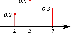
\includegraphics[width=0.4\textwidth]{images/spi/Discrete_probability_distrib}\hfill{}
\includegraphics[width=0.4\textwidth]{images/spi/Fair_dice_probability_distribution}\hfill{}

\caption{\textbf{(1)} Ukázka grafu pravděpodobnostní funkce. Všechny hodnoty
této funkce musí být nezáporné a jejich součet je $1$. \textbf{(2)}
Pravděpodobnostní funkce poctivé kostky. U všech čísel na kostce je
stejná pravděpodobnost.~{[}\faWikipediaW~\protect\href{https://en.wikipedia.org/wiki/Probability_mass_function}{EnWiki/Probability\_mass\_function}{]}}
\end{figure}

Pro spojitou náhodnou veličinu nemá smysl definovat pravděpodobnostní
funkci, protože u spojité veličiny je integrál v určitém bodě vždy
nulový. Místo ní definujeme hustotu pravděpodobnosti.

\subsection{Distribuční funkce ($F\left(x\right)$)}
\begin{center}
\begin{tabular}{|l|l|}
\hline 
\textbf{Další možná značení} & $F\left(x\right),\,F_{X}\left(x\right)$\tabularnewline
\hline 
\textbf{Určeno pro} & diskrétní i spojité náhodné veličiny\tabularnewline
\hline 
\end{tabular}
\par\end{center}

Pomocí pravděpodobnostní funkce lze zavést tzv. distribuční funkci
(CDF, Cumulative Distribution Function) vztahem:

\[
F\left(x\right)=P\left(X\leq x\right),\,x\in\mathbb{R}
\]

Distribuční funkce $F$ vyjadřuje pravděpodobnost, že náhodná veličina
(její volání, tj.~nějaké reálné číslo) má hodnotu menší nebo rovnou
reálnému číslu $x$. Distribuční funkce je neklesající a je spojitá
zprava.

Každá distribuční funkce má tyto vlastnosti:
\begin{enumerate}
\item Hodnoty distribuční funkce leží v rozsahu: 
\[
0\leq F\left(x\right)\leq1
\]
\item Pro \textbf{diskrétní} náhodnou veličinu $X$ lze pro libovolné reálné
číslo $x$ vyjádřit distribuční funkci vztahem:
\[
F\left(x\right)={\displaystyle \sum_{t<x}P\left(t\right)}
\]
\item Distribuční funkce je neklesající, tj. pro všechna $x_{2}>x_{1}$
platí:
\[
x_{2}>x_{1}:\,F\left(x_{2}\right)\geq F\left(x_{1}\right)
\]
\item ${\displaystyle \lim_{x\rightarrow-\infty}F\left(x\right)=0},\,{\displaystyle \lim_{x\rightarrow+\infty}F\left(x\right)=1}$
\end{enumerate}
\begin{figure}[H]
\centering

\includegraphics[width=1\textwidth]{\string"images/spi/spojita vs diskretni distribucni funkce\string".png}

\caption{Kumulativní distribuční funkce (CDF) pro diskrétní a spojitou náhodnou
veličinu.~{[}Lection02/Slide31{]}}
\end{figure}


\subsection{Hustota pravděpodobnosti, Probability Density Function ($f_{X}\left(x\right)$)}
\begin{center}
\begin{tabular}{|l|l|}
\hline 
\textbf{Další možná značení} & $f_{X}\left(x\right)$, $f\left(x\right)$, PDF\tabularnewline
\hline 
\textbf{Určeno pro} & pouze spojité náhodné veličiny\tabularnewline
\hline 
\end{tabular}
\par\end{center}

Rozdělení pravděpodobnosti spojité náhodné veličiny se určuje prostřednictvím
funkce, kterou označujeme jako hustota rozdělení pravděpodobnosti
(hustota pravděpodobnosti).
\begin{itemize}
\item Pravděpodobnost, že spojitá náhodná veličina nabývá určité přesně
dané hodnoty je nulová.
\item Obecně neplatí, že i hustota pravděpodobnosti spojité veličiny bude
spojitá.
\end{itemize}
Hustota pravděpodobnosti $f\left(x\right)$ spojité náhodné veličiny
$X$ je nezáporná reálná funkce taková, že pro všechna reálná $x$
se dá distribuční funkce $F\left(x\right)$ náhodné veličiny $X$
vyjádřit ve tvaru
\[
F\left(x\right)=\intop_{-\infty}^{x}f\left(t\right)\text{d}t
\]
Obsah plochy mezi touto křivkou $f\left(x\right)$ a osou $x$ v jakémkoliv
intervalu je pravděpodobnost, že $X$ nabude hodnoty z tohoto intervalu.
To ostatně plně odpovídá tomu, jak jsme hustotu definovali – připomeňme,
že integrál z křivky je vlastně velikost plochy pod touto křivkou.

Vlastností každé hustoty pravděpodobnosti je, že celá plocha pod křivkou
dává dohromady jedničku. To je analogické situaci u diskrétní náhodné
veličiny, kde součet pravděpodobností všech možných výsledků rovněž
dával jedničku. Pokud tuto vlastnost zapíšeme matematicky, dostáváme
rovnici: 
\[
\intop_{-\infty}^{+\infty}f\left(x\right)\text{d}x=1
\]

\begin{flushright}
\cite{Iastat-2001}
\par\end{flushright}

\begin{figure}[H]
\centering

\includegraphics[width=0.7\textwidth]{\string"images/spi/hustota pravdepodobnosti\string".png}

\caption{Hustota pravděpodobnosti spojité náhodné veličiny $X$.~{[}Lec02/Slide37{]} }
\end{figure}


\subsection{Střední hodnota $\mathbb{E}X$\label{subsec:St=000159edn=0000ED-hodnota}}

Střední hodnota je charakteristika náhodné veličiny. Jedná se o vážený
průměr\footnote{Vážený průměr zobecňuje aritmetický průměr a poskytuje charakteristiku
statistického souboru v případě, že hodnoty v tomto souboru mají různou
důležitost, různou váhu. } hodnot, které veličina $X$ nabývá. Většina výsledků náhodných pokusů
by se tedy měla pohybovat okolo této hodnoty.

\begin{minipage}[t]{1\columnwidth}%
Pro diskrétní náhodné veličiny vypočteme střední hodnotu jako:

\begin{eqnarray*}
\mathbb{E}X & = & \sum_{i}p_{i}x_{i}=\sum_{i}x_{i}*\mathbb{P}\left(X=x_{i}\right)
\end{eqnarray*}
%
\end{minipage}

\begin{minipage}[t]{1\columnwidth}%
Pro spojité náhodné veličiny vypočteme střední hodnotu jako:

\[
\mathbb{E}X=\intop_{-\infty}^{+\infty}x*f_{x}\left(x\right)\text{d}x
\]

\begin{center}
($P$ a $f$ jsou funkce hustoty.)
\par\end{center}%
\end{minipage}

Pro libovolné náhodné veličiny $\mathbb{E}\left(X\right)<\infty,\,\mathbb{E}\left(Y\right)<\infty$
a konstanty $a,\,b\in\mathbb{R}$ platí:

\begin{minipage}[t]{1\columnwidth}%
\begin{eqnarray*}
\mathbb{E}\left(aX+Y\right) & = & a\mathbb{E}\left(X\right)+\mathbb{E}\left(Y\right)~\text{(linearita)}\\
\mathbb{E}\left(X\pm Y\right) & = & \mathbb{E}\left(X\right)\pm\mathbb{E}\left(Y\right)\\
\mathbb{E}\left(X+Y\right) & = & \mathbb{E}\left(max\left\{ X,\,Y\right\} \right)+\mathbb{E}\left(min\left\{ X,\,Y\right\} \right)\\
\mathbb{E}X^{2} & = & \sum_{i}p_{i}x_{i}^{2}\,\text{(pro diskrétní jevy)}\\
\mathbb{E}\left(\text{max}\left\{ X,\,Y\right\} \right) & = & \mathbb{E}\left(X\right)+E\left(Y\right)-\mathbb{E}\left(\text{min}\left\{ X,\,Y\right\} \right)\\
\mathbb{E}\left(XY\right) & = & \mathbb{E}\left(X\right)*\mathbb{E}\left(Y\right)\,\text{(platí jen pro nezávislé jevy)}
\end{eqnarray*}
%
\end{minipage}

\subsection{Momenty náhodné proměnné~\texorpdfstring{\faGraduationCap}{(*)}}

Jedna z charakteristik pravděpodobnostního rozdělení. 
\begin{center}
{\fboxsep 10pt\shadowbox{\begin{minipage}[t]{0.9\columnwidth}%
\smallskip{}

\textbf{\uline{Notace}}

\smallskip{}

\begin{align*}
EX^{k} & ==E\left(X^{k}\right)\\
E\left(X-\mu_{1}\right)^{k} & ==E\left(\left(X-\mu_{1}\right)^{k}\right)\\
\mu & ==\mu_{X}==\mu_{1}==EX\\
\text{var\ensuremath{\left(X\right)}} & ==\sigma_{X}^{2}==\sigma^{2}==E\left(X-\mu\right)^{2}\\
\sigma_{X} & ==\sigma==\sqrt{\text{var}\left(X\right)}
\end{align*}

\begin{flushright}
{[}Lecture02/Slide43{]}
\par\end{flushright}
\smallskip{}
%
\end{minipage}}}
\par\end{center}

\subsubsection{Obecný (necentrální) moment}

Momenty rozdělení jsou střední hodnoty mocnin příslušné náhodné veličiny. 

$K$-tý \textbf{obecný} (\textbf{necentrální}) \textbf{moment} náhodné
veličiny $X$ je definován vzorcem
\[
\mu_{k}^{'}=m_{k}=\mathbb{E}\left[X^{k}\right]\text{.}
\]
Pro diskrétní náhodné veličiny lze tedy psát
\[
\mu_{k}^{'}={\displaystyle \sum_{i=1}^{\infty}x_{i}^{k}}p_{i}
\]
a pro spojité náhodné veličiny
\[
\mu_{k}^{'}={\displaystyle \intop_{-\infty}^{\infty}x^{k}f\left(x\right)}\text{d}x
\]
kde $f\left(x\right)$ je hustota rozdělení dané veličiny.

Poslední dva tvary vycházejí z výpočtu střední hodnoty viz \nameref{subsec:St=000159edn=0000ED-hodnota}~na~straně~\pageref{subsec:St=000159edn=0000ED-hodnota}.
První obecný moment se nazývá střední hodnota ($\mathbb{E}\left[X^{\highlight{1}}\right]$)
a a označuje se symbolem $\mu$.
\begin{flushright}
{[}\href{https://cs.wikipedia.org/wiki/Obecn\%C3\%BD_moment}{CsW/Obecný\_moment}{]}
\par\end{flushright}

\paragraph{Výběrový obecný moment}

$K$-tý \textbf{výběrový} obecný moment je definován vzorcem

\[
m_{k}^{'}=M_{k}^{'}=\frac{1}{n}{\displaystyle \sum_{i=1}^{n}x_{i}^{k}}
\]

První výběrový obecný (necentrální) moment aka \textbf{výběrový průměr}
je definován:
\[
\overline{X}_{n}=\frac{1}{n}{\displaystyle \sum_{i=1}^{n}X_{i}}
\]
s označuje se $\overline{X}_{n}$ (do předchozího vzorce jsme pouze
dosadili $k=1$).

\subsubsection{Centrální moment}

Místo obecných momentů vyšších řádů se častěji používají centrální
momenty. $K$-tý\textbf{ centrální moment} náhodné veličiny $X$ je
definován vzorcem
\[
\sigma_{k}=\mathbb{E}\left[\left(X-\mu_{1}\right)^{k}\right]\text{.}
\]

\begin{flushright}
{[}\href{https://cs.wikipedia.org/wiki/Obecn\%C3\%BD_moment}{CsWiki/Obecný\_moment},
Lecture02/Slide43{]}
\par\end{flushright}

\paragraph{Výběrový centrální moment}

Výběrový centrální moment je definován vzorcem

\[
m_{k}=M_{k}=\frac{1}{n}{\displaystyle \sum_{i=1}^{n}\left(X_{i}-\overline{X}\right)^{k}}
\]
kde $\overline{X}$ je výběrový průměr.
\begin{flushright}
{[}\href{https://cs.wikipedia.org/wiki/Centr\%C3\%A1ln\%C3\%AD_moment}{CsWiki/Centrální\_moment}{]}
\par\end{flushright}

\subsection{Rozptyl ($\sigma^{2},\,\text{var}\left(X\right),\,D\left(X\right)$)}

Druhý centrální moment náhodné veličiny – variabilita souboru náhodných
hodnot kolem její střední hodnoty.

Rozptyl je charakteristika náhodné veličiny. Rozptyl je definován
jako střední hodnota kvadrátů odchylek od střední hodnoty. Odchylku
od střední hodnoty, která má rozměr stejný jako náhodná veličina,
zachycuje směrodatná~odchylka~$\sigma$ .

Pro diskrétní náhodnou veličinu jej můžeme definovat takto: od každé
naměřené hodnoty odečteme průměr všech naměřených hodnot.:
\[
\sigma^{2}=\sum_{i=1}^{n}\left[x_{i}-E\left(X\right)\right]^{2}p_{i}=\sum_{i=1}^{n}x_{i}^{2}p_{i}-\left[E\left(X\right)\right]^{2}
\]

Pro spojitou náhodnou veličinu definujeme rozptyl vztahem:

\[
\sigma^{2}=\intop_{-\infty}^{+\infty}\left[x_{i}-E\left(X\right)\right]^{2}f\left(x\right)\text{d}x=\intop_{-\infty}^{+\infty}x_{i}^{2}f\left(x\right)\text{d}x-\left[E\left(X\right)\right]^{2}
\]

Dále platí pro libovolné náhodné veličiny $X$ a $Y$, $\text{var}\left(X\right)<\infty,\,\text{var}\left(Y\right)<\infty$
a konstanty $a,\,b\in\mathbb{R}$:

\begin{eqnarray*}
\text{var}\left(X\right) & = & E\left\{ \left[X-E\left(X\right)\right]^{2}\right\} =E\left(X^{2}\right)-\left[E\left(X\right)\right]^{2}\\
\text{var}\left(0\right) & \geq & 0\\
\text{var}\left(a\right) & = & 0\\
\text{var}\left(X\right) & = & \text{cov}\left(X,\,X\right)\\
\text{var}\left(a*X\right) & = & a^{2}*\text{var}\left(X\right)\\
\text{var}\left(X+a\right) & = & \text{var}\left(X\right)\\
\text{var}\left(X\pm Y\right) & = & \text{var}\left(X\right)+\text{var}\left(Y\right)\pm2*\text{cov}\left(X,\,Y\right)
\end{eqnarray*}

$E\left(X^{2}\right)-\left[E\left(X\right)\right]^{2}$ resp. zjednodušeně
$E\left(X^{2}\right)-E^{2}\left(X\right)$ je tzv. výpočetní tvar
rozptylu kde$E^{2}\left(X\right)$ je pouze druhá mocnina této hodnoty
a pro diskrétní náhodnou veličinu platí
\[
E\left(X^{2}\right)={\displaystyle \sum_{i}x_{i}^{2}*p_{i}}\text{.}
\]
Ekvivalentně pro spojitou náhodnou veličinu platí
\[
E\left(X^{2}\right)=\intop_{-\infty}^{+\infty}x^{2}*f\left(x\right)\text{d}x\text{.}
\]
Kde $p$ a $f$ jsou pravděpodobnostní funkce resp. funkce hustoty.

\subsection{Směrodatná odchylka ($\sigma$)}

Odmocnina z rozptylu náhodné veličiny $X$.
\[
\sigma=\sqrt{\text{var}\left(X\right)}
\]
Směrodatná odchylka je hodnota, o kterou se v obou směrech neodchyluje
od průměru více než $50\,\%$~hodnot.

\section{Rozdělení pravděpodobnosti}

Rozdělení pravděpodobnosti náhodné veličiny je všeobecný vzorec, který
popisuje chování náhodné veličiny za různých podmínek\footnote{Chování náhodné veličiny za různých podmínek říká, jaké hodnoty nabude
náhodná veličina (počet padnutí šestky na hrací kostce) při měnících
se podmínkách (počet stran kostky, počet hodů, atp.).}.

Rozdělení pravděpodobnosti nebo rozložení pravděpodobnosti (někdy
také distribuce pravděpodobnosti) náhodné veličiny je pravidlo, kterým
\textbf{každému jevu popisovanému touto veličinou přiřazujeme určitou
pravděpodobnost}. Rozdělení pravděpodobnosti náhodné veličiny tedy
získáme, pokud každé hodnotě diskrétní náhodné veličiny, popř. intervalu
hodnot spojité náhodné veličiny, přiřadíme pravděpodobnost.
\begin{flushright}
{[}\faWikipediaW~\href{https://cs.wikipedia.org/wiki/Rozd\%C4\%9Blen\%C3\%AD_pravd\%C4\%9Bpodobnosti}{CsWiki/Rozdělení\_pravděpodobnosti}{]}
\par\end{flushright}

Rozdělení (distribuce) pravděpodobnosti lze také chápat jako zobrazení,
které každému elementárnímu jevu přiřazuje určité reálné číslo, které
charakterizuje pravděpodobnost tohoto jevu.

\begin{table}[H]
\centering

\begin{tabular}{|l|c|}
\hline 
\textbf{\cellcolor{lightgray}Distribuční funkce} ($F$) & $X\leq k$\tabularnewline
\hline 
\textbf{\cellcolor{lightgray}Hustota/Pravděpodobnost} & $X=k$\tabularnewline
\hline 
\textbf{\cellcolor{lightgray}Funkce přežití} & $X>k$\tabularnewline
\hline 
\end{tabular}

\caption{Funkce a nerovnosti}
\end{table}


\subsection{Binomické rozdělení /diskrétní/}
\begin{itemize}
\item \textbf{A:} Binomické rozdělení říká pravděpodobnost, že se v sérii
pokusů ($n$) bude vyskytovat jev, který má nějakou pravděpodobnost
($p$) právě $X$-krát.
\item \textbf{B: }Náhodná veličina $X\sim\text{Binom}\left(n,\,p\right)$
udává celkový počet úspěchů v posloupnosti $n$ nezávisle opakovaných
pokusů, přičemž v každém z těchto pokusů nastává „úspěch“ s pravděpodobností
$p$, kde $p\in\left(0,1\right)$ a $n$ je přirozené číslo.
\end{itemize}
\begin{align*}
X & \sim\text{Binom}\left(n,\,p\right)
\end{align*}

Speciální příklad binomického rozdělení je \textbf{Bernoulliho rozdělení},
kde
\[
n=1
\]
a tedy
\[
X\sim\text{Binom}\left(1,\,p\right)
\]

\begin{table}[H]
\centering

\begin{tabular}{|c|c|c|c|c|}
\hline 
\rowcolor{lightgray}\textbf{Značení} & \textbf{Pravděpodobnostní f.} & \textbf{Distribuční f.} & $\mathbb{E}X$ & $\text{var}X$\tabularnewline
\hline 
\hline 
$X\sim\text{Binom}\left(n,\,p\right)$ & $P\left(X=x\right)=\binom{n}{x}p^{x}q^{n-x}$ & $P\left(X\leq k\right)={\displaystyle \sum_{i\leq k}p^{i}\left(1-p\right)^{n-i}}$ & $n*p$ & $n*p*q$\tabularnewline
\hline 
\end{tabular}

\caption{Parametry binomického rozdělení}
\end{table}
\begin{minipage}[t]{1\columnwidth}%
Kde 
\begin{itemize}
\item $n$ je počet nezávislých náhodných pokusů (např. počet hodů kostkou);
\item $p$ říká, jaká je pravděpodobnost jevu, který sledujeme (např. pravděpodobnost,
že na kostce padne šestka);
\item $q$ je pravděpodobnost, že daný jev nenastane, $q$ vypočítáme jako
\[
q=1-p
\]
\end{itemize}
%
\end{minipage}

Kombinační číslo\footnote{Na kalkulačce se jedná o funkci \colorbox{lightgray}{\texttt{nCr}}.}
spočteme
\[
\binom{n}{k}=\frac{n!}{k!\left(n-k\right)!}
\]


\subsection{Geometrické /diskrétní/}

\begin{table}[H]
\centering

\begin{tabular}{|c|c|c|c|c|}
\hline 
\rowcolor{lightgray}\textbf{Značení} & \textbf{Pravděpodobnostní f.} & \textbf{Distribuční f.} & $\mathbb{E}X$ & $\text{var}X$\tabularnewline
\hline 
\hline 
$X\sim\text{Geom}\left(p\right)$ & $P\left(X=x\right)=\left(1-p\right)^{k-1}*p$ & $P\left(X\leq k\right)={\displaystyle 1-\left(1-p\right)^{n}}$ & $\frac{1}{p}$ & $\frac{1-p}{p^{2}}$\tabularnewline
\hline 
\end{tabular}

\caption{Parametry geometrického rozdělení}
\end{table}


\subsection{Poissonovo rozdělení /diskrétní/\label{subsec:Poissonovo-rozd=00011Blen=0000ED-/diskr=0000E9tn=0000ED/}}

Poissonovo rozdělení\footnote{Eulerovo číslo $\mathrm{e}\thickapprox2,718$. }
má dvě hlavní oblasti použití:
\begin{enumerate}
\item Stejná oblast použití jako rozdělení binomické. Pomocí Poissonova
rozdělení je možné aproximovat binomické rozdělení, zapisujeme $\mathrm{Binom}\left(n,p\right)\approx\text{Pois}\left(\lambda=np\right)$
za podmínek, že počet pokusů $n\rightarrow\infty$, pravděpodobnost
výskytu $p\rightarrow0$ a $np$ je konečné číslo. V tomto případě
je parametr $\lambda=np$ (to je střední hodnota binomického rozdělení).
Tato aproximace se považuje za výhodnou pro~$n\geq30$ (počet pokusů)~a~$p\leq0,1$
(tedy pravděpodobnost každého z pokusů je malá, tj.~$<10\%$).~\cite{Budikova-2016}
\[
X\sim\text{Pois}\left(\lambda\right),\,\lambda=p*n
\]
\item Druhou důležitou oblastí použití Poissonova rozdělení jsou Poissonovské
proudy. Zpravidla jde o příklady, ve~kterých řešíme pravděpodobnost
výskytu nějakého jevu (např. počet výběrů z~bankomatu) za určitou
časovou jednotku (např. 10 minut). Parametr $\lambda>0$ udává \textbf{průměrný
počet výskytu jevu za určitou časovou jednotku} – \textbf{\textcolor{purple}{\uline{intenzita}}}.
Ve vzorci pravděpodobnostní funkce se navíc nachází parametr $t$,
který udává velikost sledovaného časového intervalu~\cite{Pcola}
\begin{align*}
N\left(t\right)\sim\text{Poisson}\left(\lambda t\right)\\
\left[P\left(N\left(t\right)=n\right)\right]=P\left(X=x\right)=\frac{\left(t\lambda\right)^{x}}{x!}\mathrm{e}^{-t\lambda}
\end{align*}
Vzorec říká pravděpodobnost, že během časového intervalu $\left(0,\,t\right)$
nastane přesně~$x$~událostí (resp. $n$), kde $t$ je čas.
\end{enumerate}
\begin{table}[H]
\centering

\begin{tabular}{|c|c|c|c|c|}
\hline 
\rowcolor{lightgray}\textbf{Značení} & \textbf{Pravděpodobnostní f.} & \textbf{Distribuční f.} & $\mathbb{E}X$ & $\text{var}X$\tabularnewline
\hline 
\hline 
$X\sim\text{Pois}\left(\lambda\right)$ & $P\left(X=x\right)=\frac{\lambda^{x}}{x!}\mathrm{e}^{-\lambda}$ & $Q\left(\left\lfloor k+1\right\rfloor ,\,\lambda\right)$ & $\lambda$ & $\lambda$\tabularnewline
\hline 
\end{tabular}

\caption{Parametry Poissonova rozdělení. Pravděpodobnostní funkce nemá parametr
$t$, protože v tomto kontextu říká, \glqq pravděpodobnost, že během
\textbf{intervalu jednotkové délky} dojde k přesně $x$ událostem``.}
\end{table}


\subsection{Studentovo $t$-rozdělení /spojité/}

Studentovo $t$-rozdělení je spojité rozdělení pravděpodobnosti, které
umožňuje i na základě souborů dat s malými rozsahy, u kterých nelze
mluvit o~asymptoticky normálním rozdělení, dělat přijatelné závěry 

Pro hodnoty $n>30$ je rozdělení $t$ velmi blízké normovanému normálnímu
rozdělení.

\subsection{Exponenciální rozdělení /spojité/\label{subsec:Exponenci=0000E1ln=0000ED-rozd=00011Blen=0000ED-/spojit=0000E9}}

\begin{tabular}{|c|c|}
\hline 
\cellcolor{lightgray}\textbf{Paměť?} & \textbf{Bez paměti}\tabularnewline
\hline 
\end{tabular}

Toto rozdělení má spojitá náhodná veličina $X$, která představuje
\textbf{dobu čekání do~nastoupení} (Poissonovského) náhodného jevu,
nebo délku intervalu (časového nebo délkového) mezi takovými dvěma
jevy (např. doba čekání na obsluhu, vzdálenost mezi dvěma poškozenými
místy na silnici). 

Příklady aplikace:
\begin{itemize}
\item doba životnosti výrobku (tedy čekání na jeho poruchu);
\item doba čekání ve frontě;
\item doba mezi dvěma poruchami;
\item modelování času radioaktivního rozpadu částic.
\end{itemize}
Jestliže Poissonovo rozdělení modelovalo počet nějakých událostí v
čase, exponenciální rozdělení se používá k modelování doby výskytu
příslušné události. Ve vzorcích se~vyskytuje~intenzita $\lambda$. 
\begin{flushright}
\cite{Homen-2013}
\par\end{flushright}

Exponenciální rozdělení je \textbf{bez paměti}. Předpokládejme dobu
čekání $T\sim\text{Exp}\left(\lambda\right)$. Pakliže jsme již čekali
$s$ jednotek času, zbývající čekací čas $T-s$ má stejné rozdělení
– tedy situace je stejná, jako kdybychom ještě vůbec nečekali

\footnote{Čekáme na metro, u kterého nevíme, kdy přijede. Pravděpodobnost, že
\glqq teď už přijede`` je stále stejná nehledě na to, zda už čekáme
$5$ minut.}. Formálně zapsáno platí
\[
T\sim\text{Exp}\left(\lambda\right)\,\Rightarrow\,\left(T-s|T>s\right)\sim\text{Exp}\left(\lambda\right)
\]
kde
\begin{itemize}
\item $T>s$ je čas, který jsme již čekali, ale nenastal žádný příchod události;
\item $T-s$ je zbývající čas k čekání.
\end{itemize}
\begin{flushright}
{[}Lecture12/Slide07{]}
\par\end{flushright}

\begin{table}[H]
\centering

\begin{tabular}{|c|c|c|c|c|}
\hline 
\rowcolor{lightgray}\textbf{Značení} & \textbf{Hustota} & \textbf{Distribuční f.} & $\mathbb{E}X$ & $\text{var}X$\tabularnewline
\hline 
\hline 
$X\sim\text{Exp}\left(\lambda\right)$ & $\begin{cases}
\lambda\mathrm{e}^{-\lambda x} & ;\,x>0\\
0 & ;\,x\leq0
\end{cases}$ & $\begin{cases}
1-\lambda\mathrm{e}^{-\lambda x} & ;\,x>0\\
0 & ;\,x\leq0
\end{cases}$ & $\frac{1}{\lambda}$ & $\frac{1}{\lambda^{2}}$\tabularnewline
\hline 
\end{tabular}

\caption{Parametry exponenciálního rozdělení}
\end{table}

\begin{figure}[H]
\centering


\includegraphics[width=0.85\textwidth]{images/spi/Exponential_pdf}

\caption{Graf hustoty exponenciálního rozdělení s různými hodnotami parametru
$\lambda$.}
\end{figure}

\begin{flushright}
{[}\href{https://cs.wikipedia.org/wiki/Exponenci\%C3\%A1ln\%C3\%AD_rozd\%C4\%9Blen\%C3\%AD}{CsWiki/Exponenciální rozdělění}{]}
\par\end{flushright}

\subsection{Normální (Gaussovo) /spojité/\label{subsec:Norm=0000E1ln=0000ED-(Gaussovo)-/spojit=0000E9/}}

Nejdůležitějším rozdělením v teorii pravděpodobnosti je normální rozdělení,
také nazývané Gaussovo. Jeho význam spočívá v tom, že za určitých
podmínek dobře aproximuje mnoho jiných (nejen spojitých, ale i diskrétních)
pravděpodobnostních rozdělení.. Značíme jej
\[
X\sim\text{N}\left(\mu,\,\sigma^{2}\right)
\]

\begin{itemize}
\item kde směrodatná odchylka $\sigma>0$;
\item $\mu$ je vážený průměr (střední hodnota), určuje, kde má Gaussova-Laplaceova
křivka maximum;
\item $\sigma^{2}$ je rozptyl.
\end{itemize}
\begin{flushright}
\cite{Budikova-2016}
\par\end{flushright}

\begin{figure}[H]
\centering

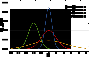
\includegraphics[width=0.85\textwidth]{images/spi/Normal_Distribution_PDF}

\caption{Gaussova-Laplaceova křivka. Grafy hustot (Probability density function)
normálního rozdělení s různými charakteristikami. Parametr $\mu$
určuje, kde má křivka maximum. Parametr $\sigma$ (směrodatná odchylka)
určuje, jak jsou po obou stranách od hodnoty $\mu$ vzdáleny inflexní
body {\footnotesize{}(křivka se mění z konkávní na konvexní nebo obráceně)}
($\mu-\sigma,\,\mu+\sigma$), tedy jak jak je křivka roztažena do~šířky.~\cite{Homen-2013}}
\end{figure}

\begin{figure}[H]
\centering

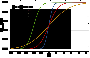
\includegraphics[width=0.85\textwidth]{images/spi/Normal_Distribution_CDF}

\caption{Grafy distribučních funkcí (Cumulative distribution function) normálního
rozdělení s různými charakteristikami.}
\end{figure}

\begin{table}[H]
\centering

\begin{tabular}{|c|c|c|c|c|}
\hline 
\rowcolor{lightgray}\textbf{Značení} & \textbf{Hustota} & \textbf{Distribuční f.} & $\mathbb{E}X$ & $\text{var}X$\tabularnewline
\hline 
\hline 
$X\sim\text{N}\left(\mu,\,\sigma^{2}\right)$ & $f_{X}\left(x\right)=\frac{1}{\sigma\sqrt{2\pi}}*e^{\nicefrac{-\left(x-\mu\right)^{2}}{2\sigma^{2}}}$ & složitá & $\mu$ & $\sigma^{2}$\tabularnewline
\hline 
\end{tabular}

\caption{Parametry normálního rozdělení}
\end{table}

Normální rozdělení s parametry $\mu=0$ a $\sigma^{2}=1$ nazýváme
\textbf{standardizované (normované) normální rozdělení}, které má
tvar:
\[
U=\frac{x-\mu}{\sigma}\sim N\left(\mu=0,\,\sigma^{2}=1\right),\,X\left(\omega\right)=x,\,x\in\mathbb{R}
\]
a značíme jej $U\sim\text{N}\left(0,\,1\right)$, kde $U$ (někdy
značeno jako $Z$) je \textbf{normovaná veličina}. Distribuční funkci
značíme jako $\Phi\left(u\right)$, její hodnoty jsou tabelované. 

Celý zápis je tedy
\[
P\left(X\leq x\right)=\Phi\left(\frac{x-\mu}{\sigma}\right)=\alpha
\]

\begin{figure}[H]
\centering

\includegraphics[width=0.5\textwidth]{\string"images/spi/hustota normovaneho normalniho rozdeleni\string".png}

\caption{Graf hustoty normovaného normálního rozdělení.~{[}Lecture04/Slide34{]}}
\end{figure}

\begin{center}
{\fboxsep 10pt\shadowbox{\begin{minipage}[t]{0.9\columnwidth}%
\smallskip{}

\textbf{\uline{Tabulky}}

\smallskip{}

Pro zjištění hodnot distribuční funkce musíme mít po ruce \glqq Standard
normal distribution table``. V těchto tabulkách se někdy $U$ značí
jako $Z$. Struktura tabulek je následující.
\[
\begin{array}{ccccc}
Z/U & .\text{␣} & .\text{␣␣} & .\text{␣␣␣} & .\text{␣␣␣␣}\\
\Phi\left(U\right) & \ldots & \ldots & \ldots & \ldots\\
\Phi\left(U\right) & \ldots & \alpha & \ldots & \ldots\\
\Phi\left(U\right) & \ldots & \alpha & \ldots & \ldots\\
\Phi\left(U\right) & \ldots & \ldots & \ldots & \ldots
\end{array}
\]

Při zjišťování hodnoty je třeba si uvědomit, zda hledáme 
\begin{enumerate}
\item ${P\left(U\leq\boldsymbol{\alpha}\right)=0,95}$ (víme pravděpodobnost,
nevíme bod /kvantil/ na ose $x$) nebo
\item $P\left(U\leq1,645\right)=\boldsymbol{x}$ (známe bod /kvantil/ na
ose $x$ a pro něj hledáme hodnotu distribuční funkce).
\end{enumerate}
Tabulky hodnot jsou omezeny pouze na $u\geq0$ (nezáporné normované~$u$),
pro $u<0$ (záporné~$u$) platí vztah:
\[
\Phi\left(-u\right)=1-\Phi\left(u\right)\text{.}
\]
Stejnou metodu použijeme pro zjištění distribuční funkce \glqq větší
než`` tj. 
\[
P\left(X>x\right)=1-P\left(X\leq x\right)
\]

\smallskip{}
%
\end{minipage}}}
\par\end{center}

\pagebreak{}

\part{Odhady parametrů statistických rozdělení a modelů, odhady hustoty
a~distribuční funkce~(I.~okruh) }

\begin{tcolorbox}[title=\faWarning~Hlášení chyb v prvním okruhu, colback=yellow!10, colframe=black!75!black, colbacktitle=yellow, coltitle=black, fonttitle=\bfseries]
\begin{flushleft}
Chyby a nedostatky v této sekci, prosím, hlaste na~\href{https://fit-wiki.cz/\%C5\%A1kola/p\%C5\%99edm\%C4\%9Bty/mi-spi/spi_szz/2017/spi_szz_okruh_1}{https://fit-wiki.cz/škola/předměty/mi-spi/spi\_szz/2017/spi\_szz\_okruh\_1}.
\par\end{flushleft}

\end{tcolorbox}

\section{Motivace}

{

\exhyphenpenalty=10\hyphenpenalty=10

\marginpar{\protect\begin{flushleft}
\textit{\textcolor{purple}{Z~výběru odhadujeme statistiky populace.}}\protect
\par\end{flushleft}}

}
\begin{itemize}
\item \textbf{Základní soubor} (\textbf{populace}) má svoje statistiky jako
jsou rozptyl a průměrná hodnota.
\item Tyto statistiky má i \textbf{výběrový soubor} (vybraný vzorek ze základního
souboru).
\end{itemize}
V praxi obvykle provádíme výběrové statistické šetření s cílem zkoumat
vlastnosti základního souboru (populace). Na základě výběrových dat
provádíme zevšeobecňující úsudek, tzn. usuzujeme na obecnější skutečnosti,
které se týkají celé populace. Jednou ze základních úloh statistického
usuzování (statistické indukce) je odhadování neznámých parametrů
základního souboru pomocí údajů získaných náhodným výběrem z daného
základního souboru. Důležitým rysem statistické metody odhadování
je její pravděpodobnostní charakter (při jakémkoli úsudku, který o
základním souboru učiníme na základě údajů získaných náhodným výběrem,
musíme počítat s možností, že tento úsudek je chybný). 

\textbf{Podle typu rozdělení, kterým se řídí základní soubor je možno
na základě dat výběrových souborů z tohoto rozdělení zjistit různé
charakteristiky, které se v jistém smyslu blíží k~odpovídajícím charakteristikám
základního souboru (jsou jejich odhadem).} Odhadování parametrů základního
souboru na základě charakteristik výběrových souborů lze provést v
zásadě \textbf{dvěma metodami}:
\begin{enumerate}
\item \textbf{\textcolor{purple}{\uline{Bodový odhad}}} – neznámý parametr
základního souboru odhadujeme pomocí \textbf{jediného čísla}, bodu.
Bodovým odhadem parametru základního souboru jsou popisné charakteristiky
výběrového souboru. 
\item \textbf{\textcolor{purple}{\uline{Intervalový odhad}}} – neznámý
parametr základního souboru odhadujeme pomocí dolní a horní hranice
intervalu hodnot, mezi nimiž se parametr základního souboru nachází
s určitou pravděpodobností. 
\end{enumerate}
Intervalové odhady parametrů základního souboru umožňují vyjádřit
chybu, kterou je odhad parametru základního souboru na základě statistik
výběrového souboru zatížen. Naproti tomu bodový odhad parametru základního
souboru pomocí charakteristiky výběrového souboru je zatížen určitou
chybou odhadu, nepřesností. Tato chyba je tím menší, čím větší je
rozsah $n$ výběrového souboru.

\section{Základní pojmy}

(Následující pojmy jsou rovněž definovány i v úvodu tohoto dokumentu,
připomeňme je však i zde těmito zjednodušenými definicemi.)
\begin{description}
\item [{Náhodný~výběr}] Náhodný výběr $X=\left(X_{1},\,X_{2},\,X_{3},\,\ldots X_{n}\right)$
je vektor náhodných veličin, které jsou nezávislé a mají stejné rozdělení.
Provedením pokusu dostaneme realizaci náhodného výběru ${x=\left(x_{1},\,x_{2},\,\ldots,\,x_{n}\right)\in\mathbb{R}^{n}}$,
kde $n$ je rozsah výběru.
\item [{Střední~hodnota}] Je vážený průměr daného rozdělení.
\item [{Rozptyl}] Druhý centrální moment náhodné veličiny. Jedná se o charakteristiku
variability rozdělení pravděpodobnosti náhodné veličiny, která vyjadřuje
variabilitu souboru náhodných hodnot kolem její střední hodnoty.
\item [{Směrodatná~odchylka}] Kvadratický průměr odchylek hodnot znaku
od jejich aritmetického průměru\footnote{Jednoduše se jedná o druhou odmocninu aritmetického průměru.}.
\end{description}
\begin{flushright}
\cite{Navara-2010}
\par\end{flushright}

\section{Centrální limitní věta, The Central Limit Theorem (CLT)~\texorpdfstring{\faGraduationCap}{(*)}}

{

\exhyphenpenalty=10\hyphenpenalty=10

\marginpar{\protect\begin{flushleft}
\textit{\textcolor{purple}{Výběrový průměr se blíží normálnímu rozdělení.}}\protect
\par\end{flushleft}}

}

Tvrzení, podle něhož se rozdělení výběrového průměru po vhodné normalizaci
blíží k~normálnímu rozdělení.

Podstatou centrální limitní věty je tvrzení, že náhodná veličina~$X$,
která vznikla jako součet velkého počtu \textbf{vzájemně nezávislých
stejně rozdělených náhodných veličin} $X_{1},\,X_{2},\,\ldots,\,X_{n}$,
má za velmi obecných podmínek přibližně normální rozdělení. Říkáme,
že náhodná veličina $X$, jejíž limitním zákonem rozdělení je rozdělení
normální, má~tzv.~\textbf{asymptoticky normální rozdělení}. 
\begin{flushright}
\cite{Budikova-2016}
\par\end{flushright}

Pro stejně rozdělené náhodné veličiny platí \textbf{Lindebergova-Lévyova
centrální limitní věta}: Jsou-li $X_{1},\,X_{2},\,\ldots,\,X_{n}$
\textbf{nezávislé stejně rozdělené} náhodné veličiny s konečným rozptylem,
pak pro každé $x\in\mathbb{R}$ 
\[
{\displaystyle \lim_{n\rightarrow\infty}}P\left[\frac{\left({\displaystyle \sum_{i=1}^{n}}X_{i}\right)-n\mathbb{E}X_{1}}{\sqrt{n\text{var}X_{1}}}<x\right]=\Phi\left(x\right)
\]

kde $\Phi$ je distribuční funkce standardního normálního rozdělení
$N\left(0,1\right)$.

To znamená, že je-li $S_{n}={\displaystyle \sum_{i=1}^{n}X_{i}}$
součtem velkého množství nezávislých náhodných veličin, můžeme její
rozdělení považovat za přibližně normální.
\[
S_{n}\overset{\centerdot}{\sim}N\left(n\mu,n\sigma^{2}\right)
\]

kde $\mu=\mathbb{E}X$ a $\sigma^{2}=\text{var}X_{1}$.

\section{Konfidenční intervaly (metoda intervalového odhadu)~\texorpdfstring{\faGraduationCap}{(*)}}

{

\exhyphenpenalty=10\hyphenpenalty=10

\marginpar{\protect\begin{flushleft}
\textit{\textcolor{purple}{Interval s~danou přesností. Interval spolehlivosti
= intervalový odhad nějakého parametru s~danou pravděpodobností =
konfidenční interval pro daný parametr}}\protect
\par\end{flushleft}}

}

Pokud zjišťujeme rozptyl nebo střední hodnotu základního souboru na
základě nějakého výběru z něj, konečný \textbf{výsledek udáváme} \textbf{v
intervalu}, protože není možné určit přesnou hodnotu. Pokud bychom
chtěli určit tento interval se stoprocentní pravděpodobností, byl
by takový interval v praxi příliš široký. Z~tohoto důvodu se tyto
intervaly uvádí na přesnostech nižších než $100\,\%$, a to obvykle
např. s~$95\,\%$ přesností, která nám poskytuje užší interval při
málo změněné věrohodnosti. Přesnost, se kterou udáváme výsledek, nazýváme
\textbf{konfidenční interval} (interval spolehlivosti), který značíme
jako
\[
1-\alpha
\]

kde $\alpha$ značí možnou chybu\footnote{Např. chceme-li interval s přesností $95\,\%$, zapíšeme výraz jako
$1-\alpha=0,95\rightarrow\alpha=0,05$.} (nebo-li hladinu významnosti). Následující tvar říká, že s~pravděpodobností
rovnou $1-\alpha$ se bude zjišťovaná hodnota $x$ základního souboru
nacházet v intervalu $\left(X,\,Y\right)$. Zjišťovanou hodnotou je
průměr nebo rozptyl.
\[
P\left(X<x<Y\right)=1-\alpha
\]

Existují oboustranné a jednostranné intervalové odhady, jednostranné
se dále dělí na levostranné a pravostranné.

\textbf{Kritické hodnoty rozdělení }na hladině významnosti $p$ jsou
kvantily, kde index $p$ vyjadřuje pravděpodobnost, že náhodná veličina
(u symetrických rozdělení její absolutní hodnota), překročí tuto hodnotu.
\begin{flushright}
\cite{Homen-2013}
\par\end{flushright}

\textbf{Kvantil} můžeme definovat jako libovolnou hodnotu náhodné
proměnné $X$, která rozděluje soubor dat na dvě části. 

\subsection{Zjišťování střední hodnoty $\mu$, intervalový odhad\label{subsec:Zji=000161=000165ov=0000E1n=0000ED-st=000159edn=0000ED-hodnoty}}
\begin{center}
{\fboxsep 10pt\fbox{\begin{minipage}[c]{0.7\columnwidth}%
\begin{flushleft}
Je důležité určit, zda známe nebo neznáme rozptyl. Pokud rozptyl známe,
použijeme normalizaci a normální rozdělení. Ve druhém případě použijeme
Studentovo rozdělení.
\par\end{flushleft}%
\end{minipage}}}
\par\end{center}

{

\exhyphenpenalty=10\hyphenpenalty=10

\marginpar{\protect\begin{flushleft}
\textit{\textcolor{purple}{Chceme $\mu$, }}\textbf{\textit{\textcolor{purple}{známe}}}\textit{\textcolor{purple}{{}
či }}\textbf{\textit{\textcolor{purple}{neznáme}}}\textit{\textcolor{purple}{{}
rozptyl?}}\protect
\par\end{flushleft}}

}

Chceme-li zjistit střední hodnotu základního souboru, mohou nastat
dvě situace:
\begin{enumerate}
\item \textbf{Známe rozptyl} $\sigma^{2}$ základního souboru.
\item \textbf{Rozptyl základního souboru neznáme}, a proto musíme použít
rozptyl z~výběrového souboru (tj.~\textbf{výběrový~rozptyl}~$s_{n}^{2}$).
Tento rozptyl je buď zadaný nebo jej spočteme. Příklady na výpočet
parametrů základního souboru bez toho, abychom znali jeho rozptyl,
jsou reálnější, jelikož v realitě opravdu většinou rozptyl základního
souboru není známý.
\end{enumerate}
\begin{center}
{\fboxsep 10pt\shadowbox{\begin{minipage}[t]{0.9\columnwidth}%
\textbf{\uline{Bodový odhad \mbox{$\mu$}}}

\smallskip{}

Nechť $X_{1},\,X_{2},\,X_{3},\,\ldots X_{n}$ jsou i.i.d.\footnote{idenpendent and identically distributed}
náhodné veličiny s konečným průměrem $\mu$ a rozptylem~$\sigma^{2}$.

Pro \textbf{odhad průměru $\mu$} použijeme průměr vzorku (tzv. první
výběrový obecný moment aka výběrový průměr)
\[
\overline{X}_{n}=\frac{1}{n}{\displaystyle \sum_{i=1}^{n}X_{i}}
\]

\begin{flushright}
{[}Lecture17/Slide7,~\href{https://cs.wikipedia.org/wiki/Obecn\%C3\%BD_moment}{CsWiki/Obecný\_moment}{]}
\par\end{flushright}
\smallskip{}
%
\end{minipage}}}
\par\end{center}

\subsection{Zjišťování střední hodnoty $\mu$, \textit{známe} rozptyl $\sigma^{2}$}

{

\exhyphenpenalty=10\hyphenpenalty=10

\marginpar{\protect\begin{flushleft}
\textit{\textcolor{purple}{Použijeme standardizované normální rozdělení.}}\protect
\par\end{flushleft}}

}

Nechť $X_{1},\,X_{2},\,X_{3},\,\ldots X_{n}$ jsou i.i.d. náhodné
veličiny s konečným průměrem $\mu$ a rozptylem $\sigma^{2}$. \textbf{Konfidenční
interval pro střední hodnotu $\mu$ je:}
\begin{align*}
\mu & \in\left(\overline{X}_{n}-{\displaystyle q_{1-\frac{\alpha}{2}}}\frac{\sigma}{\sqrt{n}};\,\overline{X}_{n}+q_{1-\frac{\alpha}{2}}\frac{\sigma}{\sqrt{n}}\right)\\
P\left(X<\mu<Y\right) & =1-\alpha
\end{align*}

kde
\begin{itemize}
\item $\overline{X}_{n}$ je \textbf{průměr} základního souboru (nebo jeho
odhad viz box výše);
\item ${\displaystyle q_{1-\frac{\alpha}{2}}}$ je \textbf{kvantil} standardizovaného
normálního rozdělení – tj. bod (hodnota náhodné proměnné), ve které
je distribuční funkce rovna nějaké hodnotě dané $\alpha$. Více o
standardizovaném normálním rozdělení v kapitole \nameref{subsec:Norm=0000E1ln=0000ED-(Gaussovo)-/spojit=0000E9/}~na~straně~\pageref{subsec:Norm=0000E1ln=0000ED-(Gaussovo)-/spojit=0000E9/};
\item kvantil $q$ je někdy zapsán jako $z_{\alpha}=q_{1-\alpha}$ resp.
pro oboustranné odhady $z_{\frac{\alpha}{2}}=q_{1-\frac{\alpha}{2}}$.
\end{itemize}
\begin{figure}[H]
\centering

\includegraphics[width=0.5\textwidth]{\string"images/spi/kvantil a kriticka hodnota standardizovaneho n\string".png}

\caption{Kritická hodnota $z_{\alpha}$ a kvantil $q_{1-\alpha}$ standardizovaného
normálního rozdělení~$N\left(0,1\right)$.~{[}Lecture17/Slide09{]}}
\end{figure}

\begin{figure}[H]
\centering

\includegraphics[width=0.5\textwidth]{\string"images/spi/kvantil a kriticka hodnota standardizovaneho n 2\string".png}

\caption{Kritická hodnota $z_{\alpha}$ a kvantil $q_{1-\alpha}$ standardizovaného
normálního rozdělení~$N\left(0,1\right)$.~{[}Lecture17/Slide10{]}}
\end{figure}


\subsection{Zjišťování střední hodnoty $\mu$, \textit{neznáme} rozptyl $\sigma^{2}$\label{subsec:Zji=000161=000165ov=0000E1n=0000ED-st=000159edn=0000ED-hodnoty-1}}

\marginpar{\protect\begin{flushleft}
\textit{\textcolor{purple}{Použijeme Studentovo rozdělení.}}\protect
\par\end{flushleft}}

\[
\mu\in\left(\overline{X}_{n}-\EuScript{T}_{\frac{\alpha}{2};\,n-1}\frac{s_{n}}{\sqrt{n}};\,\overline{X}_{n}+\EuScript{T}_{\frac{\alpha}{2};\,n-1}\frac{s_{n}}{\sqrt{n}}\right)
\]

Kde
\begin{itemize}
\item $\EuScript{T}$ je kvantil $t$ z tabulek Studentova $\EuScript{T}$
rozdělení);
\item Studentovo rozdělení má $n-1$ stupně volnosti, což v překladu znamená,
že když je rozsah souboru $n$, dívám se do $n-1$ řádku v tabulkách
(pokud mám dvacet údajů, kvantil hledám v devatenáctém řádku);
\item $s_{n}$ je výběrový rozptyl, viz box.
\end{itemize}
\begin{flushright}
{[}Lecture17/Slide48{]}
\par\end{flushright}

V případě, že neznáme rozptyl, a velikost výběru ($n$) je větší než
$30$, můžeme jakékoli rozdělení, kterým se daná náhodná veličina
řídí, nahradit normovaným normálním rozdělením:
\[
\mathbb{E}\left(X\right)\in\left(\overline{X}_{n}-q_{\frac{\alpha}{2};\,n-1}\frac{s_{n}}{\sqrt{n}};\,\overline{X}_{n}+q_{\frac{\alpha}{2};\,n-1}\frac{s_{n}}{\sqrt{n}}\right)
\]

\begin{flushright}
{[}Lecture17/Slide47{]}
\par\end{flushright}

\begin{center}
{\fboxsep 10pt\shadowbox{\begin{minipage}[c]{0.9\columnwidth}%
\textbf{\uline{Bodový odhad \mbox{$\sigma^{2}$}}}

\smallskip{}

Nechť $X_{1},\,X_{2},\,X_{3},\,\ldots X_{n}$ jsou i.i.d. náhodné
veličiny s konečným průměrem $\mu$ a rozptylem $\sigma^{2}$.

Pro \textbf{bodový odhad rozptylu} $\sigma^{2}$ použijeme rozptyl
výběru (\textbf{výběrový rozptyl})
\[
s_{n}^{2}=\frac{1}{n-1}{\displaystyle \sum_{i=1}^{n}\left(X_{i}-\overline{X}_{n}\right)^{2}}
\]
Tedy od každé hodnoty výběrového souboru odečteme průměr celého výběru
a výsledek umocníme na druhou. Sečteme sumu těchto výsledků a výsledek
vydělíme počtem hodnot minus~$1$\footnote{Někdy se tento vzorec udává ve tvaru $\frac{1}{n}\cdots$, $-1$ je
zanedbatelná, proto se vynechává.}.
\begin{flushright}
{[}Lecture17/Slide7{]}
\par\end{flushright}
\smallskip{}
%
\end{minipage}}}
\par\end{center}

\section{Metody pro konstrukci bodových odhadů neznámých parametrů známých
rozdělení pravděpodobnosti}

Pro odhad hodnot parametrů pravděpodobnostních rozdělení se nejčastěji
používá
\begin{enumerate}
\item \textbf{metoda maximální věrohodnosti }(\textit{maximum likelihood})
\item \textbf{metoda momentů}.
\end{enumerate}

\subsection{Momentová metoda, Metoda momentů~\texorpdfstring{\faGraduationCap}{(*)}}

\marginpar{\protect\begin{flushleft}
\textit{\textcolor{purple}{Rychlá jednoduchá ale nepřesná metoda.}}\protect
\par\end{flushleft}}

Metoda momentů je principiálně jednoduchá metoda pro konstrukci odhadů
neznámých parametrů známých rozdělení, která spočívá v tom, že porovnáváme
\textbf{výběrové momenty} získaných dat s~odpovídajícími teoretickými
momenty předpokládaného rozdělení s~hustotou~$f\left(t\right)$.
Metoda vede na řešení soustavy takového počtu rovnic, kolik je neznámých
parametrů.

Tato metoda poskytuje obecně méně hodnotné bodové odhady, je u nich
zaručena obecně jen konzistence. Někdy slouží tato metoda jako odhad
první aproximace při řešení metodou maximální věrohodnosti.

\subsubsection{Postup metody momentů}

{

\exhyphenpenalty=10\hyphenpenalty=10

\marginpar{\protect\begin{flushleft}
\textit{\textcolor{purple}{Z~napočítaných výběrových momentů získáme
momenty obecné.}}\protect
\par\end{flushleft}}

}

Nechť $X=\left(X_{1},\,X_{2},\,X_{3},\ldots\,X_{n}\right)$ je náhodný
výběr z populace, která závisí na obecně $k$~parametrech $\theta=\left(\theta_{1},\ldots,\theta_{k}\right)$.
Předpokládejme, že pro každé~$\theta$ z parametrického prostoru
existují obecné (necentrální) momenty
\[
\mu_{m}=\mu_{m}\left(\theta_{1},\ldots,\theta_{k}\right)=E\left(X_{i}^{m}\right),\enskip\text{pro\enskip}m=1,2.\ldots,k
\]
o nichž budeme předpokládat, že závisí na $\theta$. Odhady parametrů
$\theta_{1},\ldots,\theta_{k}$ metodou momentů získáme tak, že za
odhady těchto parametrů vezmeme řešení rovnic (resp. řešení soustavy
rovnic, pokud odhadujeme více než jeden parametr)
\[
\boxed{\mu_{i}=m'_{i},\enskip\text{pro}\enskip i=1,2.\ldots,k}
\]
Rovnice říká, že \textbf{obecný moment} ($\mu$) se rovná \textbf{výběrovému
momentu} ($m'$ – ten jsme \textbf{získali /vypočítali/} z dat). Připomeňme,
že
\begin{itemize}
\item první obecný moment je střední hodnota;
\item první výběrový moment je výběrový průměr.
\end{itemize}
\begin{flushright}
{[}\href{http://www.kmt.zcu.cz/person/Kohout/info_soubory/letnisem/zs/stat10.pdf}{kmt.zcu.cz}{]}
\par\end{flushright}

Smysluplnost této metody je založená na faktu, že zákony velkých čísel
implikují $m'_{i}\rightarrow\mu_{j}$ pro $n\rightarrow+\infty$,
viz kapitolu \nameref{subsec:The-Strong-Law}~na~straně~\pageref{subsec:The-Strong-Law}.

\subsection{Věrohodnostní funkce, Likelihood function~\texorpdfstring{\faGraduationCap}{(*)}}

Nechť ${X=\left(X_{1},\,X_{2},\,X_{3},\ldots\,X_{n}\right)}$ je náhodný
vektor (náhodný výběr) a~${x=\left(x_{1},\,x_{2},\,x_{3},\ldots\,x_{n}\right)}$
je jeho realizace\footnote{Fixní a známe hodnoty, které vycházejí z pozorování.}.
Nechť je dále popsána populace pomocí regulární hustoty $f\left(x,\theta\right)$,
kde $\theta$ je neznámý parametr. Poté funkci
\[
L\left(x|\theta\right)=\EuScript{L}\left(x,\theta\right)=L\left(x_{1},\,x_{2},\,x_{3},\ldots\,x_{n}|\theta\right)=f\left(x_{1}|\theta\right)*f\left(x_{2}|\theta\right)*\ldots f\left(x_{n}|\theta\right)
\]
budeme nazývat \textbf{\textcolor{purple}{\uline{věrohodnostní
funkcí}}}. Pravá strana rovnice je \textbf{sdružená~hustota} pravděpodobnosti
(resp. pravděpodobnostních funkcí) $n$-nezávislých proměnných se
stejným rozdělením.
\begin{itemize}
\item sdružené pravděpodobnostní funkce $L\left(x,\theta\right)=p_{X}\left(x_{1},\,x_{2},\,x_{n};\,\theta\right)$;
\item sdružené funkce hustoty pravděpodobnosti $L\left(x,\theta\right)=f_{X}\left(x_{1},\,x_{2},\,x_{n};\,\theta\right)$.
\end{itemize}
\begin{flushright}
{[}Lecture22/Slide12{]}
\par\end{flushright}

\begin{tcolorbox}[title=Příklad,coltitle=black,colbacktitle=gray!50]

Nechť $X=\left(X_{1},\,X_{2},\,X_{3},\ldots\,X_{n}\right)$ je náhodný
vektor (náhodný výběr) a~${x=\left(x_{1},\,x_{2},\,x_{3},\ldots\,x_{n}\right)}$
je jeho realizace. Prvky náhodného výběru jsou stejně rozdělené exponenciálním
rozdělením $X\sim\text{Exp}\left(\lambda\right)$, pro které platí
\[
f_{X_{i}}\left(x;\lambda\right)=\lambda\mathrm{e}^{-\lambda x},\,\,x\geq0,\,\lambda>0
\]
Spojená hustota je tedy
\begin{align*}
f_{X}\left(x_{1},\,x_{2},\,x_{3},\ldots\,x_{n};\,\lambda\right) & =f_{X_{1}}\left(x_{1};\lambda\right)*f_{X_{2}}\left(x_{2};\lambda\right)*\ldots*f_{X_{n}}\left(x_{n};\lambda\right)\\
 & ={\displaystyle \prod_{i=1}^{n}\lambda\mathrm{e}^{-\lambda x_{i}}}\\
L\left(\lambda\right) & =\lambda^{n}\mathrm{e}^{\left(-\lambda\sum_{i=1}^{n}x_{i}\right)}
\end{align*}

\begin{flushright}
{[}Lecture22/Slide13{]}
\par\end{flushright}

\end{tcolorbox}

\subsection{Metoda maximální věrohodnosti, Maximum likelihood~\texorpdfstring{\faGraduationCap}{(*)}}

Metoda maximální věrohodnosti je principiálně jednoduchá metoda pro
\textbf{konstrukci odhadů neznámých parametrů známých rozdělení pravděpodobnosti},
která je založena na podmínce maximalizace věrohodnostní funkce, což
je sdružená hustota pravděpodobnosti daného náhodného výběru, brána
ovšem jako funkce neznámých parametrů.

Metoda maximální věrohodnosti spočívá v tom, že se za odhad neznámého
parametru (neznámých parametrů) zvolí hodnota $\hat{\theta}$, která
při daných hodnotách \textbf{maximalizuje funkci věrohodnosti.}

Jestliže existuje bod $\hat{\theta}$ z parametrického prostoru takový,
že pro všechny hodnoty parametru $\hat{\theta}$ z parametrického
prostoru platí
\[
L\left(X|\theta\right)\leq L\left(X|\hat{\theta}\right)
\]
potom nazveme tento bod \textbf{\textcolor{purple}{\uline{maximálně
věrohodným odhadem}}}\footnote{\textcolor{black}{MLE, Maximum Likelihood Estimate}}
neznámé hodnoty parametru~$\theta$.

Pokud je funkce maximální věrohodnosti dostatečně hladká, pak je možné
hledání maximálních hodnot zjednodušit na prosté hledání maxim pomocí
parciálních derivací.

\textcolor{black}{V mnoha případech nemusíme pracovat přímo s věrohodnotstní
funkcí $L\left(x_{1},\,x_{2},\,x_{3},\ldots\,x_{n}|\theta\right)$,
ale s }\textbf{\textcolor{black}{jejím logaritmem}}\footnote{Přirozený logaritmus $\ln\left(x\right)$.}\textcolor{black}{.
Protože je funkce logaritmus prostá a~rostoucí, budou všechny maximální
hodnoty funkce $\ln\left[L\left(x_{1},\,x_{2},\,x_{3},\ldots\,x_{n}|\theta\right)\right]$
stejné jako funkce $L\left(x_{1},\,x_{2},\,x_{3},\ldots\,x_{n}|\theta\right)$.
Podmínkou optimality je tedy rovnice
\[
\frac{\text{d}\,\ln\left(x_{1},\,x_{2},\,x_{3},\ldots\,x_{n}|\theta\right)}{\text{d}\theta}=0
\]
}
\begin{flushright}
{[}\href{http://www.kmt.zcu.cz/person/Kohout/info_soubory/letnisem/zs/stat10.pdf}{kmt.zcu.cz}{]}
\par\end{flushright}

\section{Histogram – odhad pravděpodobnostní funkce~\texorpdfstring{\faGraduationCap}{(*)}}

{

\exhyphenpenalty=10\hyphenpenalty=10

\marginpar{\protect\begin{flushleft}
\textit{\textcolor{purple}{Grafické znázornění dat seskupených do
tříd.}}\protect
\par\end{flushleft}}

}

Vedle statistických tabulek je důležitou formou zobrazování statistických
údajů graf. Grafické zobrazení dává rychlo a přehlednou představu
o tendencích a charakteristických rysech analyzovaných jevů. Grafy
jsou také účinným popularizačním prostředkem statistických výsledků.
\begin{flushright}
\cite{Novovicova-2006}
\par\end{flushright}

\textbf{Rozdělení spojité veličiny můžeme zobrazit histogramem.} Histogram
je nejčastěji používaný prostředek pro popis rozdělení četností hodnot
spojité veličiny.
\begin{flushright}
\cite{Tvrdik-2010}
\par\end{flushright}

Histogram je užitečnou vizuální pomůckou, která přehledně zachycuje
rozdělení četností statistických dat.

\begin{figure}[H]
\centering

\includegraphics[width=0.9\textwidth]{\string"images/spi/ukazka histogramu novovicova\string".png}

\caption{Příklady (a) histogramu četností; (b) histogramu relativních četností.
Na~ose~$x$ jsou definovány třídy údajů ($30\text{--}39$, $40\text{--}49$
dní do splatnosti atd.) a~na~ose~$y$ počet jejich výskytů resp.
podíl jejich výskytů.~\cite{Novovicova-2006}}
\end{figure}

\begin{center}
{\fboxsep 10pt\shadowbox{\begin{minipage}[t]{0.9\columnwidth}%
\smallskip{}

\textbf{\uline{Histogram četností}}

\smallskip{}

Graf, který v pravoúhlé souřadnicové soustavě zobrazuje třídy\footnote{členění dat; intervaly, do kterých jsou nějaká data rozčlěněna}
na vodorovnou osu a četnosti tříd\footnote{počet výskytů těchto dat v daném intervalu/třídě}
na svislou osu. Četnost každé třídy je reprezentována sloupcen, jehož
výška je rovna četnosti třídy.

\smallskip{}

\textbf{\uline{Histogram relativních četností}}

\smallskip{}

Graf, který v pravoúhlé souřadnicové soustavě zobrazuje třídy (členění
dat) na~vodorovnou osu a \textbf{relativní četnosti}\footnote{Podíl, jaký mají jednotlivé hodnoty na celkovém počtu hodnot. Platí,
že součet relativních četností je roven $1$.} tříd na svislou osu. Relativní četnost každé třídy je reprezentována
sloupcem, jehož výška je rovna relativní četnosti třídy.
\begin{flushright}
\cite{Novovicova-2006}
\par\end{flushright}%
\end{minipage}}}
\par\end{center}

\begin{figure}[H]
\centering

\includegraphics[width=0.7\textwidth]{images/spi/histogram}

\caption{Ukázka histogramu pro $n=1000$ hodů kostkou.~{[}Lection01/Slide30{]}}
\end{figure}


\section{Empirická distribuční funkce – odhad distribuční funkce~\texorpdfstring{\faGraduationCap}{(*)}}

{

\exhyphenpenalty=10\hyphenpenalty=10

\marginpar{\protect\begin{flushleft}
\textit{\textcolor{purple}{Grafické znázornění dat uspořádaných podle
velikosti.}}\protect
\par\end{flushleft}}

}

Empirická distribuční funkce slouží jako \textbf{odhad skutečné distribuční
funkce} náhodné veličiny. Empirická distribuční funkce je schodovitá,
se zvětšující se velikostí náhodného výběru $n$ se blíží teoretické
distribuční funkci.

Spočítáme kolik náhodných veličin v našem náhodném výběru nabylo hodnoty
menší nebo rovno $x$ a podělíme velikostí náhodného výběru $n$.
\[
\hat{F}_{n}\left(x,\,X_{1},\ldots,X_{n}\right)=\hat{F}_{n}\left(x\right)=\frac{1}{n}{\displaystyle \sum_{i=1}^{n}1_{\left\{ X_{i}\leq x\right\} }}
\]

\begin{flushright}
{[}\href{http://mathstat.econ.muni.cz/media/12558/emp_dist.pdf}{Mathstat},
\href{https://onlinecourses.science.psu.edu/stat414/node/333}{PSUCourses}{]}
\par\end{flushright}

\begin{figure}[H]
\centering

\includegraphics{images/spi/Empirical_CDF}

\caption{Empirická distribuční funkce je vyznačena modře (jedná se o schodovitou
funkci). Černé proužky označují vzorky výběru. Černá křivka je skutečná
distribuční funkce.}
\end{figure}


\section{Kernelový odhad hustoty, Kernel density estimation~\texorpdfstring{\faGraduationCap}{(*)}}

Kernelové odhady hustot umožňuji vytvořit \textbf{hladší zobrazení
funkce hustoty nějaké náhodné veličiny} (jejích číselných reprezentací).

Nechť $X_{1},\,X_{2},\,X_{3},\,\ldots X_{n}$ jsou i.i.d.\footnote{idenpendent and identically distributed}
náhodné veličiny s~funkcí hustoty $f$. Kernelový odhad hustoty funkce
hustoty $f$ je
\[
\hat{f}_{h}\left(x\right)=\frac{1}{n}{\displaystyle \sum_{i=1}^{n}K_{h}\left(x-x_{i}\right)=\frac{1}{nh}\sum_{i=1}^{n}K\left(\frac{x-x_{i}}{h}\right)}
\]
kde
\begin{itemize}
\item $x_{i}$ je skutečná hodnota původní funkce;
\item $h$ je \glqq smoothing parametr``, který má přímý dopad na míru
vyhlazení křivky. Volba $h$ je netriviální úkol;
\item $K$ je \textbf{\textcolor{purple}{\uline{kernelová}}}\textbf{\textcolor{purple}{~}}\textbf{\textcolor{purple}{\uline{funkce}}},
která způsobí vyhlazení (nejčastěji Gaussova funkce/hustota)
\end{itemize}
Parametr $h$ je možné odhadnout tak, že jej dosazujeme do vzorce
pro výpočet MISE (mean integrated squared error) a snažíme se najít
co nejmenší hodnotu: 
\[
\text{MISE}\left(h\right)=\mathbb{E}{\displaystyle \intop_{-\infty}^{+\infty}\left(\hat{f}_{h}\left(x\right)-f\left(x\right)\right)^{2}\text{d}x}
\]

\begin{flushright}
{[}Lecture22/Slide05{]}
\par\end{flushright}

\begin{figure}[H]
\centering

\includegraphics[width=0.8\textwidth]{images/spi/smoothing}

\caption{Různé \glqq smoothing`` parametry.~{[}Lecture22/Slide07{]}}
\end{figure}


\section{Směsi normálních rozdělení, Gaussian mixtures}

\subsection{\texorpdfstring{\colorbox{yellow}{[FIXME]}}{[FIXME]}~Směs dvou
gaussovských hustot~\texorpdfstring{\faGraduationCap}{(*)}}

Jedná se spíše o pravděpodobnostní rozdělení nežli o model. Hustota
dvou gaussovských hustot je
\[
f\left(x|\theta\right)=p_{1}f_{1}\left(x\right)+p_{2}f_{2}\left(x\right)
\]

\begin{flushright}
{[}Lecture22+23{]}
\par\end{flushright}

\subsection{\texorpdfstring{\colorbox{yellow}{[FIXME]}}{[FIXME]}~Expectation–maximization
algoritmus~\texorpdfstring{\faGraduationCap}{(*)}}

EM algoritmus slouží k \textbf{odhadu parametrů směsi funkcí hustoty
pravděpodobnosti}. Odhadujeme neznámý parametr $\theta$, v sub-populaci
$j$, která je součástí směsi s pravděpodobností $p_{j}$ a má funkci
hustoty $f_{j}$. 
\[
f\left(x|\theta\right)={\displaystyle \sum_{j=1}^{m}p_{j}f_{j}\left(x\right),\,\,x\in\mathbb{R}^{K}}
\]
Parametr, který odhadujeme, je
\[
\theta=\left(p_{1},\ldots,p_{m},f_{1},\ldots,f_{m}\right)
\]

\begin{itemize}
\item slouží k hledání maximálně věrohodných odhadů z neúplných dat
\end{itemize}
\begin{flushright}
\cite{Homen-2013}
\par\end{flushright}

\begin{flushright}
{[}Lecture22/Slide20, Lecture21{]}
\par\end{flushright}

\pagebreak{}

\part{Statistické testy hypotéz o~parametrech modelů, $t$-testy, testy
nezávislosti, testy dobré shody~(II.~okruh)}

\begin{tcolorbox}[title=\faWarning~Hlášení chyb v druhém okruhu, colback=yellow!10, colframe=black!75!black, colbacktitle=yellow, coltitle=black, fonttitle=\bfseries]
\begin{flushleft}
Chyby a nedostatky v této sekci, prosím, hlaste na~\href{https://fit-wiki.cz/\%C5\%A1kola/p\%C5\%99edm\%C4\%9Bty/mi-spi/spi_szz/2017/spi_szz_okruh_2}{https://fit-wiki.cz/škola/předměty/mi-spi/spi\_szz/2017/spi\_szz\_okruh\_2}.
\par\end{flushleft}

\end{tcolorbox}

\section{Testování hypotéz~\texorpdfstring{\faGraduationCap}{(*)}}

Další zdroje:
\begin{itemize}
\item \href{http://cit.vfu.cz/statpotr/potr/teorie/predn3/hypotezy.htm}{http://cit.vfu.cz/statpotr/potr/teorie/predn3/hypotezy.htm}
\item \href{https://homen.vsb.cz/~oti73/cdpast1/KAP11/KAP12.HTM}{https://homen.vsb.cz/$\sim$oti73/cdpast1/KAP11/KAP12.HTM}
\end{itemize}

\subsection{Statistická hypotéza}

{

\exhyphenpenalty=10\hyphenpenalty=10

\marginpar{\protect\begin{flushleft}
\textit{\textcolor{purple}{Určitý předpoklad o~rozdělení náhodných
veličin.}}\protect
\par\end{flushleft}}

}

\textbf{\textcolor{purple}{\uline{Statistická hypotéza}}} je předpoklad
o něčem – jakékoliv tvrzení, které se může týkat neznámých parametrů,
daných funkcí parametrů, ale také tvaru rozdělení a dalších vlastností
základního souboru. Jestliže se tyto předpoklady týkají hodnot parametrů
rozdělení náhodné veličiny, pak hovoříme o \textbf{parametrických
hypotézách}. V opačném případě se jedná o \textbf{hypotézy neparametrické}.
Naší úlohou ve statistice je danou hypotézu \textbf{ověřit a~vyjádřit
se o její pravdivosti} (otestovat ji). Budeme mít zadanou (anebo si
musíme sami vymyslet podle zadání příkladu) takzvanou \textbf{nulovou
hypotézu}, značíme $H_{0}$. Touto nulovou hypotézou je hypotéza,
kterou testujeme, neboli o které chceme rozhodnout, zda je pravdivá.
Proti této hypotéze stavíme\textbf{ alternativní hypotézu} $H_{1}$
, která \textbf{musí popírat původní hypotézu}. 
\begin{flushright}
\cite{Pcola}
\par\end{flushright}

\subsection{Statistický test}

\marginpar{\protect\begin{flushleft}
\textit{\textcolor{purple}{Ověření $H_{0}$.}}\protect
\par\end{flushleft}}

\textbf{\textcolor{purple}{\uline{Statistické testy}}} jsou postupy,
jimiž prověřujeme platnost nulové hypotézy. Postup ověření platnosti
$H_{0}$ nazýváme testem nulové hypotézy $H_{0}$ proti alternativní
hypotéze $H_{1}$. Rozhodnutí o $H_{0}$ je dvojí:
\begin{enumerate}
\item hypotézu $H_{0}$ zamítneme ve prospěch alternativy $H_{1}$;
\item hypotézu $H_{0}$ nelze zamítnout, ale ani ji nepřijímáme – přijetí
by mohlo být špatné s chybou, kterou nemáme pod kontrolou.
\end{enumerate}
\begin{center}
{\fboxsep 10pt\shadowbox{\begin{minipage}[t]{0.9\columnwidth}%
\begin{center}
Hypotézu nelze prokázat, můžeme ji pouze zamítnout. Hypotézu, kterou
potřebujeme potvrdit, volíme jako hypotézu alternativní ($H_{A}$
či $H_{1}$).
\par\end{center}%
\end{minipage}}}
\par\end{center}

\begin{flushright}
\cite{Homen-2013}
\par\end{flushright}

\textbf{\textcolor{purple}{\uline{Testovací statistikou (hodnota)}}}
rozumíme měřitelnou funkci pozorovaných hodnot, kterými je obvykle
náhodný výběr.
\begin{flushright}
\cite{Friesl-2014}
\par\end{flushright}

Rozeznáváme dva základní typy testů: parametrické testy jsou testy
o hodnotách parametrů rozdělení, ze kterého je proveden náhodný výběr
a neparametrické testy o vlastnostech rozdělení, např. typ rozdělení,
shoda dvou a více rozdělení atd. 

\subsection{Chyby I. a II. druhu}

Protože jsme při testování odkázáni na informaci o náhodné veličině
$X$ z nějakého konečného počtu pozorování, je zřejmé, že se můžeme
dopustit \textbf{\textcolor{purple}{\uline{chyb}}}. Tyto chyby
jsou dvojího druhu\footnote{Přirovnáme-li tuto situaci k medicínskému testování, pak chyba I druhu
znamená falešně pozitivní výsledek (pacient je zdráv, ale testování
ukazuje na nemoc), chyba II druhu odpovídá falešně negativnímu výsledku
(pacient je nemocný, ale test to neodhalí).}:
\begin{enumerate}
\item \textbf{chyba prvního druhu} (\textit{Error Type 1}) – nastává, když
je hypotéza zamítnuta, přestože platí (obviníme nevinného);
\item \textbf{chyba druhého řádu} (\textit{Error Type 2}) – nastává, když
hypotéza zamítnuta není, přestože neplatí (osvobodíme viníka).
\end{enumerate}
Univerzální test minimalizující obě chyby však neexistuje, protože
chyby spolu souvisí (čím větší je $\alpha$, tím menší je $\beta$
a naopak). Chybu $\beta$ nemáme možnost ovlivnit, je dána velikostí
zvolené chyby $\alpha$. \colorbox{yellow}{[FIXME]} Nevím, jak chybu
II.~řádu spočítat či zjistit.

Testem na hladině $\alpha\in\left(0,\,1\right)$ rozumíme test, u
něhož pravděpodobnost chyby prvního druhu nepřekračuje hodnotu $\alpha$.
Obvykle volené hodnoty pro hladinu $\alpha$ bývají $1\,\%$~($\alpha=0,01$)
nebo $5\,\%$~($\alpha=0,05$).
\begin{flushright}
{[}\href{https://fit-wiki.cz/_media/\%C5\%A1kola/p\%C5\%99edm\%C4\%9Bty/mi-spi/spi_szz/okruh6.pdf}{FitWiki}~\faLock{]}
\par\end{flushright}

\begin{table}[H]
\centering

\begin{tabular}{c|c|>{\centering}p{5cm}|>{\centering}p{5cm}|}
 & \multicolumn{3}{c}{\textbf{Závěr testu}}\tabularnewline
\hline 
\multirow{3}{*}[-1.5cc]{\begin{turn}{90}
\textbf{Skutečnost}
\end{turn}} &  & \textbf{Nezamítáme $H_{0}$} & \textbf{Zamítáme $H_{0}$}\tabularnewline
\expandafter\cline\expandafter{\expandafter2\string-4} \expandafter\cline\expandafter{\expandafter3\string-4} \expandafter\cline\expandafter{\expandafter4\string-4} 
 & \textbf{Platí $H_{0}$} & \cellcolor{green!30}\textbf{Správné} rozhodnutí\\
Pravděpodobnost: $1-\alpha$\\
(spolehlivost) & \cellcolor{red!30}Chyba I. druhu\\
Pravděpodobnost: $\alpha$\\
(hladina významnosti)\tabularnewline
\expandafter\cline\expandafter{\expandafter2\string-4} \expandafter\cline\expandafter{\expandafter3\string-4} \expandafter\cline\expandafter{\expandafter4\string-4} 
 & \textbf{Platí $H_{A}$} & \cellcolor{red!30}Chyba II. druhu\\
Pravděpodobnost: $\beta$ & \cellcolor{green!30}\textbf{Správné} rozhodnutí\\
Pravděpodobnost: $1-\beta$\\
(síla testu)\tabularnewline
\expandafter\cline\expandafter{\expandafter2\string-4} \expandafter\cline\expandafter{\expandafter3\string-4} \expandafter\cline\expandafter{\expandafter4\string-4} 
\end{tabular}

\caption{Chyby při testování hypotéz jsou nevyhnutelnou součástí testování
– mohou nastat čtyři možnosti.}
\end{table}


\subsection{Postup statistického testu}

Testování platnosti nulové hypotézy ${\displaystyle H_{0}}$ je založeno
na následující úvaze:
\begin{itemize}
\item Předpokládáme, že hypotéza ${\displaystyle H_{0}}$ platí.
\item Rozhodneme se, kterým náhodným pokusem (například založeném na náhodném
výběru) hypotézu ověříme. Určíme, která náhodná veličina bude výsledkem
pokusu.
\item Stanovíme si hladinu spolehlivosti $\alpha$ neboli pravděpodobnost
(míru rizika) toho, že hypotézu ${\displaystyle H_{0}}$ neoprávněně
zamítneme, ačkoliv platí (viz též dále chyba 1.~druhu). $\alpha$~se
přitom stanovuje jako malé, obvykle $0,05$ a nižší.
\item V oboru možných hodnot zvolené náhodné veličiny určíme takovou část,
do níž za~platnosti ${\displaystyle H_{0}}$ padne výsledek veličiny
s pravděpodobností $\alpha$. Tuto část oboru možných hodnot nazýváme~\textbf{kritický~obor~}$\mathsf{W}$.
\begin{itemize}
\item Jinými slovy sestrojíme kritický obor $\mathsf{W}$ testovací statistiky
$T$, což je množina, do které za platnosti $H_{0}$ patří $T$ s
pravděpodobností $\alpha$.
\end{itemize}
\item Pokud nyní hodnota náhodné veličiny padne do kritického oboru, nulovou
hypotézu zamítáme, neboť nastal jev, který by za platnosti ${\displaystyle H_{0}}$
měl jen velmi nízkou pravděpodobnost, jeho výskyt tudíž svědčí proti
platnosti nulové hypotézy.
\end{itemize}
\begin{flushright}
{[}\faWikipediaW~\href{https://cs.wikipedia.org/wiki/Testov\%C3\%A1n\%C3\%AD_statistick\%C3\%BDch_hypot\%C3\%A9z}{CsWiki/Testování\_statistických\_hypotéz}{]}
\par\end{flushright}

\begin{figure}[H]
\centering

\includegraphics[width=0.6\textwidth]{\string"images/spi/kriticky obor\string".png}

\caption{Kritický obor $\mathsf{W}$. Pokud hodnota náhodné veličiny (testovací
statistika) padne to kritického oboru, hypotézu $H_{0}$ zamítáme.~\cite{Friesl-2014}}
\end{figure}


\section{Studentovy $t$-testy}

Studentovo $t$-rozdělení je spojité rozdělení pravděpodobnosti, které
umožňuje i na základě souborů dat s malými rozsahy dělat přijatelné
závěry. Rozlišujeme tyto varianty Studentova testu:
\begin{enumerate}
\item Jednovýběrový $t$-test, který slouží k porovnání střední hodnoty
$\mu$ s konstantou ($H_{0}:\,\mu=\mu_{0}$);
\item Dvouvýběrový $t$-test, který slouží k porovnání střední hodnoty $\mu_{1}$
jedné skupiny se střední hodnotou $\mu_{2}$ jiné skupiny ($H_{0}:\,\mu_{1}-\mu_{1}=\text{konst.}$);
\begin{enumerate}
\item např. střední hodnota systolického tlaku u kuřáků a nekuřáků;
\item nebo střední hodnota systolického tlaku u skupiny, která bere placebo,
a skupiny, která bere $\beta$-blokátory
\end{enumerate}
\item Párový $t$-test, který slouží k porovnání středních hodnot mezi prvními
a druhými prvky uspořádaných dvojic ($H_{0}:\,\mu_{1}-\mu_{1}=\text{konst.}$).
\begin{enumerate}
\item např. střední hodnota systolického tlaku u kuřáků před ukončením kouření
a po ukončení kouření;
\end{enumerate}
\end{enumerate}
\begin{flushright}
{[}\href{http://www.wikiskripta.eu/index.php/Student\%C5\%AFv_t-test}{WikiSkripta/Studentův\_t-test}{]}
\par\end{flushright}

\subsection{Jednovýběrový $t$-test o střední hodnotě}

{

\exhyphenpenalty=10\hyphenpenalty=10

\marginpar{\protect\begin{flushleft}
\textit{\textcolor{purple}{Ověření $\mu\protect\overset{?}{=}\mu_{1}$
tj.~s~konstantou. Neznáme rozptyl.}}\protect
\par\end{flushleft}}

}

Jednovýběrový $t$-test používáme v experimentálních situacích, kdy
známe střední hodnotu $\mu_{1}$ základního souboru (např. fyziologické
hodnoty sledované veličiny) – tuto je pak možno považovat za konstantu.
V experimentu pak ověřujeme hypotézu, že pokusný výběrový soubor pochází
z populace, která má stejnou střední hodnotu jako tato známá konstanta.

\begin{center}
\begin{tabular}{|c|c|}
\hline 
\cellcolor{lightgray}Střední hodnota \textbf{$\mu$} & \cellcolor{lightgray}Rozptyl \textbf{$\sigma^{2}$}\tabularnewline
\hline 
\cellcolor{green!30}\checkmark & \cellcolor{red!30}\faQuestionCircle\tabularnewline
\hline 
\end{tabular}
\par\end{center}

Nechť $X_{1},\ldots,X_{n}$ je výběr z $N\left(\mu,\sigma^{2}\right)$
kde $n>2$. Parametr rozptyl $\sigma^{2}$ neznáme. Vytvoříme testovací
statistiku $T$
\[
T=\frac{\overline{X}-\mu_{1}}{s_{X}}\sqrt{n}
\]
kde 
\begin{itemize}
\item $\mu_{1}$ je známá střední hodnota základního souboru (např. celé
populace);
\item $n$ je známý rozsah výběru (velikost dat);
\item směrodatnou odchylku výběrového souboru $s_{X}$ a výběrový průměr
$\overline{X}$ \textbf{neznáme}. Tyto dva parametry dopočítáme ze
vzorců ze sekce \nameref{subsec:Zji=000161=000165ov=0000E1n=0000ED-st=000159edn=0000ED-hodnoty}~na~straně~\pageref{subsec:Zji=000161=000165ov=0000E1n=0000ED-st=000159edn=0000ED-hodnoty}
resp. \nameref{subsec:Zji=000161=000165ov=0000E1n=0000ED-st=000159edn=0000ED-hodnoty-1}~na~straně~\pageref{subsec:Zji=000161=000165ov=0000E1n=0000ED-st=000159edn=0000ED-hodnoty-1}.
\end{itemize}
Test o střední hodnotě provedeme jako
\[
H_{0}:\,\mu=\mu_{0}\quad\text{proti}\quad H_{1}:\,\mu\neq\mu_{0}
\]
kde $\mu_{0}\in\mathbb{R}$ je dané číslo. Hypotézu $H_{0}$ \textbf{zamítneme}
na hladině významnosti přibližně~$\alpha$~v~případě, že
\[
\left|T\right|>t_{1-\frac{\alpha}{2}}\left(n-1\right)
\]
kde $t_{1-\frac{\alpha}{2}}\left(n-1\right)$ značí $t_{n-1}$-kvantil
studentova $t$-rozdělení. Jiný zápis výše uvedeného je následující:
Do kritického oboru $\mathsf{W}$ patří hodnoty, které svědčí ve prospěch
hypotézy $H_{1}$, tedy
\[
\mathsf{W}=\left(-\infty,\,-t_{n-1;\,1-\frac{\alpha}{2}}\right\rangle \cup\left\langle t_{n-1;\,1-\frac{\alpha}{2}},\,+\infty\right)
\]
kde $t$ je příslušný kvantil studentova či normálního rozdělení.
Hypotézu $H_{0}$ zamítneme, jestliže $T\in\mathsf{W}$.

\marginpar{\protect\begin{flushleft}
\textit{\textcolor{purple}{Ověření $\mu\protect\overset{?}{=}\mu_{1}$.
Známe rozptyl.}}\protect
\par\end{flushleft}}
\begin{center}
\begin{tabular}{|c|c|}
\hline 
\cellcolor{lightgray}Střední hodnota \textbf{$\mu$} & \cellcolor{lightgray}Rozptyl \textbf{$\sigma^{2}$}\tabularnewline
\hline 
\cellcolor{green!30}\checkmark & \cellcolor{green!30}\checkmark\tabularnewline
\hline 
\end{tabular}
\par\end{center}

V případě, že rozptyl $\sigma^{2}$ \textbf{známe}, mění se statistika
na
\[
U=\frac{\overline{X}-\mu_{0}}{\sigma}\sqrt{n}
\]
a tedy hypotézu $H_{0}$ zamítáme na hladině významnosti $\alpha$,
pokud
\[
\left|U\right|>u_{1-\frac{\alpha}{2}}
\]
kde $u_{1-\frac{\alpha}{2}}$ značí kvantil normovaného normálního
rozdělení.

\subsection{Dvouvýběrový $t$-test (nepárový $t$-test)}

{

\exhyphenpenalty=10\hyphenpenalty=10

\marginpar{\textit{\textcolor{purple}{Ověření rozdílu středních hodnot dvou }}\textbf{\textit{\textcolor{purple}{různých}}}\textit{\textcolor{purple}{{}
skupin.}}}

}

Dvouvýběrový $t$-test je testem hypotézy o hodnotě rozdílu středních
hodnot $\mu_{1}$ a $\mu_{2}$ ve dvou nezávislých náhodných výběrech.
Pro provedení tohoto testu je zapotřebí, aby nezávislé náhodné veličiny
$X$ a $Y$, z jejichž rozdělení provádíme výběry, měly normální rozdělení
se stejným konečným \textbf{(i když neznámým}) rozptylem $\sigma^{2}$.
Tedy aby $X\sim N\left(\mu_{1},\sigma^{2}\right),\,Y\sim N\left(\mu_{2},\sigma^{2}\right)$.
\begin{flushright}
{[}\href{https://fit-wiki.cz/_media/\%C5\%A1kola/p\%C5\%99edm\%C4\%9Bty/mi-spi/spi_szz/okruh6.pdf}{FitWiki}~\faLock{]}
\par\end{flushright}

Test provedeme jako
\[
H_{0}:\,\mu_{1}-\mu_{2}=d\quad\text{proti}\quad H_{1}:\,\mu_{1}-\mu_{2}\neq d
\]
kde $d\in\mathbb{R}$ je dané číslo (pro $d=0$ to znamená shodu středních
hodnot).

K testování použijeme statistiku
\[
T=\frac{\overline{X}-\overline{Y}-d}{\sqrt{\left(n-1\right)s_{X}^{2}+\left(m-1\right)s_{Y}^{2}}}\sqrt{\frac{nm\left(n+m-2\right)}{n+m}}
\]
kde $s_{X}^{2}$ a $s_{Y}^{2}$ jsou příslušné výběrové rozptyly a
$n$ a $m$ jsou velikosti příslušných výběrů, zamítneme $H_{0}$
na hladině významnosti $\alpha$, pokud
\[
\left|T\right|>t_{1-\frac{\alpha}{2}}\left(n+m-2\right)
\]
kde $t$ je označení pro $p$-kvantil $t$-rozdělení.
\begin{flushright}
\cite{Friesl-2014}
\par\end{flushright}

\subsection{Párový $t$-test}

{

\exhyphenpenalty=10\hyphenpenalty=10

\marginpar{\protect\begin{flushleft}
\textit{\textcolor{purple}{Dvojice měření na}}\textbf{\textit{\textcolor{purple}{~stejné}}}\textit{\textcolor{purple}{{}
skupině.}}\protect
\par\end{flushleft}}

}

V předchozích příkladech jsme předpokládali, že zkoumané náhodné veličiny
jsou nezávislé. Pokud tento předpoklad není splněn, což v praxi představují
například \textbf{dvojice měření, provedené na stejné skupině subjektů},
pak můžeme využít tzv. párového $t$-testu. Párový $t$-test je testem
hypotézy o hodnotě rozdílu mezi středními hodnotami $\mu_{1}$ a $\mu_{2}$
složek (náhodných veličin) v~náhodném~výběru~$\left(\left(X_{1},Y_{1}\right),\ldots,\left(X_{n},Y_{n}\right)\right)$.
Párový test můžeme používat pouze pokud je výběr tvořen dvojicemi
měření.
\begin{flushright}
{[}\href{https://fit-wiki.cz/_media/\%C5\%A1kola/p\%C5\%99edm\%C4\%9Bty/mi-spi/spi_szz/okruh6.pdf}{FitWiki}~\faLock{]}
\par\end{flushright}

Test provedeme jako
\[
H_{0}:\,\mu_{1}-\mu_{2}=d\quad\text{proti}\quad H_{1}:\,\mu_{1}-\mu_{2}\neq d
\]
test pracuje stejně jako jednovýběrový test, test zamítá $H_{0}$
na hladině významnosti $\alpha$ pokud
\[
T=\left|\frac{\overline{Z}-d}{s_{Z}}\sqrt{n}\right|>t_{1-\frac{\alpha}{2}}\left(n-1\right)
\]
kde $\overline{Z}$ a $s_{Z}^{2}$ jsou \textbf{výběrový průmě}r a
\textbf{výběrový rozptyl} náhodného výběru složeného z rozdílů
\[
Z_{i}=X_{i}-Y_{i},\,\,i=1,\ldots,n
\]
 z čehož vyplývá
\[
\overline{Z}=\overline{X}-\overline{Y}
\]
Výše uvedeným jsme fakticky převedli tento test na jednovýběrový $t$-test. 
\begin{flushright}
\cite{Friesl-2014}
\par\end{flushright}

\section{Test dobré shody (také Pearsonův chí-kvadrát test)}

{

\exhyphenpenalty=10\hyphenpenalty=10

\marginpar{\textbf{\textit{\textcolor{purple}{Neznáme}}}\textit{\textcolor{purple}{{}
rozdělení zkoumané veličiny.}}}

}

\begin{figure}[H]
\centering

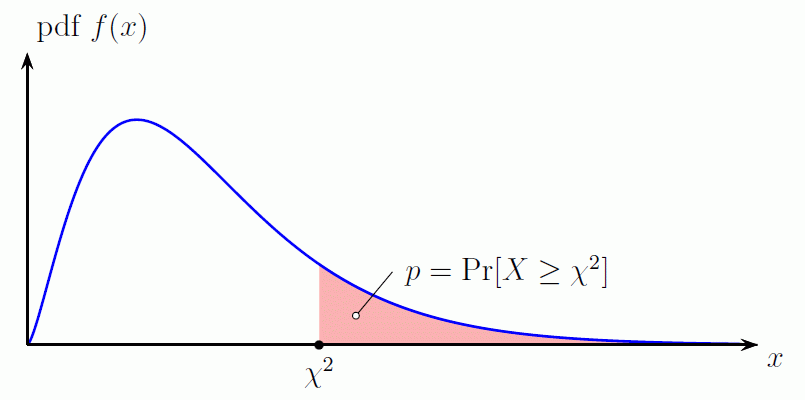
\includegraphics[width=0.7\textwidth]{images/spi/chisquare-pvalue}

\caption{Funkce hustoty (PDF) chí kvadrát rozdělení.}

\end{figure}

Test dobré shody je takzvaný neparametrický test, a tedy takový, že
nemusíme při jeho počítání vědět, jaké rozdělení má zkoumaná veličina.
Naší úlohou je určit za použití $\chi^{2}$~(\textit{\glqq Chí``})
testu dobré shody, zda odchylka odhadnuté hodnoty od té skutečně naměřené
vznikla jen náhodně nebo zda byl odhad špatný.

Mějme hodnoty pravděpodobnosti $p_{1},\ldots,p_{k}$ se kterými nastávají
jednotlivé výsledky náhodného pokusu o $k$ možných výsledcích. na
základě pozorování četností $n_{1},\ldots,n_{k}$ výsledků při $n$
nezávislých opakování pokusu.

Testujeme hypotézu
\[
H_{0}:\,p_{1}=p_{1}^{0};\,p_{2}=p_{2}^{0}\ldots;\,p_{k}=p_{k}^{0}
\]
proti
\[
H_{1}:\,p_{j}\neq p_{j}^{0}\,\,\text{alespoň pro jedno}\,\,j
\]
kde $p_{1}^{0}\ldots p_{k}^{0}\in\left(0,1\right),\,\sum_{j}p_{j}^{0}=1$
jsou daná čísla. Použijeme statistiku
\[
\chi^{2}={\displaystyle \sum_{j=1}^{k}\frac{\left(n_{j}-o_{j}\right)^{2}}{o_{j}}}
\]
kde $o_{j}=np_{j}^{0}$, \glqq$n$ `` je naměřená skutečnost a \glqq$o$ ``
je teoretický odhad. Za předpokladu, že $o_{j}>5$ a všechna $j=1,\ldots,k$,
zamítáme hypotézu $H_{0}$ na hladině významnosti $\alpha$, pokud
\[
\chi^{2}>\chi_{1-\alpha}^{2}\left(k-1\right)
\]
kde $\chi^{2}>\chi_{1-\alpha}^{2}\left(k-1\right)$ je $\left(1-\alpha\right)$-kvantil
Chí rozdělení.
\begin{flushright}
\cite{Friesl-2014}
\par\end{flushright}

\section{Test nezávislosti: Runs above/below the mean~\texorpdfstring{\faGraduationCap}{(*)}}

{

\exhyphenpenalty=10\hyphenpenalty=10

\marginpar{\textit{\textcolor{purple}{Testujeme }}\textbf{\textit{\textcolor{purple}{vzájemnou
nezávislost}}}\textit{\textcolor{purple}{{} náhodných veličin.}}}

}

Mějme náhodné proměnné $X_{1},\,X_{2},\ldots,X_{n}$ a předpokládejme,
že polovina prvků bude mít nižší hodnotu než $\mu$ („bellow/pod $\mu$“)
a polovina vyšší hodnotu („above/nad $\mu$“), tedy:
\begin{align*}
P\left(X_{i}=\mu\right) & =0\\
P\left(X_{i}<\mu\right) & =P\left(X_{i}>\mu\right)=\nicefrac{1}{2}
\end{align*}
Dále mějme hodnoty $R_{i}$ a $N_{n}$:
\begin{itemize}
\item $R_{i}=1$ pokud se hodnota v $i$-tém prvku mění z \glqq nad`` na
\glqq pod`` nebo obráceně;
\item $R_{i}=0$ pokud jsou hodnoty v $i$-tém prvku a v prvku předchozím
obě \glqq nad`` nebo obě \glqq pod``;
\item $N_{n}$ je počet míst, kde se takto mění hodnota, tedy $N_{n}=\sum_{i}R_{i}$.
\end{itemize}
Pokud jsou $X_{1},\,X_{2},\ldots,X_{n}$ skutečně nezávislé, pak počet
běhů pod/nad $\mu$ (při vysokých $n$) by měl odpovídat přibližně
tomuto normálnímu rozdělení:
\[
N_{n}=N\left(\mu=\frac{n+1}{2},\,\sigma^{2}=\frac{n-1}{4}\right)
\]
 a test nezávislost probíhá tímto způsobem:
\begin{enumerate}
\item Vypočteme $N_{n}$;
\item vypočteme $Z_{n}=\frac{N_{n}-E\left(N_{n}\right)}{\sigma=\sqrt{varN_{n}}}$;
\item porovnáme, zda $Z_{n}$ patří do intervalu normálního rozdělení (nulová
hypotéza je, že tam patří).
\end{enumerate}
\begin{flushright}
{[}\href{https://fit-wiki.cz/\%C5\%A1kola/p\%C5\%99edm\%C4\%9Bty/mi-spi/spi_szz/spi_szz_okruh_8}{FitWiki/spi\_szz\_okruh\_8}~\faLock{]}
\par\end{flushright}

\pagebreak{}

\part{Markovovy řetězce s~diskrétním a~spojitým časem a~jejich limitní
vlastnosti~(III.~okruh)\label{part:-SPI:-Markovsk=0000E9}}

\begin{tcolorbox}[title=\faWarning~Hlášení chyb ve třetím okruhu, colback=yellow!10, colframe=black!75!black, colbacktitle=yellow, coltitle=black, fonttitle=\bfseries]
\begin{flushleft}
Chyby a nedostatky v této sekci, prosím, hlaste na~\href{https://fit-wiki.cz/\%C5\%A1kola/p\%C5\%99edm\%C4\%9Bty/mi-spi/spi_szz/2017/spi_szz_okruh_3}{https://fit-wiki.cz/škola/předměty/mi-spi/spi\_szz/2017/spi\_szz\_okruh\_3}.
\par\end{flushleft}

\end{tcolorbox}

\textbf{Užitečné zdroje a odkazy:}
\begin{itemize}
\item \textbf{Hlavní zdroj pro tento okruh:} \href{https://docs.google.com/document/d/106a4c7arU0t8JJMneHMWMEqarFDHsve3twnhCMC4QnA/edit}{docs.google.com/.../...MC4QnA/edit}
\item Poissonův proces na Khan Academy: \href{https://www.khanacademy.org/math/statistics-probability/random-variables-stats-library/poisson-distribution/v/poisson-process-1}{www.khanacademy.org/.../poisson-process-1}
\item Vysvětlení MC od PatrickMJT: \href{https://www.youtube.com/watch\%3Fv\%3DuvYTGEZQTEs}{www.youtube.com/watch?v=uvYTGEZQTEs}
\item Poissonův proces od PatrickMJT: \href{https://www.youtube.com/watch\%3Fv\%3DFk02TW6reiA}{www.youtube.com/watch?v=Fk02TW6reiA}
\end{itemize}
\begin{tcolorbox}[colback=gray!10, colframe=black!30!black!50, colbacktitle=gray!15, coltitle=black, fonttitle=\bfseries]
\begin{flushleft}
Tématem se zabývají přednášky 9, 10, 11, 12, 13, 14, 15 a 16.
\par\end{flushleft}

\end{tcolorbox}

\section{tl;dr}

Rozlišujeme tyto základní pojmy:
\begin{itemize}
\item \textbf{\textcolor{purple}{\uline{Náhodný~proces}}} Soustava reálných
náhodných veličin indexovaná nejčastěji časem.
\item \textbf{\textcolor{purple}{\uline{Poissonův proces}}} Poissonův
proces je náhodný proces, který je \textbf{čítací, homogenní}\footnote{Jeho charakteristiky se v čase nemění.}
a \textbf{bez paměti}. Používáme jej pro modelování výskytu nějakých
událostí, které nastávají náhodně s určitou intenzitou $\lambda$
– výskyt zemětřesení, počet autonehod apod.
\item \textbf{\textcolor{purple}{\uline{Markovův řetězec}}} Markovův
řetězec je náhodný proces, který splňuje Markovovu podmínku\footnote{Proces je bez paměti.}.
\end{itemize}
\begin{center}
\colorbox{lightblue}{\textit{Markovův řetězec se spojitým časem }\textbf{\textit{je}}\textit{
}\textbf{\textit{časován}}\textit{ Poissonovým procesem.}}
\par\end{center}

\section{Náhodný proces}
\begin{center}
{\fboxsep 10pt\shadowbox{\begin{minipage}[c]{0.9\columnwidth}%
\textbf{\uline{Definice}}

Mějme pravděpodobnostní prostor ${\mathcal{E}=\left(\Omega,\,\EuScript{F},\,P\right)}$
(viz~\nameref{subsec:Pravd=00011Bpodobnostn=0000ED-prostor-()}~na~straně~\pageref{subsec:Pravd=00011Bpodobnostn=0000ED-prostor-()})
a množinu $T\subset\mathbb{R}$. Náhodným procesem pak nazýváme množinu
$\left\{ X_{t},\,t\in T\right\} $ (nebo také zapsáno jako $\left\{ X\left(t\right)|t\in T\right\} $),
kde $X_{t}$ jsou náhodné veličiny z~$\left(\Omega,\,\EuScript{F},\,P\right)$.
Prvky množiny $T$ se obvykle interpretují jako čas. Rozlišujeme procesy
s~diskrétním časem kde $T$ jsou celá číslo a procesy se spojitým
časem kde $T$ je interval reálných čísel. Jedná se tedy o \textbf{indexovanou
soustavu náhodných veličin}. Obecně platí, že dvě veličiny $X\left(t_{1}\right),X\left(t_{2}\right)$
pro různá $t_{1},t_{2}$ jsou nezávislé (jedná se o dvě veličiny v~různém
čase).

Náhodný proces můžeme definovat také jako zobrazení, které prvkům
z $T$ (jednotlivým \glqq časům``) přiřazuje nějaké $\mathbb{R}$.%
\end{minipage}}}
\par\end{center}

Náhodný proces, též stochastický proces\footnote{Stochastický (z řec. \textit{stochastiké techné}, umění uhádnout,
trefit se) znamená náhodný, nahodilý. Protikladem je deterministický.}, si lze představit jako zobecnění pojmů náhodná veličina a~náhodný
vektor. Zatímco výsledkem realizace náhodné veličiny je jedno číslo,
např.~výsledek hodu kostkou, je \textbf{realizací náhodného procesu
funkce nebo řada}.
\begin{flushright}
{[}\faWikipediaW~\href{https://cs.wikipedia.org/wiki/N\%C3\%A1hodn\%C3\%BD_proces}{CsWiki/Náhodný\_proces}{]}
\par\end{flushright}

Náhodným procesem, bez ohledu na formální matematickou definici, rozumíme
\textbf{soustavu náhodných veličin}, indexovaných diskrétním nebo
spojitým parametrem, který se často označuje jako čas.
\begin{flushright}
{[}\href{http://portal.matematickabiologie.cz/index.php\%3Fpg\%3Danalyza-a-modelovani-dynamickych-biologickych-dat--vybrane-kapitoly-z-matematickeho-modelovani--poissonuv-proces--definice-poissonova-procesu}{mamematickabiologie.cz}{]}
\par\end{flushright}

Náhodný proces je \textbf{zobrazení} $P:\,T\rightarrow S$, které
hodnotě $t\subset T$, kterou je nejčastěji čas, přiřazuje náhodný
jev, nejčastěji náhodnou veličinu. Pro minulé časové okamžiky zpravidla
víme, v jakém stavu proces byl, jaká byla historie procesu. Pro budoucí
okamžiky stav procesu neznáme a pokládáme jej za náhodný jev. Většinu
dějů \glqq ze života`` lze modelovat jako náhodné procesy.

\textbf{\textcolor{purple}{\uline{Homogenní náhodný proces}}} je
takový, jehož pravděpodobnostní charakteristiky se v čase nemění.
Tedy například pravděpodobnost, že dojde k události během minutového
intervalu, nezávisí na tom, kde je tento interval umístěn na časové
ose (tj. např. na tom, kolik je zrovna hodin nebo které je roční období).

\textbf{\textcolor{purple}{\uline{Čítací proces}}} je náhodný proces,
který je \textbf{tvořen událostmi stejného typ}u. Poněvadž všechny
události jsou stejné, je na čítacím procesu zajímavé pouze to, jak
jsou události rozloženy v čase, tedy např. kolik událostí nastalo
v závislosti na čase. Příklady čítacích procesů: Příchody zákazníků
do obchodu, otřesy zemské kůry, poruchy stroje.

Čítací proces $\left\{ N\left(t\right),\,t\geq0\right\} $ musí splňovat:
\begin{enumerate}
\item $N\left(t\right)\geq0$;
\item $N\left(t\right)$ jsou celá čísla;
\item $N\left(s\right)\leq N\left(t\right)$ pro každé $s<t$ (čítací proces
je neklesající);
\item Pro $s<t$ je $N\left(t\right)-N\left(s\right)$ počet událostí, které
nastaly v intervalu $\left(s,\,t\right\rangle $.
\end{enumerate}
\textbf{\textcolor{purple}{\uline{Čítací proces}}} \textbf{\textcolor{purple}{\uline{bez
paměti}}} je takový, kde budoucí výskyt události je stochasticky nezávislý
na předchozí historii procesu. To mimo jiné znamená, že znalost historie
procesu je pro předpovídání budoucího průběhu zcela bezcenná. Příklad:
opakovaně házíme kostkou, stavem procesu je počet bodů v naposledy
provedeném hodu. Tento proces je homogenní a bez paměti. Příkladem
čítacího procesu bez paměti je např. Poissonův proces.
\begin{flushright}
{[}\href{https://fit-wiki.cz/\%C5\%A1kola/p\%C5\%99edm\%C4\%9Bty/mi-spi/spi_szz/spi_szz_okruh_3}{FitWiki/.../spi\_szz\_okruh\_3}~\faLock{]}
\par\end{flushright}

\section{Poissonův proces~\texorpdfstring{\faGraduationCap}{(*)}}

\subsection{Úvod a motivace}
\begin{center}
{\fboxsep 10pt\fbox{\begin{minipage}[c]{0.9\columnwidth}%
\textbf{\uline{Příklad}}

Probíhá nějaký časově souvislý děj (např. emise částic), každý bod
$t$ v Poissonově procesu značí naše podívání se na měřicí přístroj
emisí a zapsání hodnoty $N\left(t\right)$ na papír. Počet emisí mezi
dvěma časovými úseky je vždy nezávislý na ostatních úsecích. Počet
naměřených emisí závisí jenom na délce úseku a ne na jeho umístění.
Emise v čase jsou vždy rovnoměrně distribuovány. Celý proces má Poissonovo
rozdělení, rozdělení intervalů mezi událostmi je exponenciální.
\begin{flushright}
{[}\href{https://fit-wiki.cz/\%C5\%A1kola/p\%C5\%99edm\%C4\%9Bty/mi-spi/spi_szz/spi_szz_okruh_3}{FitWiki/.../spi\_szz\_okruh\_3}~\faLock{]}
\par\end{flushright}%
\end{minipage}}}
\par\end{center}

Poissonův proces je náhodný proces, který je čítací, homogenní a bez
paměti. Tyto tři vlastnosti definují Poissonův proces jednoznačně
až na jediný parametr, totiž jeho intenzitu (průměrný počet událostí
za jednotku času). Jinými slovy, dva Poissonovy procesy jsou stejné
právě tehdy, když mají stejnou intenzitu. 
\begin{flushright}
{[}\href{https://fit-wiki.cz/\%C5\%A1kola/p\%C5\%99edm\%C4\%9Bty/mi-spi/spi_szz/spi_szz_okruh_3}{FitWiki/.../spi\_szz\_okruh\_3}~\faLock{]}
\par\end{flushright}

Poissonův proces je vhodným statistickým modelem např. pro
\begin{itemize}
\item radioaktivní rozpad částic;
\item počet telefonních hovorů;
\item požadavky zobrazení dokumentu na webu.
\end{itemize}
Jedná se o náhodný proces se \textbf{spojitým časem} a diskrétní množinou
stavů (nezáporná celá čísla). S~tématem dále souvisí \nameref{subsec:Poissonovo-rozd=00011Blen=0000ED-/diskr=0000E9tn=0000ED/}~na~straně~\pageref{subsec:Poissonovo-rozd=00011Blen=0000ED-/diskr=0000E9tn=0000ED/}.
Poissonův proces má dvě možné formální definice\footnote{V tomto dokumentu je nejprve uvedená II definice, a pak I. V přednáškách
je tomu přesně opačně – avšak II definice je subjektivně srozumitelnější.}.

\subsection{Formální definice pomocí nezávislých přírůstků (II.~definice)}

Poissonův proces $N=\left\{ N\left(t\right),\,t\geq0\right\} $ je
stochastický čítací proces se spojitým časem a~intenzitou $\lambda,\,\lambda>0$,
který nabývá hodnot z $S=\left\{ 0,\,1,\,2,\ldots\right\} $. Platí
pro něj následující vlastnosti:
\begin{enumerate}
\item $N\left(0\right)=0$, $s<t\Rightarrow N\left(s\right)\leq N\left(t\right)$;
\item má nezávislé přírůstky;
\item počet událostí v jakémkoli intervalu délky $t$ je Poissonovská náhodná
proměnná s~průměrem (střední hodnotou)~$\lambda t$\footnote{Říká, kolik průměrně nastává událostí za časový okamžik.}.
Tedy $N\left(s+t\right)-N\left(s\right)\sim\text{Poisson}\left(\lambda t\right)$.
\end{enumerate}
\begin{flushright}
{[}\faWikipediaW~\href{https://en.wikipedia.org/wiki/Poisson_point_process}{EnWiki/Poisson\_point\_process},
Lecture12/Slide45{]}
\par\end{flushright}
\begin{enumerate}
\item Vynulujeme counter, nezačínáme ve vzduchoprázdnu.
\item Všechny přírůstky (příchody; schody na křivce) jsou nezávislé. Např.
je jedno, zda padne panna nebo orel, když předtím padla panna nebo
orel.
\item Přírůstky jsou stacionární. Mějme nějaký interval pevné délky $\left\langle s,\,t\right\rangle $
a šoupejme s ním po ose $\left\langle s+u,\,t+u\right\rangle $. Procesu
se stacionárními přírůstky má všude stejné statistické charakteristiky
– nestane se tedy, že jeden interval bude rozdělený pomocí Gaussovy
distribuce a druhý pomocí Poissonovy distribuce.
\end{enumerate}
\begin{flushright}
{[}\href{https://docs.google.com/document/d/106a4c7arU0t8JJMneHMWMEqarFDHsve3twnhCMC4QnA/edit\#}{docs.google.com...}{]}
\par\end{flushright}

\begin{figure}[H]
\centering

\includegraphics[width=0.9\textwidth]{\string"images/spi/poisson process nezavisle prirustky\string".png}

\caption{Nezávislé přírůstky u Poissonova procesu}
\end{figure}


\subsection{Formální definice pomocí exponenciálních časů příchodů (I.~definice)}

V této definici zkoumáme čas mezi jednotlivými příchody (na obrázku
je čas mezi příchody značen jako $t_{k}$). Čas mezi příchody je rozdělený
exponenciálně. 

Více o exponenciálním rozdělení v kapitole \nameref{subsec:Exponenci=0000E1ln=0000ED-rozd=00011Blen=0000ED-/spojit=0000E9}~na~straně~\pageref{subsec:Exponenci=0000E1ln=0000ED-rozd=00011Blen=0000ED-/spojit=0000E9}.
\begin{flushright}
{[}\href{https://docs.google.com/document/d/106a4c7arU0t8JJMneHMWMEqarFDHsve3twnhCMC4QnA/edit\#}{docs.google.com...},
Lecture12/Slide04{]}
\par\end{flushright}

\begin{figure}[H]
\centering

\includegraphics[width=1\textwidth]{\string"images/spi/poisson process exponencialni prichody\string".png}

\caption{Exponenciální časy příchodů v Poissonově procesu. $T_{k}$ značí příchod
$k$-tého zákazníka, $t_{k}\sim\text{Exp}\left(\lambda\right)$. ~{[}Lecture12/Slide04{]}}
\end{figure}


\subsubsection{Čas příchodu}

Čas příchodů, někdy též doba čekání, $n$-té události je suma prvních
$n$ dob trvání.
\[
T_{n}=t_{1}+t_{2}+\ldots+t_{n}
\]

Jednoduše přesný okamžik, kdy nastane daný jev. Např.: Měříme čas
od $T_{0}=12:00$, v~$T_{1}=12:02$ nastane první událost (čekali
jsme 2 minuty, $t_{1}=2$), další událost nastane $T_{2}=12:05$,
tedy $t_{2}=3$ resp. $T_{2}=t_{1}+t_{2}=2+3\sim12:05$.

Vysvětlení $N\left(s\right)=\max\left\{ n:\,T_{n}\leq s\right\} $
z obrázku výše. Tady nejde o nic jiného, než o to, že pokud si někde
v čase zastavíme (zarážka s na x-ové ose) a ohlédneme se za sebe (tj.
směrem k nule), vidíme všechny \glqq Téčka`` jako např. korálky na
niti. Tyto korálky jsou očíslovány vzestupně od $0$ po $n$. Vezmeme
poslední korálek a podíváme se jaké má číslo $n$. Toto číslo je shodou
okolností také $N\left(s\right)$ neboli počet příchodů (korálků)
od počátku. Na slajdu je $\max\left\{ 1,2,3,4\right\} $ což je vcelku
logicky $4$. Neboli číslo posledního korálku, neboli celkový počet
příchodů v čase $s$.
\begin{flushright}
{[}\href{https://docs.google.com/document/d/106a4c7arU0t8JJMneHMWMEqarFDHsve3twnhCMC4QnA/edit\#}{docs.google.com...}{]}
\par\end{flushright}

\section{Markovovy řetězce s diskrétním parametrem (DTMC)~\texorpdfstring{\faGraduationCap}{(*)}}

\subsection{Definice Markovova řetězce}

{

\exhyphenpenalty=10\hyphenpenalty=10

\marginpar{\protect\begin{flushleft}
\textit{\textcolor{purple}{\glqq Posloupnost náhodných veličin, která
splňuje Markovovu podmínku.``}}\protect
\par\end{flushleft}}

}
\begin{center}
{\fboxsep 10pt\shadowbox{\begin{minipage}[c]{0.9\columnwidth}%
\textbf{\uline{Definice}}

Posloupnost $X=\left\{ X_{0},X_{1},\ldots\right\} $ náhodných veličin
nabývajících hodnot z nejvíce spočetné množiny stavů $S$, která splňuje
(ta posloupnost) Markovskou podmínku, se nazývá Markovský řetězec
s diskrétním časem.

Markovův řetězec je plně definován
\begin{itemize}
\item množinou stavů $S$;
\item vektorem počátečního rozdělení (někde musíme začít);
\item maticí přechodů $P$.
\end{itemize}
%
\end{minipage}}}
\par\end{center}

Markovův řetězec \textbf{popisuje} obvykle \textbf{diskrétní náhodný
proces}, pro který platí, že pravděpodobnosti přechodu do následujícího
stavu závisejí \textbf{pouze na~současném stavu}, ne na~předchozích
stavech (viz~\nameref{subsec:Markovova-podm=0000EDnka}). Tato tzv.~Markovova
vlastnost dovoluje proces znázornit stavovým diagramem, kde z každého
stavu (uzlu grafu) vycházejí hrany možných přechodů do dalšího stavu
s~připsanou pravděpodobností.

Markovův řetězec můžeme zapsat (znázornit)
\begin{itemize}
\item stavovým diagramem;
\item maticí přechodů $P$.
\end{itemize}
\begin{flushright}
{[}\faWikipediaW~\href{https://cs.wikipedia.org/wiki/Markov\%C5\%AFv_\%C5\%99et\%C4\%9Bzec}{CsWiki/Markovův\_řetězec}{]}
\par\end{flushright}

Co to ale je ten \glqq diskrétní čas``? Představte si, že čas jako
takový vlastně vůbec neřešíte. Máte někde hodiny, které vám pravidelně
odbíjejí impuls. Kdykoli přijde tento impuls zvýšíte $n$ o jedničku
a tím přejdete do dalšího stavu. Čas je v tomto případě diskrétní
(jakoby přesně oddělený, pravidelný). 

Co když ale nebudu mít takové hodiny, které budou pravidelně odbíjet
impuls. Co když tento impuls bude nastávat zcela náhodně tzn. v různých
časových intervalech? Potom budu potřebovat Markovův řetězec se spojitým
časem (CTMC):
\begin{flushright}
{[}\href{https://docs.google.com/document/d/106a4c7arU0t8JJMneHMWMEqarFDHsve3twnhCMC4QnA/edit\#}{docs.google.com...}{]}
\par\end{flushright}

\subsection{Vlastnosti Markovova řetězce}
\begin{itemize}
\item Markovovy řetězce dělíme na \textbf{\textcolor{purple}{\uline{homogenní}}}
a \textbf{\textcolor{purple}{\uline{nehomogenní}}}. Pro homogenní
řetězec platí, že $p_{ij}\left(n\right)$ nezávisí na $n$, nehomogenní
závisí. Pro homogenní řetězec tedy platí
\[
P\left(X_{n+1}=j|X_{n}=i\right)=P\left(X_{1}=j|X_{0}=i\right)
\]
(pravděpodobnost přechodu $i\rightarrow j$ nezávisí na tom, jestli
právě začínáme, nebo už jsme předtím něco nachodili).
\item Markovův řetězec je \textbf{ireducibilní}, pokud jeho stavový prostor
umožňuje dostat se z libovolného stavu do jiného (ne nutně v jednom
kroku).
\end{itemize}

\subsection{Markovova podmínka (vlastnost)\label{subsec:Markovova-podm=0000EDnka}}

{

\exhyphenpenalty=10\hyphenpenalty=10

\marginpar{\protect\begin{flushleft}
\textit{\textcolor{purple}{\glqq}}\textbf{\textit{\textcolor{purple}{Bez
paměti}}}\textit{\textcolor{purple}{; nezajímají nás dříve navštívené
stavy.``}}\protect
\par\end{flushleft}}

}
\begin{center}
{\fboxsep 10pt\fbox{\begin{minipage}[c]{0.7\columnwidth}%
\textbf{Poznámka k notaci:}
\begin{itemize}
\item Čárka »,« v Markovově podmínce znamená \glqq AND``. 
\item $X_{n}=s_{i}$ říká \glqq$i$ -tý stav v $n$-tém kroku``
\end{itemize}
%
\end{minipage}}}
\par\end{center}

Říká, že pravděpodobnost budoucích stavů je plně určena současným
stavem bez ohledu na minulé stavy
\[
P\left(X_{n}=s_{j}|X_{0}=s_{0},\,X_{1}=s_{1},\,\ldots,\,X_{n-1}=s_{i}\right)=\boxed{P\left(X_{n}=s_{j}|X_{n-1}=s_{i}\right)=P_{ij}}
\]

\begin{siderules}\colorbox{blue!20}{\faLightbulbO}~V kroku $0$
jsme byli ve stavu $s_{0}$, v~kroku $1$ jsme byli ve stavu $s_{1}$\ldots{}
nyní jsme v~kroku $n-1$ ve stavu $s_{i}$ a ptáme se, jaká je pravděpodobnost,
že z~tohoto stavu opravu skočíme do~stavu $s_{j}$. Tato pravděpodobnost
je naprosto stejná, jak kdybychom celou historii neznali: tj. víme
jen, že jsme v kroku $n-1$ a~v~následujícím chceme do stavu $s_{j}$.\end{siderules}

V každém stavu procesu je pravděpodobnost navštívení dalších stavů
nezávislá na dříve navštívených stavech. Chování je tedy \textbf{\textcolor{purple}{\uline{bezpaměťové}}}\textbf{.}
\begin{flushright}
{[}Lecture9/Slide05{]}
\par\end{flushright}

\subsection{Matice přechodů, přechodová matice\label{subsec:Matice-p=000159echod=00016F,-p=000159echodov=0000E1}}

Mějme posloupnost diskrétních náhodných veličin $X_{0},\,X_{1},\ldots,X_{n}$
s hodnotami ze spočetné množiny stavů $S=\left\{ s_{1},\,s_{2},\ldots,s_{n}\right\} $.

Pravděpodobnost přechodu ze stavu $i$ do stavu $j$ v jednom kroku
zapíšeme jako
\[
P_{i,j}=p\left(i,\,j\right)=P\left(X_{n+1}=s_{j}|X_{n}=s_{i}\right)
\]

(Jsme ve stavu $\text{␣}|s_{i}$ a chceme do $s_{j}|\text{␣}$\footnote{V matici $i$ značí řádky a $j$ sloupce.}).
Zároveň můžeme sestavit \textbf{matici přechodů}\footnote{Ta se někdy značí jako $\Pi$ a její mocniny jako $\Pi^{2}\ldots$.}\textbf{
}(matice s~přechodovými pravděpodobnostmi; \textit{transition~}\textbf{\textit{p}}\textit{robability~matrix})

\[
\begin{array}{ccc}
 & \begin{array}{ccc}
s_{j=1} & \cdots & s_{j=n}\end{array} & \leftarrow\text{následující stav}\\
P=\begin{array}{c}
s_{i=1}\\
\vdots\\
s_{i=n}
\end{array} & \begin{pmatrix}p_{11} & \cdots & p_{1n}\\
\vdots & \ddots & \vdots\\
p_{n1} & \cdots & p_{nn}
\end{pmatrix}\\
\overset{\nearrow}{\text{současný stav}}
\end{array}
\]

pro tu musí platit, že
\[
\forall i=1,\ldots,n:\,\sum_{j=1}^{n}p_{ij}=1
\]
tedy že součet řádků se rovná $1$ (matice přechodů je stochastická).

Dále platí, že prvek $ij$ matice $P^{n}$ říká pravděpodobnost $p_{ij}^{n}$
(tzv.~\textbf{vícekroková pravděpodobnost}), že Markovův řetězec
začínající ve stavu $s_{i}$ bude ve~stavu $s_{j}$ v $n$ krocích.
Tedy platí
\[
P\left(X_{n}=s_{j}|X_{0}=s_{i}\right)=P_{ij}^{n}
\]

\begin{flushright}
{[}Lecture9/Slide05+07{]}
\par\end{flushright}

Vysvětlení: Chceme se dostat do stavu $s_{j}$ v kroku $n$ a vycházíme
ze stavu $s_{i}$, což je krok $0$. Potřebujeme tedy matici přechodů,
která je $n$-krát vynásobená sama sebou. Téma dále pokračuje kapitolou
\nameref{subsec:Kolmogorov-Chapman-rovnice}~na~straně~\pageref{subsec:Kolmogorov-Chapman-rovnice}.

\subsection{Reprezentace diagramem}

\begin{figure}[H]
\centering

\includegraphics[width=0.35\textwidth]{\string"images/spi/Markovkate 01\string".pdf}

\caption{Jednoduchý diskrétní Markovův řetězec se dvěma stavy. Obrázek říká,
že je-li systém ve stavu \colorbox{lightgray}{E}, přejde s pravděpodobností
$0,7$ do~stavu \colorbox{lightgray}{A}, kdežto s~pravděpodobností
$0,3$ zůstane ve~stavu \colorbox{lightgray}{E}. Podobně po~stavu
\colorbox{lightgray}{A} bude s~pravděpodobností $0,4$ následovat
stav \colorbox{lightgray}{E}, kdežto s~pravděpodobností $0,6$ systém
zůstane ve~stavu \colorbox{lightgray}{A}. Chování takového systému
je tedy „bezpaměťové“: není potřeba si pamatovat historii, stačí pouze
aktuální stav. Reprezentací takového systému tedy může být konečný
automat.~{[}\faWikipediaW~\protect\href{https://cs.wikipedia.org/wiki/Markov\%C5\%AFv_\%C5\%99et\%C4\%9Bzec}{CsWiki/Markovův\_řetězec}{]}}

\end{figure}


\subsection{Absorpční řetězce}
\begin{center}
{\fboxsep 10pt\shadowbox{\begin{minipage}[c]{0.9\columnwidth}%
\textbf{\uline{Druhy stavů}}

Po opuštění nějakého stavu definujeme pravděpodobnost, že se systém
do tohoto stavu vrátí, následovně:
\begin{itemize}
\item Je-li $p<1$ je stav \textbf{tranzientní};
\item Je li $p=1$ je stav \textbf{rekurentní} (přes den lítám po tranzientních
stavech, ale večer se vždy dostanu do postele);
\item Stav, který nemůžeme opustit, je stav \textbf{absorpční}.
\end{itemize}
%
\end{minipage}}}
\par\end{center}

Absorpční řetězce jsou takové řetězce, které \textbf{obsahují} mimo
stavy tranzientní (přechodové) i~\textbf{stavy absorpční} (pro stav
$s_{i}\in S$ platí $P_{ii}=1$). Tzn., že pravděpodobnost setrvání
v takovém stavu je rovna~$1$\footnote{Tento stav je tedy \textbf{nemožné opustit.}}. 

Stačí, aby v řetězci existoval alespoň jeden takovýto stav, avšak
je nutné, aby bylo do~tohoto stavu možné dojít.
\begin{flushright}
{[}Lecture9/Slide13{]}
\par\end{flushright}

Máme-li konečně mnoho neabsorpčních stavů, je pravděpodobnost, že
bude proces absorbován~$1$, platí tedy
\[
\lim_{n\rightarrow\infty}=Q^{n}=0
\]

\begin{flushright}
{[}Lecture9/Slide14{]}
\par\end{flushright}

\begin{figure}[H]
\centering

\includegraphics[scale=0.65]{images/spi/absorbing_markov}

\caption{Ukázka absorpčního Markovova řetězce. Z rekurentního stavu \colorbox{lightgray}{A}
již není cesty zpět.}
\end{figure}

Matice přechodů (\textit{transition~matrix}; kanonický\footnote{Forma objektu, ve které může být objekt jednoznačně prezentován.}
zápis matice) absorpčního Markovova řetězce s $r$ absorpčními stavy
a~$t=\ell-r$ neabsorpčními stavy má tvar\footnote{Jedná se o standardní čtvercovou matici, vnitřní čáry jen naznačují,
že je matice \glqq virtuálně`` rozdělena do čtyř submatic.}

\[
\begin{array}{cc}
 & \begin{array}{cc}
\text{TR} & \text{ABS}\end{array}\\
P=\begin{array}{c}
\text{TR}\\
\text{ABS}
\end{array} & \left(\begin{array}{c|c}
Q & R\\
\hline 0 & 1
\end{array}\right)
\end{array}
\]
kde
\begin{itemize}
\item $P$ je matice přechodů;
\item $Q$ jsou tranzientní stavy ($Q$ má velikost $t\times t$);
\item $R$ jsou absorpční stavy;
\item $0$ je nulová matice\footnote{Obsahuje samé nuly.} velikosti $r\times t$;
\item $1$ ($I$) je jednotková matice velikosti $r\times r$, která vyjadřuje,
že z těchto stavů není možné uniknout.
\end{itemize}
\begin{flushright}
{[}Lecture9/Slide14{]}
\par\end{flushright}

Pravděpodobnost, že se dostaneme do stavu $s_{j}$ pomocí $n$ kroků
ze stavu $s_{i}$ spočteme mocněním matice $P$
\[
P^{n}=\begin{pmatrix}Q^{n} & R^{\left(n\right)}\\
0 & 1
\end{pmatrix}
\]
$Q^{n}$ zároveň dává pravděpodobnost, že po $n$ krocích \textbf{nebudeme}
v absorpčním stavu.

\subsubsection{Fundamentální matice absorpčního řetězce}

Fundamentální matice je matice ve tvaru
\[
N=\left(I-Q\right)^{-1}
\]
kde
\begin{itemize}
\item $I$ je jednotková matice;
\item $\mathcircumflex1$ značí inverzní matici.
\end{itemize}
Prvky fundamentální matice $N$ udávají, kolikrát se proces v průměru
ocitne v tranzientních stavech (tedy jimi proces projde).

$N_{i,j}=\mathbb{E}\left(\text{počet průchodů stavem j}|\text{začínáme ve stavu i}\right)$,
zároveň součet řádku je střední doba absorpce, pokud začínáme v určitém
stavu.

\subsubsection{Pravděpodobnostní matice}

Pravděpodobnost, že spadneme do absorpčního stavu \glqq$j$ ``,
začínáme-li v \glqq$i$ `` je
\[
B_{i,j}=\mathbb{P}\left(\text{pohlcení v }s_{j}|\text{start v }s_{i}\right)
\]

Matici $B$ vypočítáme jako
\[
B=N*R
\]

\begin{center}
(Nezapomeňme, že matice $B$ kopíruje označení sloupců a řádků z matice
přechodů $P$)
\par\end{center}

\section{Markovovy řetězce se spojitým parametrem (CTMC)~\texorpdfstring{\faGraduationCap}{(*)}}

\subsection{\texorpdfstring{\colorbox{blue!20}{\faLightbulbO}}{(!)}~Značení
matic CTMC}

{

\exhyphenpenalty=10\hyphenpenalty=10

\marginpar{\protect\begin{flushleft}
\textit{\textcolor{purple}{Můžeme převést: ${P_{t}\rightsquigarrow Q\rightsquigarrow U}$.}}\protect
\par\end{flushleft}}

}

Z DTMC známe jedinou matici $P$, ve které se nacházejí přechodové
pravděpodobnosti. V~CTMC používáme následující matice:

{\exhyphenpenalty=10\hyphenpenalty=10\marginpar{\protect\begin{flushleft}
\textit{\textcolor{purple}{$P_{t}$:~Matice funkcí.}}\protect
\par\end{flushleft}}}
\begin{itemize}
\item Matice $P_{t}$
\[
P_{t}=\begin{pmatrix}\cdots & \cdots\\
\cdots & \cdots
\end{pmatrix}\begin{array}{c}
=\sum1\\
=\sum1
\end{array}
\]
je \textbf{matice pravděpodobnosti přechodu} ze stavu $i$ do stavu
$j$ v čase $t$, tato matice je časovaná Poissonovým procesem. Platí,
že řádky matice se musí rovnat $1$. Prvky matice jsou nějaké \textbf{funkce}
(viz další sekci).
\item Matice $Q$
\[
Q=\begin{pmatrix}\cdots & \cdots\\
\cdots & \cdots
\end{pmatrix}\begin{array}{c}
=\sum0\\
=\sum0
\end{array}
\]
je \textbf{matice skokových intenzit} (anglicky \textit{jump rates}).
Prvky matice jsou \glqq lambdy`` – intenzity přeskoku (tedy $q\left(i,j\right)$).
Platí, že řádky matice se musí rovnat $0$, na~diagonále se nacházejí
záporné lambdy. Uveďme příklad
\[
Q=\begin{pmatrix}-2\lambda & \lambda & \lambda\\
\cdots & -\lambda & \lambda\\
\lambda & \cdots & -\lambda
\end{pmatrix}\begin{array}{c}
=0\\
=0\\
=0
\end{array}
\]
\item Matice $U$
\[
U=\begin{pmatrix}\cdots & \cdots\\
\cdots & \cdots
\end{pmatrix}
\]
je \textbf{matice diskrétních přechodových pravděpodobností v náhodném
čase $t$}. De facto odpovídá přechodové matici $P$ z DTMC (\textbf{\textcolor{red}{nikoliv}}
$P_{t}$!). Její prvky odpovídají
\[
u_{ij}=\left(U\right)_{ij}=\begin{cases}
\frac{\lambda_{ij}}{\lambda_{MAX}}=\frac{q\left(i,j\right)}{\lambda_{MAX}} & \text{pro\,}i\neq j\\
1+\frac{\lambda_{ij}}{\lambda_{MAX}} & \text{pro\,}i=j
\end{cases}
\]
kde $\lambda_{MAX}$ je největší součet odchozích skokových intenzit.
Touto maticí převedeme CTMC na DTMC.
\end{itemize}
{

\exhyphenpenalty=10\hyphenpenalty=10

\marginpar{\protect\begin{flushleft}
\textit{\textcolor{purple}{Rozlišujeme matice $Q,\,P_{t},\,U$.}}\protect
\par\end{flushleft}}

}

Matice $P_{t}$ a $Q$ (resp. a $U$) mezi sebou můžeme převádět (\glqq$'$ ``
značí derivaci):

\begin{align}
Q & =P_{t}'\left(t=0\right)\\
P_{t}' & =Q*P_{t}\\
P_{t}' & =P_{t}*Q
\end{align}
Rovnici $\left(2\right)$ nazýváme \glqq Kolmogorov's Backward Equation``,
rovnici $\left(3\right)$ nazýváme \glqq Kolmogorov's Forward Equation``.
Aby rovnice platily, musí být řetězec homogenní.
\begin{flushright}
{[}Lecture14/Slide32, CZ\_Cvičení09/Slide07{]}
\par\end{flushright}

\subsection{Definice}
\begin{center}
{\fboxsep 10pt\shadowbox{\begin{minipage}[c]{0.9\columnwidth}%
\textbf{\uline{Markovovy řetězce se spojitým parametrem}}

\smallskip{}

\begin{flushleft}
CTMC\footnote{Continuous-time Markov chain.} se spojitým parametrem
rozšiřují standardní DTMC\footnote{Discrete-time Markov chain.} s~diskrétním
parametrem o to, že nevíme, jak dlouho zůstaneme v~nějakém stavu.
\par\end{flushleft}
\begin{flushleft}
V každém časovém okamžiku se nacházím v nějakém stavu. S nějakou intenzitou
přechodu v každém časovém okamžiku chci svůj stav změnit. Kam skočím
udává pravděpodobnost přechodu. To znamená, že řešíme dvě věci: za
jak dlouho změníme stav (\textit{jump rate}; \textbf{intenzita~přechodu})
a kam půjdeme (\textbf{přechodová pravděpodobnost} je stejná jako
u MC s diskrétním parametrem). Kolmogorovovy rovnice dávají návod,
jak z \textit{jump rate} spočítat přechodovou pravděpodobnost. Pro
modelování \textit{jump rate} se dá s~úspěchem použít Poissonův proces. 
\par\end{flushleft}
\begin{flushright}
{[}\href{https://fit-wiki.cz/\%C5\%A1kola/p\%C5\%99edm\%C4\%9Bty/mi-spi/spi_szz/spi_szz_okruh_3}{FitWiki/.../spi\_szz\_okruh\_3}~\faLock{]}
\par\end{flushright}%
\end{minipage}}}
\par\end{center}

Mějme Poissonův proces $\left\{ N\left(t\right),\,t\geq0\right\} $
s~intenzitou $\lambda$ a Markovův řetězec s~\textbf{diskrétním
časem} $Y_{n}$ s přechodovými pravděpodobnostmi $u\left(i,\,j\right)$.
Předpokládejme, že $N\left(t\right)$ je nezávislý na $Y_{n}$, potom
\[
X_{t}=Y_{N\left(t\right)}
\]
je Markovův řetězec (někdy též Markovův proces) se \textbf{spojitým
časem}. V Markovově řetězci se spojitým časem neexistují stavy periodické.
\begin{flushright}
{[}Lecture14/Slide05{]}
\par\end{flushright}

CTMC je spojení DTMC s Poissonovým procesem pro časování skoků mezi
stavy. Jako důsledek máme CTMC, které skáče na základě svých přechodových
pravděpodobností $u\left(i,j\right)$\footnote{Přechodová pravděpodobnost je stejná jako u DTMC, jen se jinak značí.},
avšak vždy v čase příchodu $N\left(t\right)$. To pak značíme $p_{t}\left(i,j\right)$.
To jak často bude CTMC skákat je dáno intenzitou $\lambda$. Takže
například $3\times$ za minutu.

Nyní si ukážeme, jak vypadají přechodové pravděpodobnosti v praxi.
Mějme Poissonův proces
\begin{align*}
N\left(t\right)\sim\text{Poisson}\left(\lambda t\right)\\
P\left(N\left(t\right)=n\right)=\frac{\left(t\lambda\right)^{x}}{x!}\mathrm{e}^{-t\lambda}
\end{align*}
Poté pro \textbf{přechodovou pravděpodobnost CTMC}
\[
p_{t}\left(i,j\right)=P\left(X_{t}=j|X_{0}=i\right)
\]
platí
\begin{align*}
\boxed{p_{t}\left(i,j\right)} & =\sum_{n=0}^{\infty}P\left(N\left(t\right)=n,\,X_{t}=j|X_{0}=i\right)\\
 & =\ldots\\
 & =\boxed{\sum_{n=0}^{\infty}\frac{\left(t\lambda\right)^{x}}{x!}\mathrm{e}^{-t\lambda}u^{n}\left(i\,,j\right)}
\end{align*}
což je suma přes všechny možné počty kroků. Pokud je $i\neq j$, je
přechod v $0$ krocích nemožný, pokud $i=j$, je pravděpodobnost přechodu
$1$.
\begin{flushright}
{[}Lecture14/Slide06{]}
\par\end{flushright}

\subsection{Markovova podmínka pro CTMC}

$X_{t},\,t\geq0$ je CTMC pokud pro každý čas $0\leq s_{0}\leq s_{1},\,\ldots,\,s_{n}<s$
a jakýkoliv stav $i_{0},\,i_{1},\,\ldots,i_{n},\,i\,j$ (pro všechna
$n\geq1$) platí
\begin{align*}
P\left(X_{t+s}=j|X_{s}=i,\,X_{s_{n}}=i_{n},\,X_{s_{0}}=i_{0}\right)=\\
 & =P\left(X_{t+s}=j|X_{s}=i\right)\\
 & =\boxed{P\left(X_{t}=j|X_{0}=i\right)=p_{t}\left(i,j\right)}
\end{align*}

\begin{flushright}
{[}Lecture14/Slide04{]}
\par\end{flushright}

Pro srovnání připomeňme Markovovu podmínku pro DTMC
\[
P\left(X_{n}=s_{j}|X_{n-1}=s_{i}\right)=p\left(i,j\right)
\]
co se změnilo:
\begin{itemize}
\item nezačínáme v předchozím stavu ($n-1$), ale ve stavu $0$;
\item nejdeme do následujícího stavu ($n-1\rightarrow n$), ale do stavu
$0\rightarrow t$;
\item $p\left(i,j\right)$ se změnilo na $p_{t}\left(i,j\right)$.
\end{itemize}
\begin{flushright}
{[}Lecture9/Slide14{]}
\par\end{flushright}

Když jsme tedy ve stavu $n$, znamená to, že jsme akorát dostali impuls
a do tohoto stavu jsme se dostali ze stavu $n-1$. V~CTMC se však
nastaví čas na $0$. V~DTMC to neřešíme, zkrátka jsme v $n$. V DTMC
dále nastává impuls v diskrétním čase (pravidelně) a systém se přesouvá
do $n+1$ (zase čas jako takový neřeším, protože vím, že vždy přijde
impuls pravidelně). 

V CTMC je situace jiná. Protože nikdy nevíme kdy do dalšího stavu
přejdeme, označíme moment přechodu $t$, které ovšem může být pokaždé
různé. Jistě vás teď napadá otázka jak by se daly takovéto náhodné
časy modelovat. Nečekaně např. pomocí Poissonova procesu.
\begin{flushright}
{[}\href{https://docs.google.com/document/d/106a4c7arU0t8JJMneHMWMEqarFDHsve3twnhCMC4QnA/edit\#}{docs.google.com...}{]}
\par\end{flushright}

\subsection{Intenzita přechodu (Jump rate)}

{

\exhyphenpenalty=10\hyphenpenalty=10

\marginpar{\protect\begin{flushleft}
\colorbox{blue!20}{\faLightbulbO}~\textit{\textcolor{purple}{Intenzity
přechodu potřebujeme, abychom převedli CTMC na~DTMC.}}\protect
\par\end{flushleft}}

}

Představme si, že jsme v nějakém stavu. Poissonův proces má nějakou
intenzitu, např.~${\lambda=3}$ za vteřinu, aka v průměru mi za vteřinu
tiknou hodiny $3\times$. Když tiknou, tak skočím. Dejme tomu, že
mám dvě možnosti kam skočit – $j_{1}$ a $j_{2}$. Do~$j_{1}$ skočím
s~pravděpodobností $0,8$ a do $j_{2}$ s pravděpodobností $0,2$.
Intenzita se mi potom bude ředit dle daných pravděpodobností. Celkem
logicky pak budu do $j_{1}$ skákat častěji - s intenzitou $2,4$
a~do~$j_{2}$ méně často s intenzitou $0,6$. Tohle je tzv. Poisson
Process Thinning neboli \textbf{ředění Poissonova procesu}. 

\begin{figure}[H]
\centering

\includegraphics[width=0.7\textwidth]{\string"images/spi/Image 4\string".png}

\caption{Všimněte si, že v každé větvi mám pak úplně nový Poissonův proces
(jednoduše proto, že se mi změnila $\lambda$). Tyto dvě \glqq nové``
intenzity se nazývají jump rates neboli skokové intenzity a značí
se $q\left(i,j\right)$.}

\end{figure}

Jump rates jsou součiny $\lambda$ a přechodových pravděpodobností
\[
q\left(i,j\right)=\highlight{\lambda*u\left(i,j\right)},\,q\left(i.j\right)\in Q
\]

Zajímavé je pak to, že tyto nové intenzity jsou přesně tato derivace
(pro $j\neq i$): 

\begin{align*}
q\left(i,j\right) & =\left.\frac{\text{d}\,p_{t}\left(i,j\right)}{\text{d}t}\right|_{t=0}\\
 & =\ldots\\
 & =\lim_{h\rightarrow0^{+}}\frac{p_{h}\left(i,j\right)}{h}\\
 & =\lim_{h\rightarrow0^{+}}\lambda\mathrm{e}^{-h\lambda}u\left(i\,,j\right)\\
 & =\highlight{\lambda*u\left(i,j\right)}
\end{align*}
kde $p_{t}\left(i,j\right)\in P_{t}$.
\begin{flushright}
{[}\href{https://docs.google.com/document/d/106a4c7arU0t8JJMneHMWMEqarFDHsve3twnhCMC4QnA/edit\#}{docs.google.com...},
Lecture14/Slide12+16{]}
\par\end{flushright}

\section{Kolmogorov-Chapmanova rovnice~\texorpdfstring{\faGraduationCap}{(*)}\label{subsec:Kolmogorov-Chapman-rovnice}}

\subsection{Rovnice pro DTMC}

{

\exhyphenpenalty=10\hyphenpenalty=10

\marginpar{\protect\begin{flushleft}
\textit{\textcolor{purple}{Jaká je pravděpodobnost přechodu mezi dvěma
stavy v~určitém počtu kroků?}}\protect
\par\end{flushleft}}

}

Kapitola navazuje na~\nameref{subsec:Matice-p=000159echod=00016F,-p=000159echodov=0000E1}~na~straně~\pageref{subsec:Matice-p=000159echod=00016F,-p=000159echodov=0000E1}.

Zjistit pravděpodobnost přechodu v $n$-tém kroku zjistíme mocněním
matice přechodů $P$. Tento postup je však zdlouhavý pro velké matice
tehdy, zajímá-li nás jen jedna konkrétní cesta. Nás zajímají jen ty
stavy, které jsou nutné k tomu, abychom se ze stavu $i$ dostali do
stavu $j$ v nějakém pevném počtu kroků $n$. Tato cesta se skládá
ze stavů $k$, těch může být více, proto je všechny sčítáme ($\sum$).
Následuje Kolmogorov-Chapmanova rovnice
\[
p_{n+m}\left(i,\,j\right)=\sum_{k}p_{n}\left(i\,,k\right)p_{m}\left(k,\,j\right)
\]
která říká, že pravděpodobnost toho, že se z nějakého stavu dostaneme
do jiného zjistíme tak, že sečteme pravděpodobnost průchodu přes všechny
mezilehlé uzly.

\subsection{Rovnice pro CTMC}

Stejně jako pro Markovovy řetězce s diskrétním časem platí i v případě
Markovových řetězců se spojitým časem následující tvrzení. Pro všechna
$s\geq0,\,t\geq0$ a libovolná přirozená čísla $i,j$ platí
\[
p_{s+t}\left(i,\,j\right)=\sum_{k}p_{s}\left(i\,,k\right)p_{t}\left(k,\,j\right)
\]

nebo v maticovém tvaru
\[
P\left(s+t\right)=P\left(s\right)*P\left(t\right)\text{\quadči alternativně\quad}P_{t}P_{s}=P_{t+s}
\]

\begin{flushright}
{[}Lecture14/Slide10{]}
\par\end{flushright}

Co nám rovnice říká:
\begin{itemize}
\item Chceme jít z $i\rightarrow j$ v čase $s+t$.
\item Nejdříve musíme jít do stavu $k$ v čase $s$.
\item Poté musíme cestu ukončit přechodem z $k\rightarrow j$ v čase $t$.
\item Musíme zohlednit všechny mezistavy $k$, proto $\sum$.
\end{itemize}

\section{Stacionární rozdělení (rovnovážná distribuce)~\texorpdfstring{\faGraduationCap}{(*)}}

\subsection{Pro DTMC}

{

\exhyphenpenalty=10\hyphenpenalty=10

\marginpar{\protect\begin{flushleft}
\colorbox{blue!20}{\faLightbulbO}~\textit{\textcolor{purple}{Necháme
teoreticky běžet proces donekonečna. Ten se ustálí v~nějakém vektoru
pravděpodobností.}}\protect
\par\end{flushleft}}

}

Po čase se některé Markovovy řetězce ustálí v nějakém stavu. Nechť
je dán nerozložitelný Markovův řetězec s maticí pravděpodobností přechodu
$P$. Vektor $\pi=\left(\pi_{1},\pi_{2},\ldots\right)$ se~nazývá
stacionární rozdělení tohoto ireducibilního Markovova řetězce, jestliže
platí
\[
\sum_{i}\pi_{i}p_{ij}=\pi_{j}
\]
pro všechna $j$ neboli maticově
\[
\pi*P=\pi\text{,}
\]

přičemž všechny prvky vektoru jsou nenulové a ${\displaystyle \sum_{i=1}\pi_{i}=1}$.

Jinými slovy v dlouhodobém horizontu nehledě na počáteční stav je
množství času, který řetězec stráví ve stavu $j$ průměrně $\pi_{j}$
pro všechna $j$. Stacionární rozdělení je možné nalézt vyřešení soustavy
lineárních rovnic s podmínkou, že $\pi_{i}+\pi_{2}+\ldots+\pi_{n}=1$.
\begin{flushright}
{[}CZ\_Cvičení6/slide02{]}
\par\end{flushright}

\begin{center}
{\fboxsep 10pt\shadowbox{\begin{minipage}[c]{0.9\columnwidth}%
\textbf{\uline{Věta}}

Je-li Markovův řetězec s přechodovou maticí $P$ aperiodický, ireducibilní
a má stacionární distribuci $\pi$, pak $\forall i,j$
\[
\lim_{n\rightarrow\infty}\left(P^{n}\right)_{i,j}=\pi_{j}\text{.}
\]

{\setlength{\fboxsep}{4pt}\colorbox{blue!30}{\faLightbulbO}}~Pravděpodobnost
přechodu z $i$ do $j$ se v $n$-tém kroku, který se blíží $\infty$,
rovná stacionárnímu rozdělení.%
\end{minipage}}}
\par\end{center}

Pokud $\pi$ splňuje podmínku detailní rovnováhy pak je stacionární
distribucí, detailní rovnováha je:
\[
\pi_{i}p_{i,j}=\pi_{j}p_{j,i}\,\forall i,\,j
\]


\subsection{Pro CTMC}

(Obecná pravidla a význam jsou stejná jako u DTMC)

Vektor rozdělení $\pi$ nazýváme stacionární rozdělení Markovova řetězce
$X_{t}$ , jestliže platí
\[
\pi=\pi P_{t}
\]
\textbf{pro každé} $t\geq0$. Počítat tyto rovnice je však nepraktické,
jelikož prvky matice (\glqq koeficienty`` $\pi$) $P_{t}$ jsou funkce
(přesněji řečeno se jedná o soustavu rovnic s funkcemi).

Podobně jako v diskrétním případě lze zavést podmínky detailní rovnováhy
pro $\pi=\left(\pi_{1},\pi_{2},\ldots\right)$
\[
\pi_{i}q_{i,j}=\pi_{j}q_{j,i}\,\forall i,\,j
\]
Pokud jsou splněny, je $\pi$ stacionární distribuce.

Dále platí, že $\pi$ je stacionární rozdělení právě tehdy, když
\[
\pi*Q=0
\]
\colorbox{red!30}{\textbf{Pozor!}} $Q$ v CTMC značí matici skokových
intenzit. 
\begin{flushright}
{[}CZ\_Cvičení9/slide08{]}
\par\end{flushright}

\subsection{Detailní rovnováha}

V DTMC i CTMC slouží detailní rovnováha k ověření, zda nějaké $\pi$
je stacionární distribuce. Jestliže nalezneme $\pi$ vyřešením rovnice
$\pi P=\pi$, pak toto $\pi$ ověřovat nemusíme, je totiž vždy stacionární
distribucí. Avšak tuto rovnici se nám vždy nemusí podařit vyřešit
či je příliš složitá, a proto existuje detailní rovnováha – tou můžeme
ověřit nějaký např. odhad.

\subsection{Více o tématu}
\begin{itemize}
\item \href{https://en.wikipedia.org/wiki/Balance_equation\#Detailed_balance}{https://en.wikipedia.org/wiki/Balance\_equation\#Detailed\_balance}
\item \href{https://en.wikipedia.org/wiki/Markov_chain\#Steady-state_analysis_and_limiting_distributions}{https://en.wikipedia.org/wiki/Markov\_chain\#Steady-state\_analysis\_and\_limiting\_distributions}
\end{itemize}
\pagebreak{}

\part{Systémy hromadné obsluhy, jejich limitní vlastnosti a~stabilita.
Souvislost s~Poissonovým procesem a~Markovovými řetězci~(IV.~okruh)\label{part:-Syst=0000E9my-hromadn=0000E9}}

\begin{tcolorbox}[title=\faWarning~Hlášení chyb ve čtvrtém okruhu, colback=yellow!10, colframe=black!75!black, colbacktitle=yellow, coltitle=black, fonttitle=\bfseries]
\begin{flushleft}
Chyby a nedostatky v této sekci, prosím, hlaste na~\href{https://fit-wiki.cz/\%C5\%A1kola/p\%C5\%99edm\%C4\%9Bty/mi-spi/spi_szz/2017/spi_szz_okruh_4}{https://fit-wiki.cz/škola/předměty/mi-spi/spi\_szz/2017/spi\_szz\_okruh\_4}.
\par\end{flushleft}

\end{tcolorbox}

\textbf{Užitečné zdroje a odkazy:}
\begin{itemize}
\item \href{https://www.fd.cvut.cz/department/k611/pedagog/K611THO_soubory/webskriptum/1_uvod.html}{https://www.fd.cvut.cz/.../webskriptum/1\_uvod.html}
\item \href{https://en.wikipedia.org/wiki/Queueing_theory}{https://en.wikipedia.org/wiki/Queueing\_theory}
\item \href{https://en.wikipedia.org/wiki/Kendall\%27s_notation}{https://en.wikipedia.org/wiki/Kendall's\_notation}
\end{itemize}


\section{Úvod}
\begin{center}
\colorbox{lightblue}{\textit{Systémy hromadné obsluhy == Teorie front.}}
\par\end{center}

Teorie front se pokouší analyzovat a řešit procesy, ve kterých se
vyskytují proudy objektů procházejících určitými zařízeními, od nichž
vyžadují obsluhu. Vlivem omezené kapacity obsluhy může docházet k
hromadění (čekání) jednotek s následným uspokojením požadavku nebo
odmítnutím obsluhy. Pro teorii front se používá také název \textbf{Teorie
hromadné obsluhy}.
\begin{flushright}
\cite{Zizka-2007}
\par\end{flushright}

Cílem teorie hromadné obsluhy je návrh a optimalizace systému nebo
sítí systémů hromadné obsluhy a~v~neposlední řadě analýza stávajících
systémů a návrh jejich optimalizace. Analytickými, nebo simulačními
metodami získáme sledované charakteristiky, jako např. průměrná délka
fronty, ztracený čas zákazníků, kteří čekají ve frontě, průměrná doba
setrvání zákazníka v systému, vytíženost linky, atd. 
\begin{flushright}
{[}\href{https://www.fd.cvut.cz/department/k611/pedagog/K611THO_soubory/webskriptum/2_Kendall.html}{fd.cvut.cz}{]}
\par\end{flushright}

\section{Obslužný systém~\texorpdfstring{\faGraduationCap}{(*)}}

\begin{figure}[H]
\centering

\includegraphics[width=0.8\textwidth]{\string"images/spi/prvky systemu hromadne obsluhy\string".png}

\caption{\textbf{Schéma obslužného systému.} Prvky systému hromadné obsluhy.
Zcela nalevo máme zdroj jednotek vstupujících do systémů, které vystupují
zcela vpravo. Fronta společně s~obsluhou (v~rámečku) představují
tzv. \glqq čekací systém`` – tj. místo, kde dochází k časovému zpoždění.
Na obrázku chybí situace, při které mohou být zákazníci před vstupem
do fronty odmítnuti.~{[}Lecture01/Slide13{]}}
\end{figure}

\begin{figure}[H]
\centering

\includegraphics[width=0.6\textwidth]{\string"images/spi/fyzicke usporadani obsluhy\string".png}

\caption{Fyzické uspořádání obsluhy (obslužných serverů).~{[}Lecture01/Slide14{]}}
\end{figure}


\section{Kendallova notace~\texorpdfstring{\faGraduationCap}{(*)}}

Pro roztřídění a jednotný systematický popis systémů hromadné obsluhy
byla v roce 1951 vytvořena D.G.~Kendallem klasifikace, která má v
zkratce zakódované základní informace o systému hromadné obsluhy.
Původně byla používaná ve formě tří uspořádaných znaků ale postupně
se ukázalo, že je to nedostatečné a~klasifikace byla rozšířena na
pět znaků\footnote{Grafická reprezentace pro zapamatování: $\boxed{\overset{\sim?}{\hookrightarrow}/\overset{\sim?}{\circlearrowleft}/\#\boxplus}/\#\interleave/\overset{?}{\interleave}$.}. 
\begin{flushright}
{[}\href{https://www.fd.cvut.cz/department/k611/pedagog/K611THO_soubory/webskriptum/2_Kendall.html}{fd.cvut.cz}{]}%
\begin{minipage}[t]{1\columnwidth}%
\begin{flushright}
\[
\boxed{\boldsymbol{A/B/X}}/Y/Z
\]
\par\end{flushright}
\begin{labeling}{00.00.0000}
\item [{$A:$}] \textbf{Rozdělení příchodu jednotek} do systému (střední
počet jednotek, které vstoupí do systému během dané časové jednotky)
aka Vstupní tok; Customer arrival patern (Interarrival time distribution)
\item [{$B:$}] \textbf{Rozdělení doby obsluhy} (střední počet obsloužených
jednotek během dané časové jednotky); Service pattern (Service time
ditritbuion)
\item [{$X:$}] \textbf{\# paralelních serverů} (kanálů, linek) – kolik
„pracovníků“ zpracovává požadavky; Number of parallel servers
\item [{$Y:$}] \textbf{Kapacita fronty}; System capacity
\item [{$Z:$}] \textbf{Chování fronty} (režim fronty); Queueing discipline
\end{labeling}
%
\end{minipage}
\par\end{flushright}

Výchozí hodnoty:
\begin{align*}
Y & =\infty\\
Z & =\text{FCFS (First-Come-First-Served)}
\end{align*}

\begin{flushright}
{[}Lecture01/Slide17{]}
\par\end{flushright}

Zabýváme se především těmito třemi modely systémů:
\begin{itemize}
\item $M/M/1$
\item $M/M/m$
\item $M/G/\infty$
\end{itemize}
\textbf{Systémy $M/M/m$ jsou postaveny na Markovském B\&D řetězci!}

I když označení systému pětiznakovou Kendallovou klasifikací poskytuje
všechny základní informace o systému, nepopisuje systém jednoznačně.
Nejsou v něm zahrnuty systémy s~nastavitelnou trpělivostí zákazníků,
systém s~předbíhajícími zákazníky, systém s~proměnnou dostupností
obsluhy, režim obsazování linek apod.

Obslužný systém může být:
\begin{itemize}
\item \textbf{Otevřený} – prvky se po obsloužení nevracejí do systému;
\item \textbf{Uzavřený} – prvky se po obsloužení vracejí zpět do systému.
\end{itemize}

\subsection{(\glqq A``) Charakteristiky vstupního toku požadavků}

Zákazníci přicházejí se svými požadavky do systému opakovaně. Okamžiky
příchodu zákazníků do systému mohou být deterministické nebo náhodné,
závislé, či nezávislé, se~známým rozdělením pravděpodobnosti, nebo
s rozdělením, které neznáme. Navíc zakázky mohou být děleny do několika
typů, lišících se jak v rozložení doby příchodů, tak i v dalších parametrech.
Okamžiky příchodů zákazníků tvoří posloupnost událostí, které nastávají
náhodně v čase – tvoří stochastický proces. Příkladem mohou být příjezdy
vozidel k~celnici, příchody cestujících do stanice metra, nebo porucha
nějakého zařízení, která vyžaduje opravu. Rozdělení intervalů mezi
příchody označujeme jedním písmenem – viz následující tabulka.
\begin{flushright}
{[}\href{https://www.fd.cvut.cz/department/k611/pedagog/K611THO_soubory/webskriptum/2_Kendall.html}{fd.cvut.cz}{]}
\par\end{flushright}

\begin{table}[H]
\centering
\begin{centering}
\begin{tabular}{|l|l|}
\hline 
\colorbox{lightgray}{\textbf{M}}  & \textbf{\textit{\textcolor{purple}{(default)}}} Poissonův proces příchodů
(M jako Markovian)\tabularnewline
\hline 
\colorbox{lightgray}{\textbf{D}}  & Pravidelné deterministické příchody\tabularnewline
\hline 
\colorbox{lightgray}{$\text{\textbf{E}}_{\text{\textbf{k}}}$} & Erlangovo rozložení intervalů mezi příchody\tabularnewline
\hline 
\colorbox{lightgray}{\textbf{G}}  & Žádné předpoklady o intervalech, nespecifikované (obecné) rozdělení\tabularnewline
\hline 
\colorbox{lightgray}{\textbf{GI}}  & Obecné \& nezávislé\tabularnewline
\hline 
\end{tabular}
\par\end{centering}
\caption{Rozdělení intervalů mezi příchody do systému. Jedna z charakteristik
vstupního toku požadavků.}
\end{table}

Dále sledujeme:
\begin{itemize}
\item Celkové množství požadavků – konečně/nekonečně.
\item Chování příchozích požadavků – např. pokud je fronta plná, jak se
mají zákazníci chovat.
\end{itemize}

\subsection{(\glqq B``) Charakteristiky výstupního toku požadavků (Délka obsluhy,
Service time distribution)}

Většinou předpokládáme, že trvání obsluhy jsou nezávislé náhodné proměnné,
se stejným rozdělením. Stejně jako u vstupního toku, rozdělení intervalů
mezi příchody označujeme jedním písmenem -{}- viz tabulka.

\begin{table}[H]
\centering
\begin{centering}
\begin{tabular}{|l|l|}
\hline 
\colorbox{lightgray}{\textbf{M}}  & \textbf{\textit{\textcolor{purple}{(default)}}} Exponenciální rozložení
doby obsluhy. (M jako Markovian)\tabularnewline
\hline 
\colorbox{lightgray}{\textbf{D}}  & Konstantní doba obsluhy\tabularnewline
\hline 
\colorbox{lightgray}{$\text{\textbf{E}}_{\text{\textbf{k}}}$} & Erlangovo rozložení doby obsluhy\tabularnewline
\hline 
\colorbox{lightgray}{\textbf{G}}  & Obecné, tj. jakékoliv rozložení doby obsluhy \tabularnewline
\hline 
\end{tabular}
\par\end{centering}
\caption{Charakteristiky výstupního toku požadavků.}
\end{table}


\subsection{(\glqq X``) Počet obslužných linek}

Maximální počet požadavků, které se mohou v systému vyskytovat současně
určuje třetí znak Kendallovu notace.Většinou je určen přirozeným číslem
udávající maximální počet dostupných linek systému, ale obecně může
nabývat i hodnoty $\infty$ pro neomezený počet současně obsluhovaných
zákazníků, nebo může být zadán pravděpodobnostní funkcí.

\subsection{(\glqq Y``) Kapacita zásobníku}

Čtvrtým znakem je přirozené číslo udávající maximální počet zákazníků
ve frontě. V~některých publikacích čtvrtý parametr udává celkovou
kapacitu systému, tj maximální počet zákazníku ve frontě sečtený s
počtem obslužných linek. Pokud jsou všechny linky obsazeny, jsou zákazníci
řazeni dle frontového režimu do fronty. Při naplnění kapacity fronty
jsou další zákazníci odmítnuti a odcházejí ze systému neobslouženi.
Pokud je zásobník neomezen, tj. jeho kapacita je nekonečná, napíšeme
na čtvrté místo Kendallovy klasifikace znak $\infty$.

\subsection{(\glqq Z``) Fronta a její režim}
\begin{center}
{\fboxsep 10pt\shadowbox{\begin{minipage}[t]{0.9\columnwidth}%
\smallskip{}

\textbf{\uline{FCFS vs FIFO}}

\smallskip{}

\begin{flushleft}
FIFO: Kdo přijde jako první, jako první také odejde.
\par\end{flushleft}
FCFS: Kdo přijde jako první, bude jako první obsloužen, což však negarantuje,
že také jako první odejde.%
\end{minipage}}}
\par\end{center}

Frontový režim určuje popis osudu vstoupivších zákazníků v případě,
že nemohou být hned obslouženi. Frontový režim značíme zkratkou anglického
názvu. V praxi mezi nejpoužívanější frontové režimy patří:
\begin{itemize}
\item \textbf{Režim fronty}
\begin{itemize}
\item \colorbox{lightgray}{\textbf{FCFS}} \textbf{\textit{\textcolor{purple}{(default)}}}
(First-come-first-served)
\item FIFO (First-in-first-out) 
\item LCFS (Last-come-first-served)
\item FILO (First-in-last-out)
\item Priority based
\item Random
\end{itemize}
\item \textbf{Velikost fronty (\glqq Y``)}
\begin{itemize}
\item Nulová
\item Neomezená
\item Omezená
\end{itemize}
\item \textbf{Disciplína fronty}
\begin{itemize}
\item \textbf{absolutně netrpělivá} – prvek do systému, jehož všechna zařízení
obsluhy jsou obsazena nevstoupí a rezignuje na obsluhu $\Rightarrow$
systém se ztrátami
\item \textbf{bez netrpělivosti }– prvky čekají bez ohledu na čas tak dlouho,
dokud není obsluha realizována (\textasciitilde nekonečná fronta)
$\Rightarrow$ systém s čekáním
\item \textbf{částečně netrpělivá} – prvek čeká ve frontě po určitou dobu
a pak opouští systém, nezačala-li ještě jeho obsluha 
\end{itemize}
\end{itemize}

\section{Birth–and–death řetězce~\texorpdfstring{\faGraduationCap}{(*)}}

{

\exhyphenpenalty=10\hyphenpenalty=10

\marginpar{\protect\begin{flushleft}
\textit{\textcolor{purple}{B\&D řetězce používáme pro modelování systému
hromadné obsluhy.}}\protect
\par\end{flushleft}}

}

Birth–death řetězce jsou speciální případ CTMC, kde existují jen dva
druhy přechodu:
\begin{enumerate}
\item \glqq birth``, který inkrementuje proměnnou stavu (přišel nový zákazník);
\item \glqq death``, který snižuje proměnnou stavu (zákazník byl obsloužen).
\end{enumerate}
Každý ze stavů řetězce představuje počet zákazníků v systému. \textit{Jump
rates }B\&D (tj. $q\left(i,j\right)$) řetězce můžeme vyjádřit jako
\begin{align*}
q\left(n,n+1\right)= & \lambda_{n}\:\text{pro}\,0\leq n<N\\
q\left(n,n-1\right)= & \mu_{n}\:\text{pro}\,0<n\leq N
\end{align*}

\begin{flushright}
{[}Lecture16/Slide06{]}
\par\end{flushright}

\begin{figure}[H]
\centering

\includegraphics[width=0.7\textwidth]{images/BD-proces}

\caption{Birth–death řetězec. Systém přijímá požadavky s intenzitou $\lambda_{0},\lambda_{1},\ldots,\lambda_{N-1}$,
které odbavuje s intenzitou $\mu_{0},\mu_{2},\ldots,\mu_{N}$.}
\end{figure}

\begin{flushright}
{[}\faWikipediaW~\href{https://en.wikipedia.org/wiki/Birth\%E2\%80\%93death_process}{EnWiki/Birth–death\_process}{]}
\par\end{flushright}

Ukázka (příklad) matice skokových intenzit $Q$:
\[
Q=\begin{pmatrix}-\lambda & \lambda\\
\mu & -\left(\mu+\lambda\right) & \lambda\\
 & \mu & -\left(\mu+\lambda\right) & \lambda\\
 &  & \mu & -\left(\mu+\lambda\right) & \lambda\\
\cdots & \cdots & \cdots & \cdots & \ddots
\end{pmatrix}\begin{array}{c}
\sum\text{row}=0\\
\sum\text{row}=0\\
\sum\text{row}=0\\
\sum\text{row}=0\\
\sum\text{row}=0
\end{array}
\]

\begin{flushright}
{[}CZ\_Cvičení10/slide04{]}
\par\end{flushright}

\subsection{Stacionární rozdělení B\&D řetězců}

Stacionární rozdělení $\pi$ B\&D Markovského řetězce je
\[
\pi\left(n\right)=\frac{\lambda_{n-1}}{\mu_{n}}\pi\left(n-1\right)
\]
za předpokladu, že platí
\[
\sum_{n=0}^{\infty}\pi\left(n\right)=1\quad\text{a}\quad\forall n\geq1:\,\pi\left(n\right)\geq0
\]

Dále platí pro $\pi$ podmínky detailní rovnováhy:

\[
\pi_{i}*q\left(i,j\right)=\pi_{j}q\left(j,i\right)\;\forall i,j
\]

\begin{flushright}
{[}Lecture16/Slide07, CZ\_Cvičení10/slide05{]}
\par\end{flushright}

Zdůrazněme, že:
\begin{itemize}
\item Zápis $\pi\left(42\right)$ je ekvivalentní $\pi_{42}$;
\item stacionární rozdělení (distribuce) je výše definována rekurzivně.
\end{itemize}

\section{Sledované charakteristiky systémů hromadné obsluhy}

\colorbox{yellow}{[FIXME]}\textbf{~}Následující vzorce platí nejspíše
jen pro $M/M/m$ systémy.

Cílem teorie hromadné obsluhy je určit vztah mezi známými parametry
systému a~charakteristikami ovlivňujícími kvantitu a kvalitu systému.
Na základě těchto funkcí potom můžeme systém analyzovat a navrhnout
optimální řešení.

\textbf{Míra vytížení} (intenzita provozu) $\rho$, $\rho$ musí být
$\rho<1$, aby systém pracoval
\[
\rho=\frac{\lambda}{\mu}
\]
Střední doba transakce (obsluhy, S–service)
\[
T_{S}=\frac{1}{\mu}
\]
Střední počet zákazníků ve frontě
\[
N_{Q}=\frac{\rho^{2}}{1-\rho}
\]
Střední doba čekání ve frontě
\[
EW=\frac{\rho}{\mu-\lambda}
\]
kde 
\begin{itemize}
\item $\mu$ je intenzita obsluhy;
\item $\lambda$ je intenzita příchodů.
\end{itemize}


\subsection{Vstupní parametry}

Předpokládejme, že vstupní i výstupní tok požadavků je stacionární\footnote{Rozdělení pravděpodobnosti je v čase neměnné.}
proces s konstantní intenzitou, intervaly mezi příchody tvoří posloupnost
náhodných veličin se stejným rozdělením pravděpodobnosti. Trvání obsluhy
nechť jsou nezávislé náhodné proměnné se stejným rozdělením pravděpodobnosti.
\begin{itemize}
\item $\lambda$ intenzita vstupního toku, intenzita příchodů – střední
hodnota počtu vstupujících zákazníků za časovou jednotku;
\item $\mu$ intenzita obsluhy – střední počet zákazníků obsloužených jednou
linkou (pokud je linka plně vytížená);
\item $\rho=\frac{\lambda}{\mu}$ intenzita provozu, míra vytížení. Systém
pracuje, je-li $\rho<1$.
\end{itemize}
\begin{flushright}
{[}Lecture15/Slide22{]}
\par\end{flushright}

\section{Littleova věta, Little's law~\texorpdfstring{\faGraduationCap}{(*)}}
\begin{center}
{\fboxsep 10pt\fbox{\begin{minipage}[c]{0.7\columnwidth}%
\begin{flushleft}
Průměrný počet požadavků ve stabilním systému je roven průměrné frekvenci
příchodů vynásoben průměrným časem požadavku v systému.
\par\end{flushleft}%
\end{minipage}}}
\par\end{center}

Základní vztahy popisující vztah mezi vstupním tokem, střední hodnotou
počtu požadavků ve~frontě (či v celém systému) a střední dobou strávenou
požadavkem ve frontě (či v~celém systému) formuloval v roce 1961
John Little. Ve~všech systémech s neomezeným zásobníkem a homogenním
vstupem zákazníků platí:
\[
N=\lambda T
\]
kde
\begin{itemize}
\item $N$ je průměrný počet zákazníků v systému;
\item $\lambda$ je intenzita vstupního toku;
\item $T$ je průměrná (střední) doba, jakou zákazník stráví v systému.
\end{itemize}
Littleho vztahy jsme formulovali pro počet požadavků v systému, ale
vztah platí obecně i~pro střední počet požadavků ve frontě. 

\begin{center}
{\fboxsep 10pt\ovalbox{\begin{minipage}[c]{0.7\columnwidth}%
\begin{center}
Uf, jste na konci \faSmileO, přeji všem $\mathbb{P}\left(X\geq E\right)=1$.
\par\end{center}%
\end{minipage}}}
\par\end{center}

\pagebreak{}

\part{Vzorce a obecné poznámky}

\section{Matice}

\subsection{Jednotková matice}

Jednotková matice je čtvercová matice $n\times n$:
\[
I_{1}=\left[1\right],\,I_{2}=\begin{bmatrix}1 & 0\\
0 & 1
\end{bmatrix},\ldots
\]


\subsection{Inverzní matice}

Inverzní matice $A^{-1}$ k dané matici je taková matice, která po
vynásobení s původní maticí dá jednotkovou matici.

Inverzní matici získáme pomocí
\[
A^{-1}=\frac{1}{\text{det}A}*\text{adj}A
\]
kde \textbf{Adjungovaná matice} je \textbf{transponovaná}\footnote{Prohodíme sloupce a řádky}\textbf{
}matice subdeterminantů vynásobená mřížkou znamének:

\[
\begin{pmatrix}+ & - & + & \cdots\\
- & + & - & \cdots\\
+ & - & + & \cdots\\
\vdots & \vdots & \vdots & \cdots
\end{pmatrix}^{\mathbf{T}}
\]


\subsection{Násobení matic}

\begin{figure}[H]
\centering


\includegraphics{images/spi/Matrix_multiplication_diagram}

\caption{Násobení matic, vynásobíme prvek z $A$ s prvkem z $B$ a výsledky
sečteme.}
\end{figure}

\pagebreak{}
\begin{thebibliography}{Novovicova-2006}
\bibitem[Navara-2010]{Navara-2010}NAVARA, Mirko. Pravděpodobnost
a matematická statistika. Říjen 2010. Dostupné z: \url{http://cmp.felk.cvut.cz/~navara/psi/PMS_print.pdf}

\bibitem[Voho-2016]{Voho-2016}HORDĚJČUK, Vojtěch. Pravděpodobnost.
{[}online{]}. {[}cit.~2016-11-27{]}. Dostupné z: \url{http://voho.cz/wiki/pravdepodobnost/}

\bibitem[Homen-2013]{Homen-2013}OTIPKA, Petr a ŠMAJSTRLA, Vladislav.
Pravděpodobnost a statistika. Ostrava: Vysoká škola báňská - Technická
univerzita, 2006. ISBN 80-248-1194-4. {[}online{]}. {[}cit.~2016-11-27{]}.
Dostupné z: \url{https://homen.vsb.cz/~oti73/cdpast1/}

\bibitem[Friesl-2014]{Friesl-2014}FRIESL, Michal. Pravděpodobnost
a statistika hypertextově. Srpen 2014. {[}online{]} Dostupné z:~\url{http://home.zcu.cz/~friesl/hpsb/}.

\bibitem[Budikova-2016]{Budikova-2016}BUDÍKOVÁ, Marie, RNDr. Centrální
limitní věta. {[}online{]}. {[}cit.~2016-07-12{]} Dostupné z: \url{https://is.muni.cz/do/rect/el/estud/prif/ps15/statistika/web/pages/centralni-limitni-veta.html}

\bibitem[Tvrdik-2010]{Tvrdik-2010}TVRDÍK, Josef. Základy pravděpodobnosti
a statistiky. 2010. {[}online{]}. {[}cit.~2016-12-10{]} Dostupné
z: \url{https://publi.cz/download/publication/41?pc=1}

\bibitem[Iastat-2001]{Iastat-2001}ŘEZANKOVÁ, Hana a MAREK, Luboš
a VRABEC, Michal. IASTAT – Interaktivní učebnice statistiky. 2001.
{[}online{]}. {[}cit.~2016-12-10{]} Dostupné z: \url{http://iastat.vse.cz/}

\bibitem[Zizka-2007]{Zizka-2007}ŽIŽKA, Miroslav. Teorie front. 2007.
{[}online{]}. {[}cit.~2017-01-06{]} Dostupné z: \url{http://ilex.kin.tul.cz/~miroslav.zizka/multiedu/Teorie_front_1.pdf}

\bibitem[Novovicova-2006]{Novovicova-2006}NOVIČOVÁ, Jana. Pravděpodobnost
a matematická statistika. Praha: České vysoké učení technické v Praze,
Fakulta dopravní. Duben 2006 {[}online{]}. Dostupné z: \url{http://physics.ujep.cz/~jskvor/KVM/Statistika/NovovicovaPravdStatistika2006.pdf}

\bibitem[Pcola]{Pcola}PČOLA, Jaroslav. Statistika pro flákače.

\bibitem[Krivy-2005]{Krivy-2005}KŘIVÝ, Ivan. Náhodné procesy. Ostravská
univerzita, Přírodovědecká fakulta. 2005 {[}online{]}. Dostupné z:
\url{http://prf.osu.cz/doktorske_studium/dokumenty/Random_Processes.pdf}
\end{thebibliography}
\pagebreak{}

\includepdf[scale=1.3]{tables/tablenormalcdf}

\includepdf{tables/t_table}

\includepdf[pages={3}]{tables/alltables}
\end{document}
